\documentclass[a4paper,12pt,reqno]{article}

\usepackage{styledoc19}


\begin{document} % конец преамбулы, начало документа
	
	
	\year{2021}
    \docNumber{RU.17701729.09.09-62 34 01-1}
	\docFormat{Руководство оператора}
	\student{БПИ 174}{Д. Ю. Редникина}
	
	\project{CRM-СИСТЕМА ДЛЯ БЛАГОТВОРИТЕЛЬНОГО ФОНДА <<AIAIN>>. WEB-ПРИЛОЖЕНИЕ ДЛЯ СОТРУДНИКОВ ФОНДА}
	

	\supervisor{Доцент департамента \vfill образовательной программы  \vfill <<Программная инженерия>>}
	{Х. М. Салех}
	
	\firstPage
						\newpage
	\secondPage
						\newpage
	\thirdPage
						\newpage
						
	\section{Назначение программы}
	\subsection{Функциональное назначение}
	Система будет применяться как средство управления проектами по созданию, редактированию и запуску веб краулеров для сбора данных в сети интернет. Продукт позволит следить за запусками в режиме реального времени, а также создавать периодические запуски по расписанию.

	\subsection{Эксплуатационное назначение}
	Web-приложение является компонентом CRM-системы для благотворительного фонда <<AIAIN>>, позволяющей облегчить бизнес процессы работы фонда с благополучателями и донорами. Web-приложение призвано обеспечить необходимую сотрудникам фонда функциональность для работы с системой. Им будут пользоваться как менеджеры фонда, так и администраторы, члены комиссий, операторы фонда, контент-менеджеры фонда. Каждый из пользователей будет иметь доступ к необходимой ему функциональности по обработке заявок, управлению фондом, администрированию и т.д.
	\subsection{Область применения}
	Ежегодно сотни тысяч людей жертвуют свои деньги некоммерческим организациям. Еще больше людей обращаются за помощью в общественные благотворительные фонды. Управлять благотворительным фондом становится все сложнее. Нужно не только принимать пожертвования и регистрировать заявки на сборы средств, но и контролировать работников фонда, волонтеров, подготавливать документацию для вышестоящих органов и многое другое. 

Следовательно, некоммерческие организации нуждаются в платформе с функционалом, ориентированным на бизнес процессы фонда, чтобы обрабатывать всю необходимую информацию в одном месте. К сожалению, большинство фондов пользуются электронными таблицами или, что еще хуже, ведут записи в бумажной форме. Как результат, на каждое действие тратятся большое количество времени и ресурсов. Арабский фонд <<AIAIN>> также столкнулся с проблемой автоматизации бизнес процессов, специфичных для предметной области благотворительности. 


Разрабатываемое Web-приложение ориентировано на специфические нужды некоммерческой организации <<AIAIN>>. Web-приложение для сотрудников фонда может предоставить все преимущества, которыми бизнес-компании пользовались в течение многих лет и чего так не хватало этому фонду. Это также позволит наладить бизнес-процессы внутри фонда <<AIAIN>>, настроить тайм-менеджмент и автоматизировать составление отчетности.
	\subsection{Состав выполняемых функций}
	\newlist{subreg}{enumerate}{10}
 
\setlist[subreg, 1]{label=\textbf{FR-\arabic*.}}
\setlist[subreg, 2]{label*=\textbf{\arabic*.}}
\setlist[subreg, 3]{label=\arabic*.}

\begin{subreg}
    \item \label{FR-1} \textbf{Аутентификация\\} 
	Сотрудник фонда должен иметь возможность авторизоваться в системе с логином/паролем, предварительно полученным после регистрации по почте. Процесс регистрации и получения логина/пароля описан в пункте \ref{enum:reg}. Если пользователь не зарегистрирован в системе или авторизуется с неверными данными, то система должна отобразить соответствующее сообщение. 
	
	При первоначальном авторизации в системе на новом устройстве пользователь должен увидеть диалоговое окно с возможностью принять или отклонить получение пуш-уведомлений (подробнее о пуш-уведомлениях в разделе \ref{push}).
	
	\item \textbf{Настройки\\}
    У пользователя должна быть возможность управлять личными данными в настройках системы.
    \begin{subreg} \label{settings}
        \item Должна быть возможность просмотра информации о своем профиле в настройках системы:
        \begin{subreg}
        \item ФИО, почта;
        \item Дата рождения;
        \item Город, страна, телефон;
        \item Фотография;
        \item Роль в системе (см. Приложение \ref{stuff});
        \item Назначенные категории (только для пользователей с ролью <<Член комиссии>>);
        \end{subreg}
        \item Должна быть возможность изменения основной информации:
    \begin{subreg}
        \item ФИО;
        \item Город, страна, телефон;
        \item Фотография;
        \item Дата рождения;
    \end{subreg}
        \item Должна быть возможность выбрать язык системы: русский или английский;
        \item \label{enum:push} Должна быть возможность включить/отключить получение пуш-уведомлений; 
    \end{subreg}
    \item \textbf{Пуш-уведомления\\} \label{push}
    Сотрудники фонда должны иметь возможность получать пуш-уведомления, если такая настройка включена (см. пункт \ref{enum:push}).
    
    \begin{subreg}
        \item Должна быть возможность получения пуш-уведомлений на входящие сообщения в чатах поддержки (для пользователя с ролью <<Оператор>>, подробнее о чатах в пункте \ref{req:chats});
        
        \item Должна быть возможность получения пуш-уведомлений при изменений статусов заявок, которые назначены на конкретного менеджера (для роли <<Менеджер>> и <<Член комиссии>>, подробнее в пункте \ref{req:status});
        
        \item Должна быть возможность получения пуш-уведомлений при изменении статуса операции в системе блокчейн (подробнее в пункте \ref{req:blockchain});
        
        \item Должна быть возможность просмотра списка уведомлений и информации о них:
        \begin{subreg}
        \item Дата и время уведомления;
        \item Тип уведомления;
        \item Инициатор уведомления;
        \end{subreg}
    \end{subreg}
    
    \item \textbf{Статусы операций в системе блокчейн\\} \label{req:blockchain}
    Сотрудники фонда должны иметь возможность просматривать изменения статусов операций в системе блокчейн, а именно: дата, время совершенной операции, тип операции, статус операций, дату, время обновления статуса.
    
    \item \textbf{Управление пользователями\\}
        Этот функционал должен быть доступен только для пользователя с ролью <<Администратор>> (кроме пункта \ref{enum:managers}).
        \begin{subreg}
        \label{admin}
        \item \label{enum:admin_1} Должна быть возможность просмотра информации о пользователе: его ФИО, роль в системе, город, страна, фотография, статус в системе (заблокирован или нет), назначенные категории (только для пользователей с ролью <<Член комиссии>>);
        \item Должна быть возможность изменить все поля из пункта \ref{enum:admin_1}, кроме почты;
        
        \item \label{enum:reg} Должна быть возможность зарегистрировать пользователя в системе, указав:
        \begin{subreg}
            \item ФИО;
            \item Почту;
            \item Роль пользователя в системе (см. Приложение \ref{stuff});
            \item Назначенные категории (только для пользователей с выбранной ролью <<Член комиссии>>);
        \end{subreg}
        После совершения процесса регистрации на указанную почту пользователю приходит логин/пароль для дальнейшей аутентификации в системе;
        \item \label{enum:managers} Должна быть возможность просмотра информации о сотрудниках фонда для пользователя с ролью <<Член комиссии>>: ФИО, роль, город, страна, день рождения, телефон, назначенные категории (если есть), заявки назначенные на пользователя (если есит);
        \end{subreg}
        
    \item \textbf{Логи системы\\}
    У пользователя с ролью <<Администратор>> должна быть возможность просматривать логи системы в формате JSON с обязательными полями: дата регистрации события, тип события и также описание события.
    
    \item \textbf{Транзакции\\}
    Этот функционал должен быть доступен только для пользователя с ролью <<Член комиссии>>.
    \begin{subreg}
        \item Должна быть возможность просматривать транзакции, совершенные внутри системы, информацию о них:
    \begin{subreg}
        \item Дата, время совершения транзакции;
        \item Кто совершил транзакцию (ФИО донора);
        \item Сумма транзакции;
        \item На какую заявку транзакция была совершена - основная информация о заявке: название, автор, тип заявки;
    \end{subreg}
        \item Должна быть возможность провести ручную транзакцию -- вести данные о платеже, поступившем напрямую в фонд. При вводе транзакции должна быть возможность указать цель платежа: на одну из заявок фонда или на нужды фонда, а также ФИО пользователя от которого поступило пожертвование, сумму пожертвования;
    \end{subreg}
    
    \item \textbf{Категории\\}
    Этот функционал должен быть доступен только для пользователя с ролью <<Член комиссии>>.
    \begin{subreg}
        \item Должна быть возможность просматривать категории фонда, доступные для назначения на заявки, а именно:
        \begin{subreg}
            \item ID - уникальный идентификатор категории;
            \item Название категории на английском;
            \item Название категории на русском языке;
            \item Название категории на арабском;
            \item Видимость категории - некоторые категории должны быть скрыты от пользователей при назначении категории на заявку;
        \end{subreg}
        \item Должна быть возможность изменить все данные о категориях;
        \item Должна быть возможность удалить категорию. Для удаления доступны только те категории, которые не используются в системе (т.е не назначены на пользователей или на заявку);
    \end{subreg}
    
    \item \textbf{Заявки\\}
    Эта функциональность должна быть доступна для пользователей с ролью <<Член комисии>> и <<Менеджер>>;
    \begin{subreg}
    \item \label{req:status} Должна быть возможность изменять статусы заявок в зависимости от роли пользователя и предыдущего статуса заявки в соответствии с диаграммой жизненного цикла заявки (см. Приложение \ref{status});
    \item Должна быть возможность отредактировать данные о заявке (одобренная сумма, срок сбора средств), когда она находится в статусе <<В обработке>>; 
    \item Должна быть возможность создать заявку в системе от лица незарегистрированного пользователя. При создании заявки нужно указать: название,  описание, сумма сбора, категория заявки, документы и дата сбора. Заявка сразу создается в статусе <<Активная>> от имени фонда. Эта функциональность должна быть доступна только для пользователей с ролью <<Член комиссии>>;
    \item Должна быть возможность оставлять комментирии к заявке;
    \item Должна быть возможность просматривать комментарии к заявке: текст сообщения, дату и автора;
    \item Должна быть возможность менять менеджера, который назначен на обработку заявки;
    \item Должна быть возможность закрыть сбор средств на заявку;
    \item Должна быть возможность просмотреть информацию о голосовании по заявке в статусе <<Ждет подтверждения члена комиссии>>, а именно: кто имеет право проголосовать и их решение, а также статус голосования (в процессе, принято, отклонено);
    \item У пользователей с ролью <<Член комиссии>> должна быть возможность проголосовать по заявке (за принятие или против), если категория заявки совпадает с назначенной на члена комиссии категорией;
    \end{subreg}
    
    \item \textbf{Чаты\\} \label{req:chats}
    Данная функциональность должна быть доступна только пользователям с ролью <<Оператор>>;

    \begin{subreg}
    \item Должна быть возможность просматривать список чатов: ФИО собеседника, текст сообщения, количество непрочитанных сообщений;
    \item Должна быть возможность написать сообщение;
    \end{subreg}
    
    \item \textbf{Управление контентом фонда\\}
    Данная функциональность должна быть доступна только для пользователей с ролью <<Контент-менеджер>>;
    
    \begin{subreg}
    \item Должна быть возможность просмотривать м редактировать часто задаваемые вопросы в формате \texttt{markdown} \cite{md};
    \item Должна быть возможность просмотривать, редактировать, удалять и создавать новости фонда. Для создания нужно указать название, описание новости и фотографию;
    \item Должна быть возможность просмотра и редактирования информации о фонде: описания и загруженных документов;
    \end{subreg}
    
\end{subreg}


\renewcommand{\labelenumi}{\arabic{enumi}.}

\renewcommand{\labelenumii}{\arabic{enumii}.}

\renewcommand{\labelenumiii}{\arabic{enumiii}.}





	
	\newpage
	\section{Условия выполнения программы}
	\subsection{Минимальный состав аппаратурных средств}
	Для надежной и бесперебойной работы программы требуется следующий состав аппаратурных средств:
	\begin{enumerate}
        \item Компьютер оснащенный процессором Intel Core i5 с тактовой частотой 2,3 ГГц;
        \item 16 Гб ОЗУ;
        \item Жесткий диск с объемом свободной памяти более чем 50 ГБ;
        \item Клавиатура и мышь;
        \item Доступ в интернет.
\end{enumerate}
	
	\subsection{Минимальный состав программных средств}
	Для надежной и бесперебойной работы программы требуется следующий состав программных средств:
	\begin{enumerate}
        \item macOS 10.15.4;
        \item Google Chrome~\cite{chrome};
        \item Charity API - сервер, развернутый на стенде по адресу \url{https://charity.infostrategic.com};
        \item Docker;
\end{enumerate}
	
	\subsection{Требования к персоналу}
	Сотрудники фонда <<AIAIN>> должны быть ознакомлены с терминологией, представленной в Приложении \ref{additionterms}. Также они должны быть ознакомлены с бизнес-процессом обработки заявки, представленным в Приложении \ref{status}, и с существующими статусами заявки, представленными в Приложении \ref{statustable}. Также сотрудники фонда должны быть знакомы на базовом уровне с аппатурными средствами;
	
	\newpage 
	\section{Выполнение программы}
	\subsection{Загрузка и запуск программы}
	
	После распаковки архива, скаченного из электронной системы LMS~\cite{lms}, и перехода в корневую папку проекта, при исполнении команды \texttt{ls -al} в папке проекта должна быть видна следующий список файлов, представленный на изображении \ref{pic: ls}.
	
	\begin{figure}[H]
		\centering
		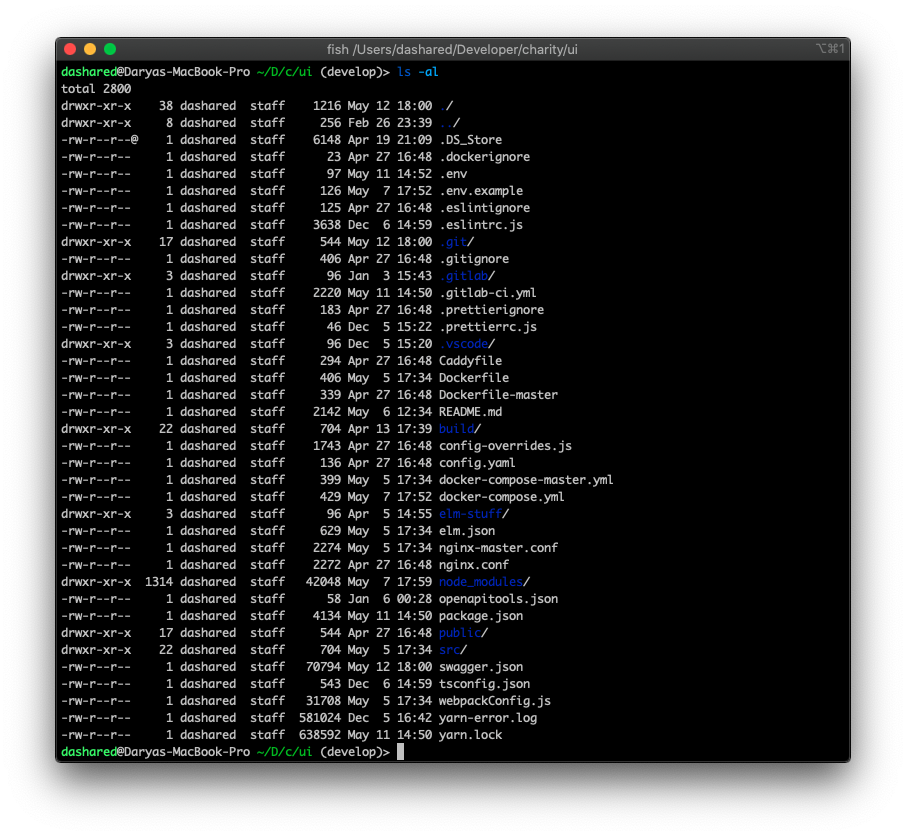
\includegraphics[width = 0.9\linewidth]{img/ro/ls.png}
		\caption{Список файлов корневой папки проекта}
		\label{pic: ls}
	\end{figure}

    Далее с помощью механизмов Docker можно поднять локальную версию Web-приложения следующим образом: в файле \texttt{docker-compose.yml} поменять переменные окружения на \texttt{REACT\_APP\_API\_URL = https://charity.infostrategic.com} и  \texttt{REACT\_APP\_WEBSOCKET = charity.infostrategic.com}. Далее с помощью команды \texttt{docker-compose up -d} развернутое приложение будет доступна по адресу \texttt{localhost:80}.
	
	\subsection{Выполнение программы}
	
	\subsubsection{Стартовая страница}
	
	Для неавторизованных пользователей доступен экран лэндинга приложения (относительный путь \texttt{/}), с описанием модулей CRM-системы для благотворительных фондов <<AIAIN>>. На экране располагается навигационный элемент для перехода на страницу авторизации (кнопка <<Login>>), а также хэдер с возможностью перехода на страницы часто задаваемых вопросов и просмотра информации о фонде (см. скриншоты \ref{pic: landing}).
	
	\begin{figure}[H]
		\centering
		\begin{subfigure}[b]{0.475\linewidth}
			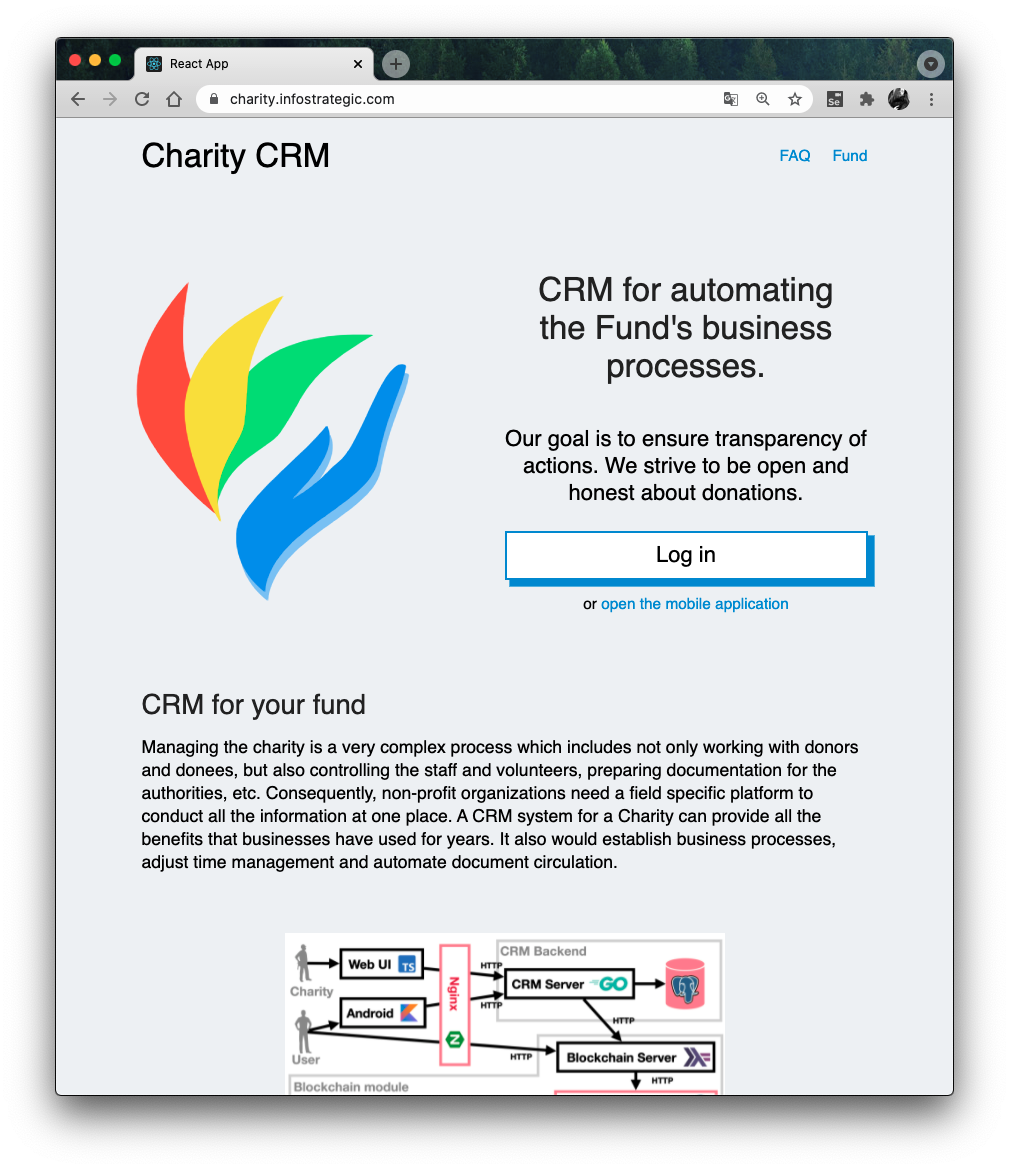
\includegraphics[width=\linewidth]{img/ro/landing.png}
		\end{subfigure}
		\begin{subfigure}[b]{0.475\linewidth}
			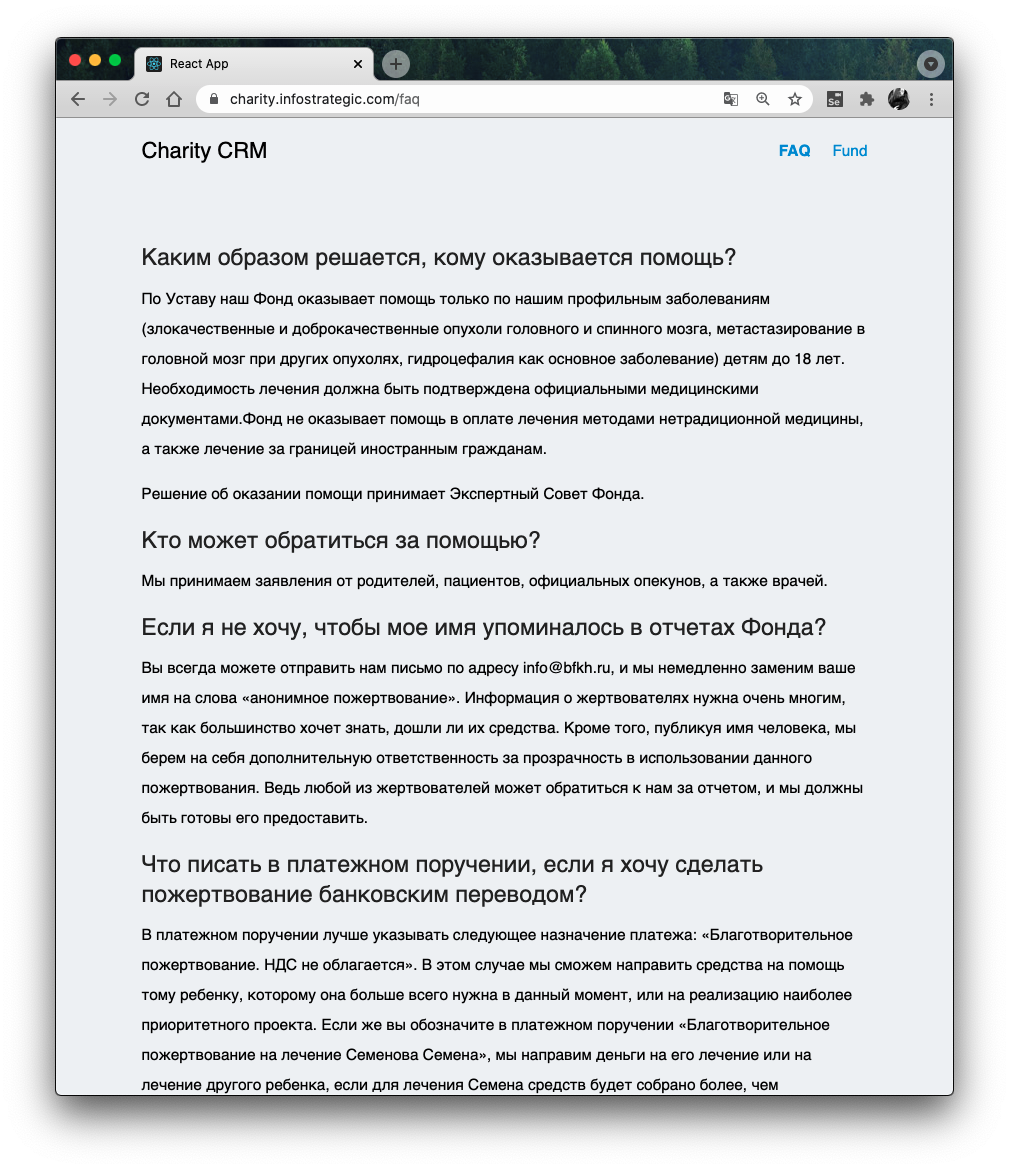
\includegraphics[width=\linewidth]{img/ro/faq_unauthorized.png}
		\end{subfigure}
		\caption{Скриншоты лэндинговой страницы и FAQ для неавторизованных пользователей}
		\label{pic: landing}
	\end{figure}
	
	\subsubsection{Авторизация}
	
	Авторизация в системе происходит со страницы с относительным url \texttt{/login}. На данную страницу можно попасть, нажав на кнопку <<Login>> на лэндинговой странице (см. скриншот \ref{pic: landing}). При авторизации в системе зарегистрированный пользователь должен ввести свой email и пароль в поля в форме (см. скриншот \ref{pic: login}). При неудачной попытке авторизации система продемонстрирует нотификации с текстом, соответствующим причине возникшей ошибки.  
	\begin{figure}[H]
		\centering
		\begin{subfigure}[b]{0.475\linewidth}
			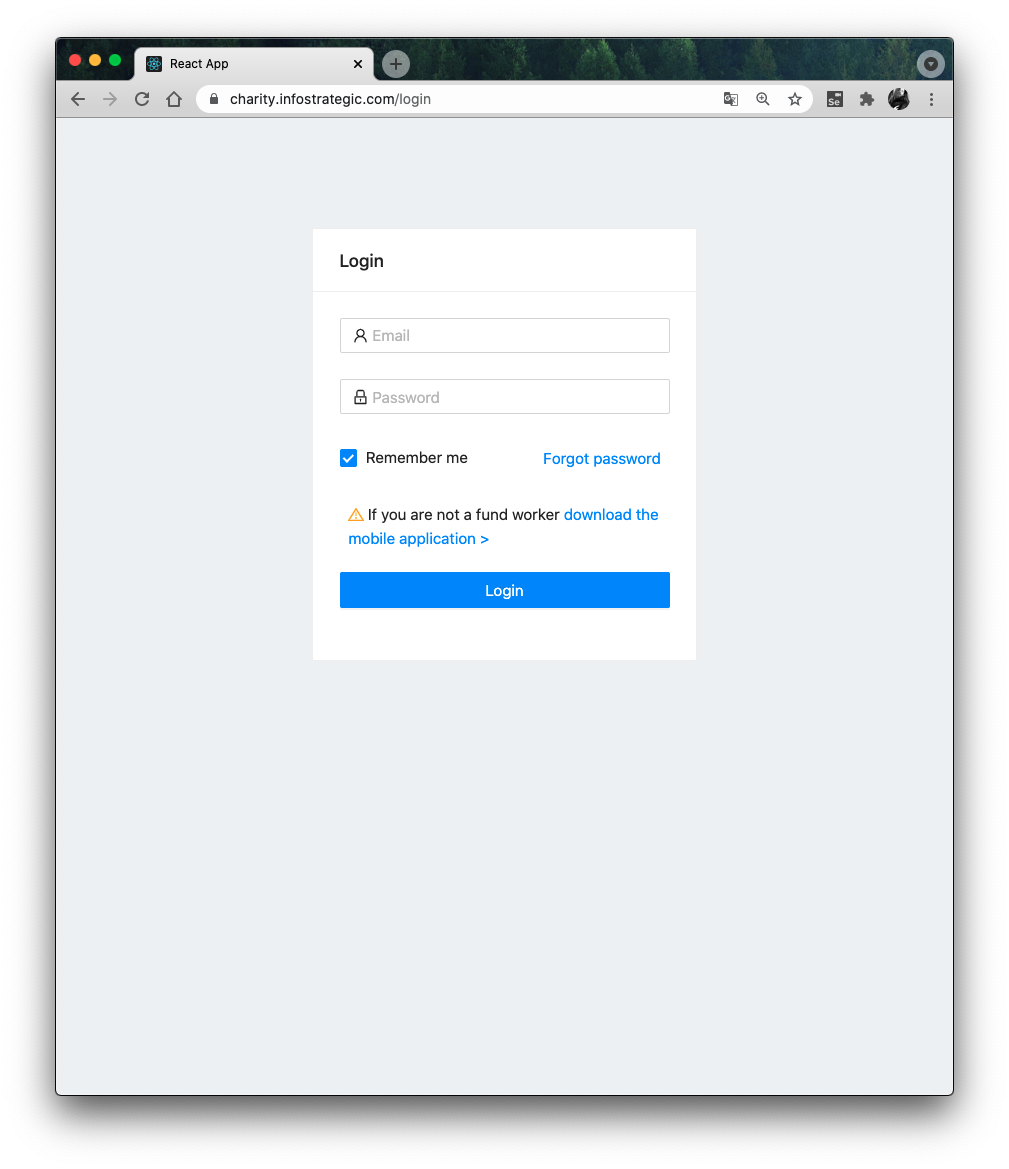
\includegraphics[width=\linewidth]{img/ro/login.png}
		\end{subfigure}
		\begin{subfigure}[b]{0.475\linewidth}
			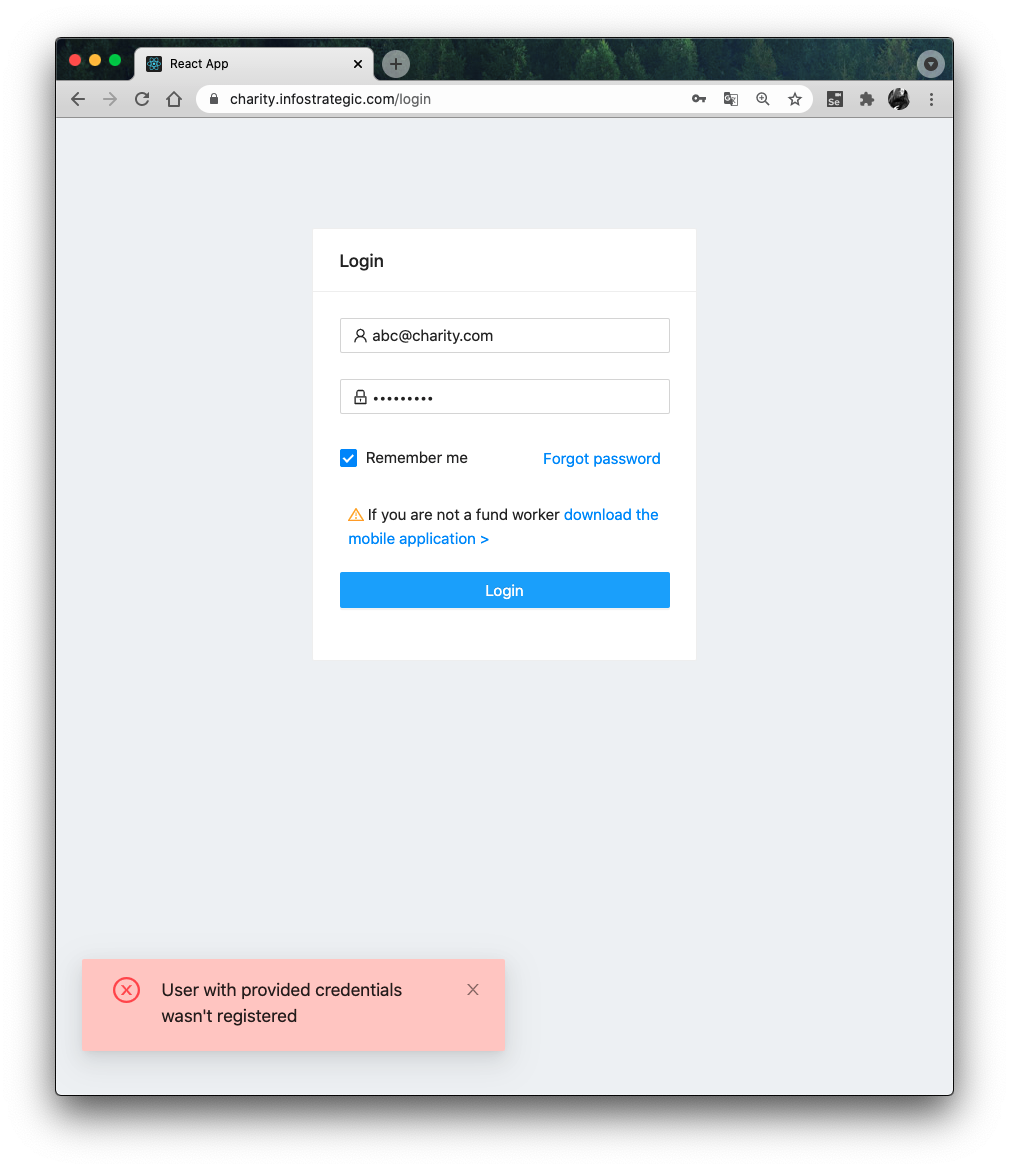
\includegraphics[width=\linewidth]{img/ro/login_error.png}
		\end{subfigure}
		\caption{Скриншоты страницы авторизации}
		\label{pic: login}
	\end{figure}
	
	\subsubsection{Настройки} \label{sec: settings}
	
	Авторизованный пользователь с любой ролью в системе имеет доступ к странице  настроек через url \texttt{/settings} или боковое меню. По кнопке в правом верхнем углу <<Обновить данные>> можно сохранить выбранную информацию о своем профиле, а также изменить язык в системе, выбрав один из двух языков (см. скриншоты \ref{pic: settings}).
	
	\begin{figure}[H]
		\centering
		\begin{subfigure}[b]{0.475\linewidth}
			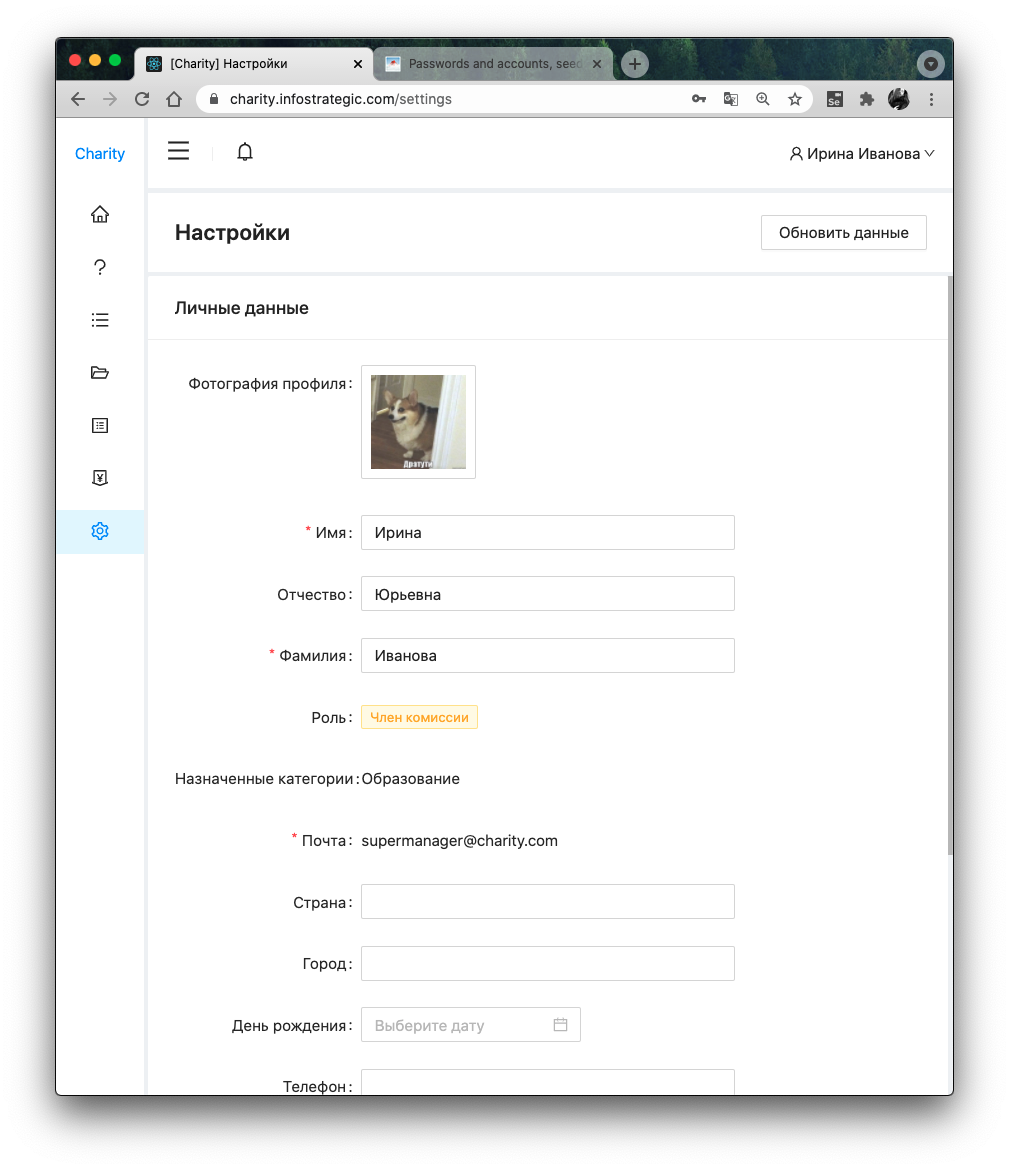
\includegraphics[width=\linewidth]{img/ro/settings.png}
		\end{subfigure}
		\begin{subfigure}[b]{0.475\linewidth}
			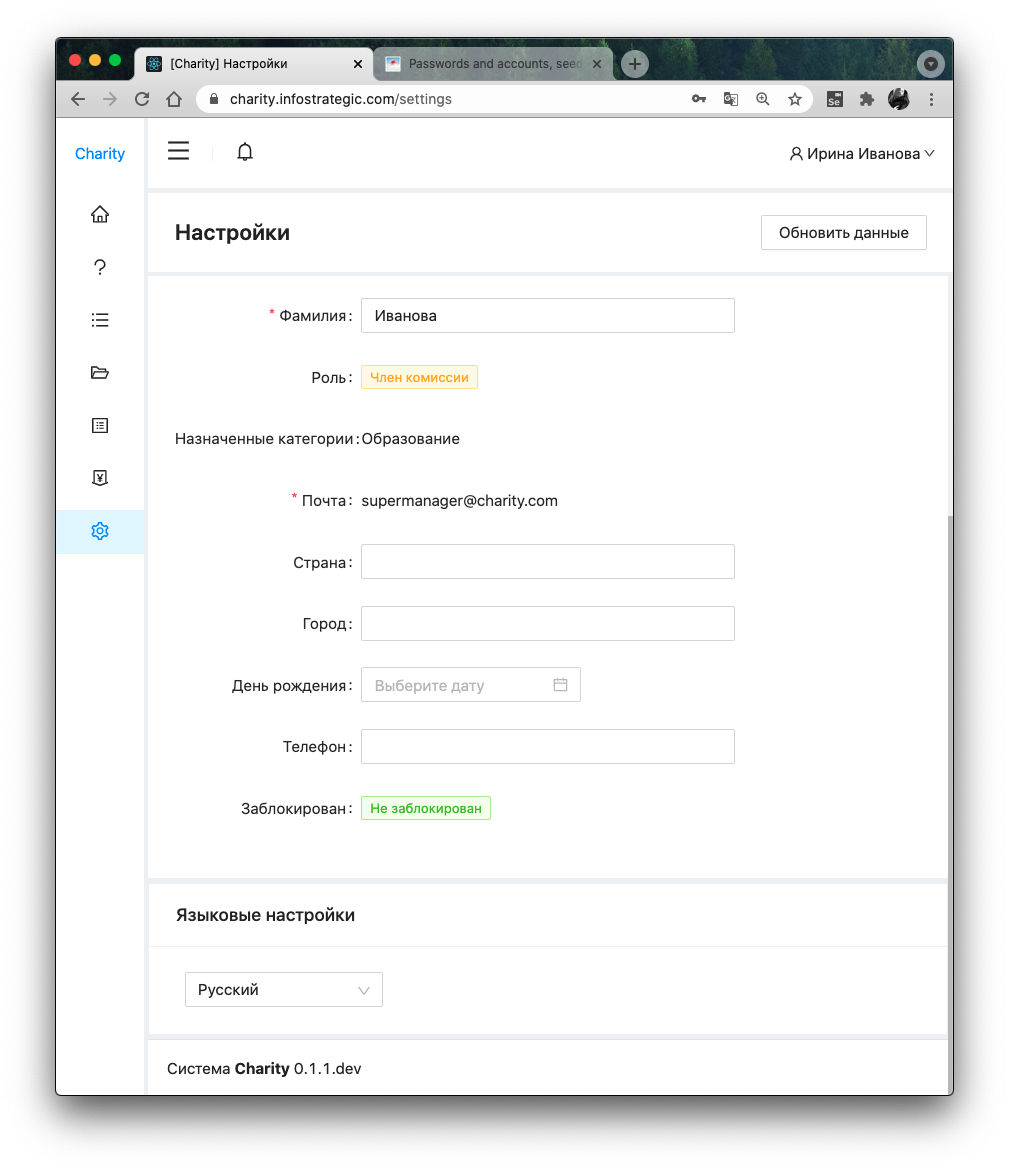
\includegraphics[width=\linewidth]{img/ro/settings_lang.png}
		\end{subfigure}
		\caption{Скриншоты страницы настроек}
		\label{pic: settings}
	\end{figure}
	
	\subsubsection{Уведомления}
	
	Авторизованный пользователь с любой ролью в системе имеет доступ к странице  уведомлений через url \texttt{/notifications} или колокольчик в хэдере. По переключению табов можно увидеть как все пуш-уведомления в системе, так и статусы операций в блокчейн системе (см. скриншоты \ref{pic: notifications}).
	
	\begin{figure}[H]
		\centering
% 		\begin{subfigure}[b]{0.475\linewidth}
% 			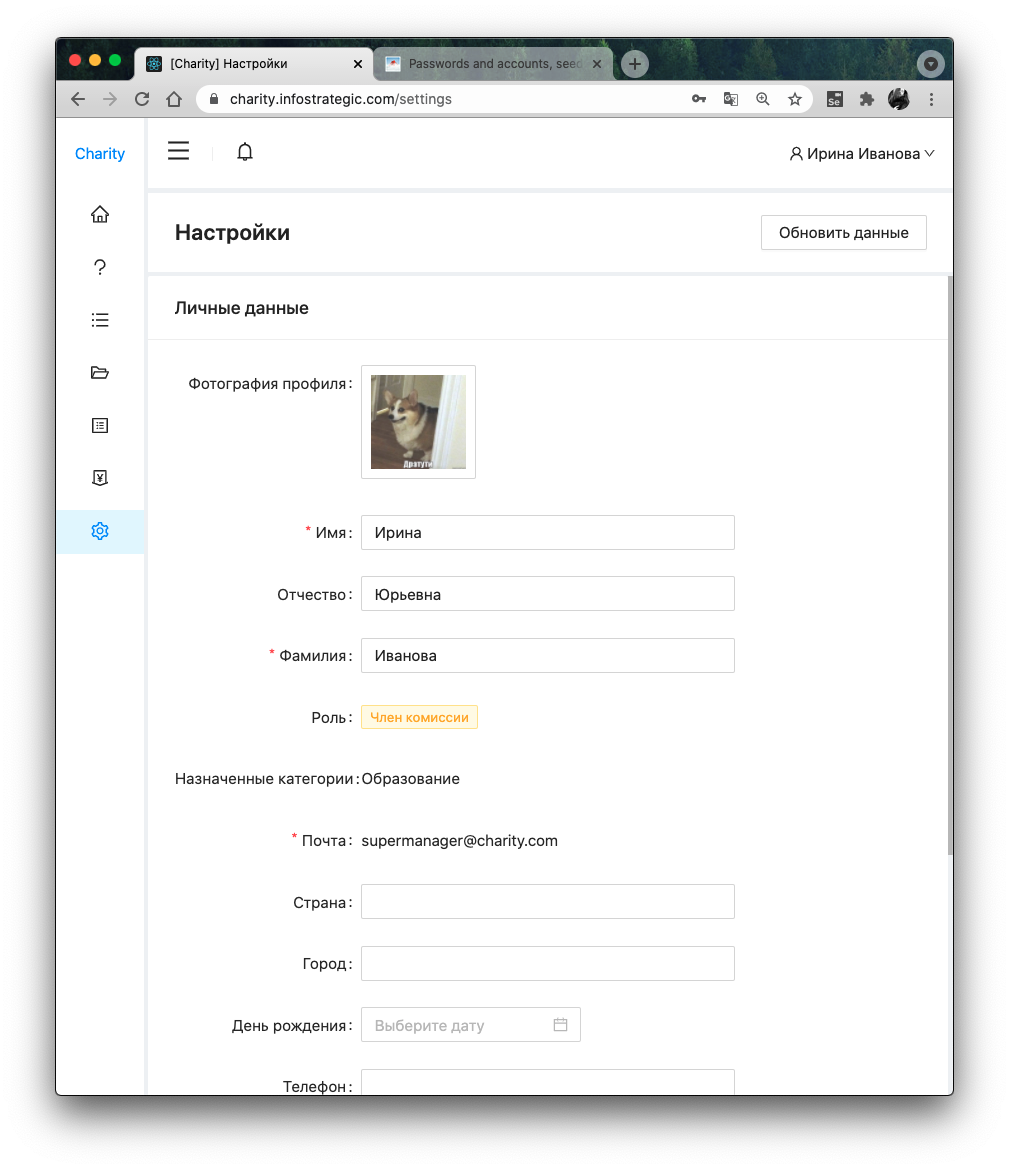
\includegraphics[width=\linewidth]{img/ro/settings.png}
% 		\end{subfigure}
		\begin{subfigure}[b]{0.475\linewidth}
			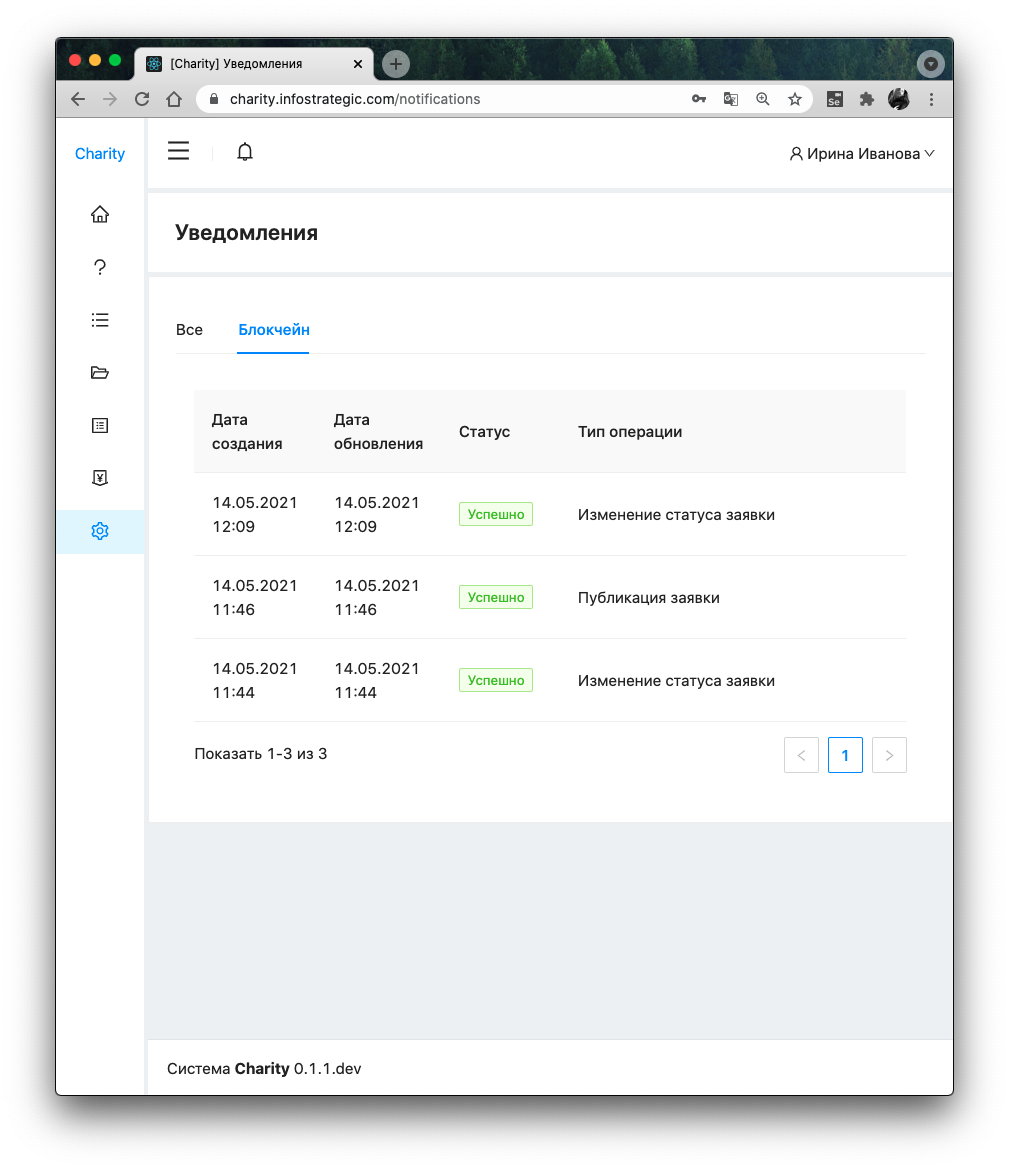
\includegraphics[width=\linewidth]{img/ro/notifications_blockckain.png}
		\end{subfigure}
		\caption{Скриншоты страницы уведомлений}
		\label{pic: notifications}
	\end{figure}
	
	\subsubsection{Функционал администратора}
	
	При авторизации под аккаунтом пользователя с ролью <<Администратор>>, пользователь попадает на страницу с относительным url \texttt{/users} со списком пользователей системы (см. скриншоты \ref{pic: users}). Есть возможность отсортировать, а также отфильтровать пользователей по роли.
	
	\begin{figure}[H]
		\centering
		\begin{subfigure}[b]{0.475\linewidth}
			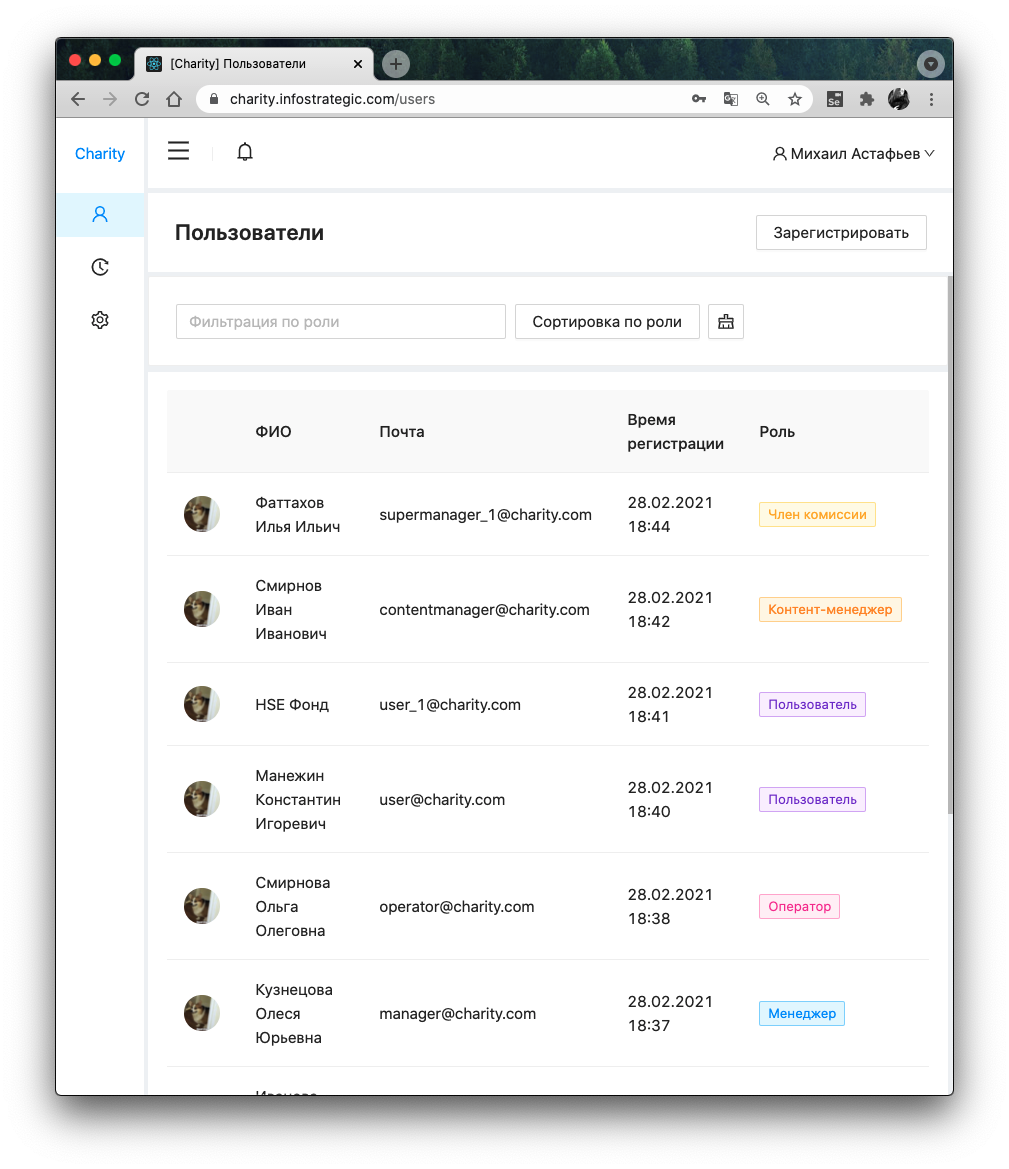
\includegraphics[width=\linewidth]{img/ro/users.png}
		\end{subfigure}
		\begin{subfigure}[b]{0.475\linewidth}
			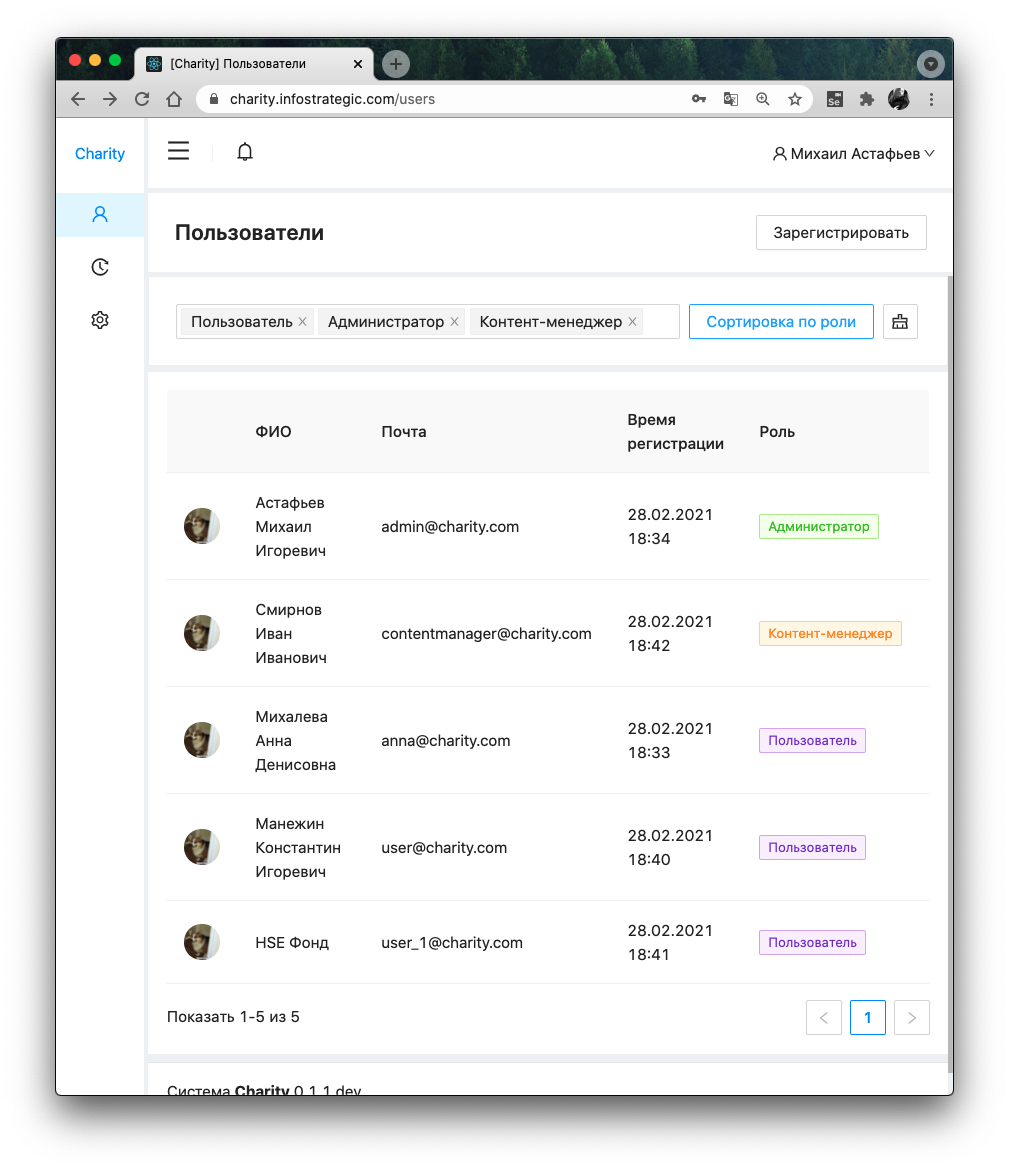
\includegraphics[width=\linewidth]{img/ro/users_filtered.png}
		\end{subfigure}
		\caption{Скриншоты страницы списка пользователей}
		\label{pic: users}
	\end{figure}
	
	В верхнем правом углу расположена кнопка <<Зарегистрировать>>, нажав на которую администратор может зарегистрировать пользователя в системе, указав его ФИО, почту, желаемую роль и назначенные категории (только для пользователей с ролью <<Член комисии>>). Страница располагается по относительному адресу \texttt{/users/create}. Кнопка <<Очистить>> позволяет очистить ранее заполненные поля формы. При успешной регистрации по кнопке <<Зарегистрировать>> пользователь попадает на страницу \texttt{/users} со списком пользователей, в котором можно увидеть только что зарегистрированного пользователя (см. скриншоты \ref{pic: users}).
	
	\begin{figure}[H]
		\centering
		\begin{subfigure}[b]{0.475\linewidth}
			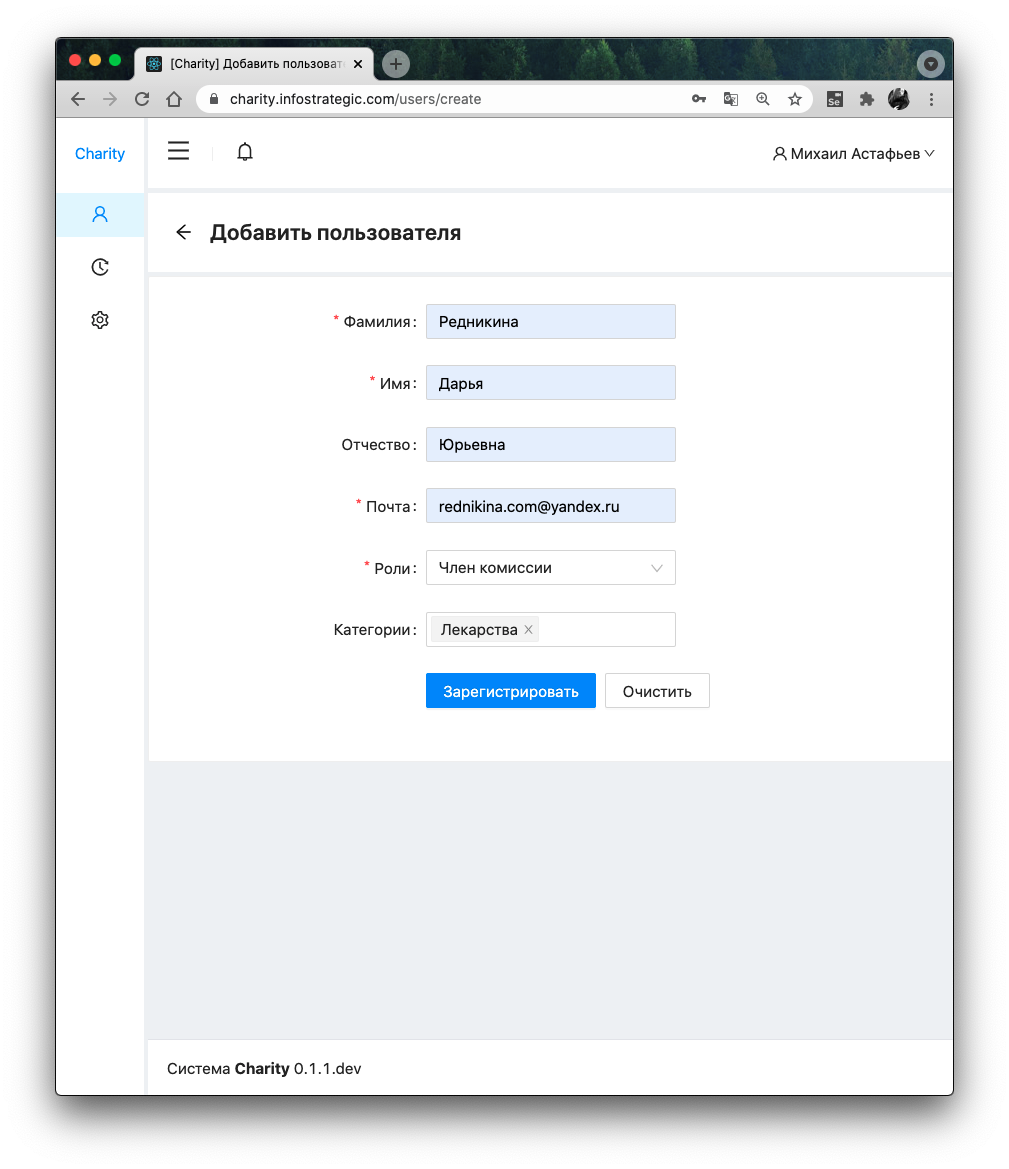
\includegraphics[width=\linewidth]{img/ro/reg_filled.png}
		\end{subfigure}
		\begin{subfigure}[b]{0.475\linewidth}
			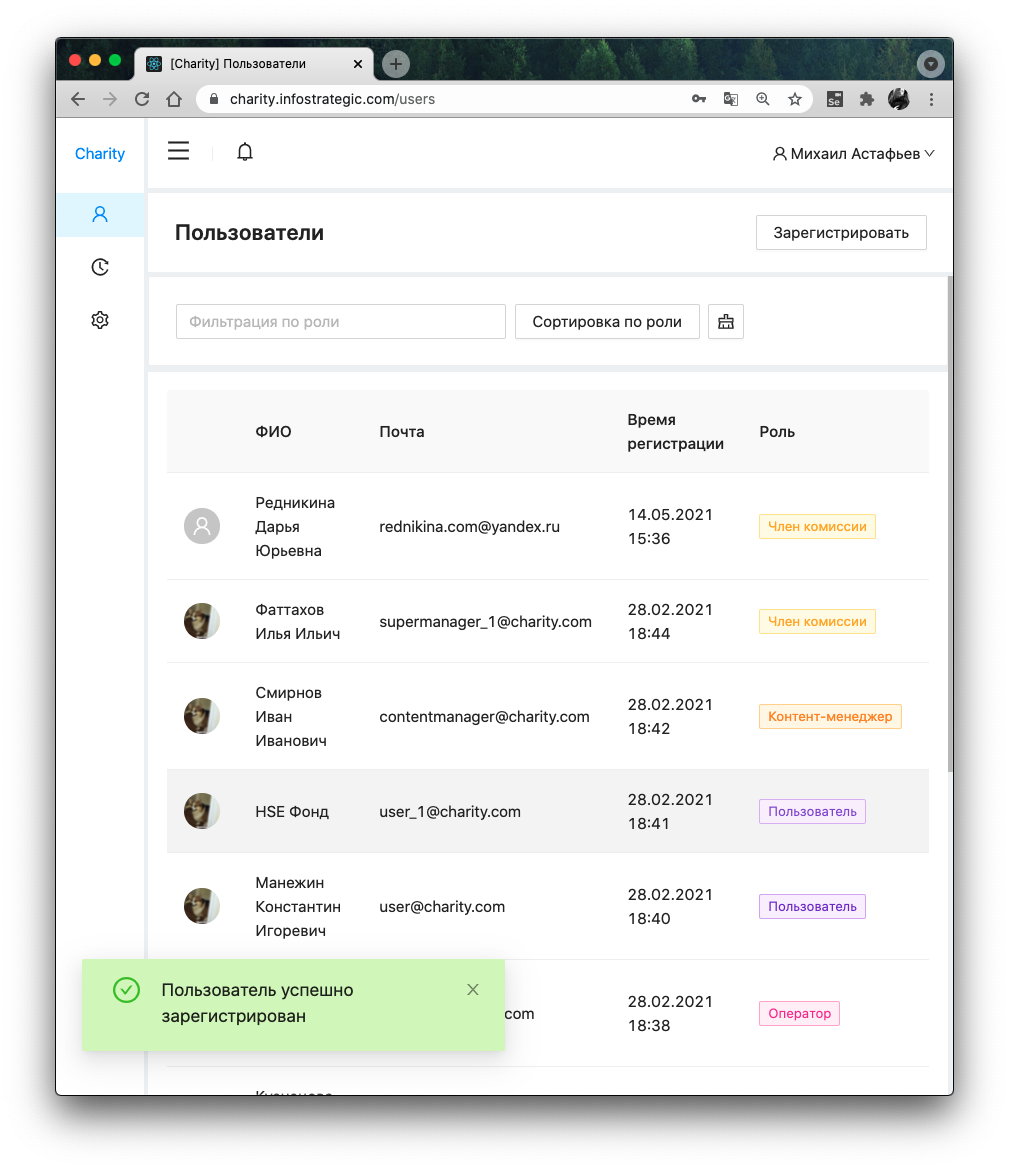
\includegraphics[width=\linewidth]{img/ro/reg_success.png}
		\end{subfigure}
		\caption{Скриншоты страницы регистрации пользователей}
		\label{pic: users}
	\end{figure}
	
	Перейдя на страницу пользователя из списка пользователей по клику на соответствующий ряд, администратор может как посмотреть полную информацию о пользователе (см. скриншот \ref{pic: user}), так и отредактировать ее (только те поля, которые доступны для редактирования) по кнопке в правом верхнем углу <<Обновить данные>>. 
	
	\begin{figure}[H]
		\centering
		\begin{subfigure}[b]{0.475\linewidth}
			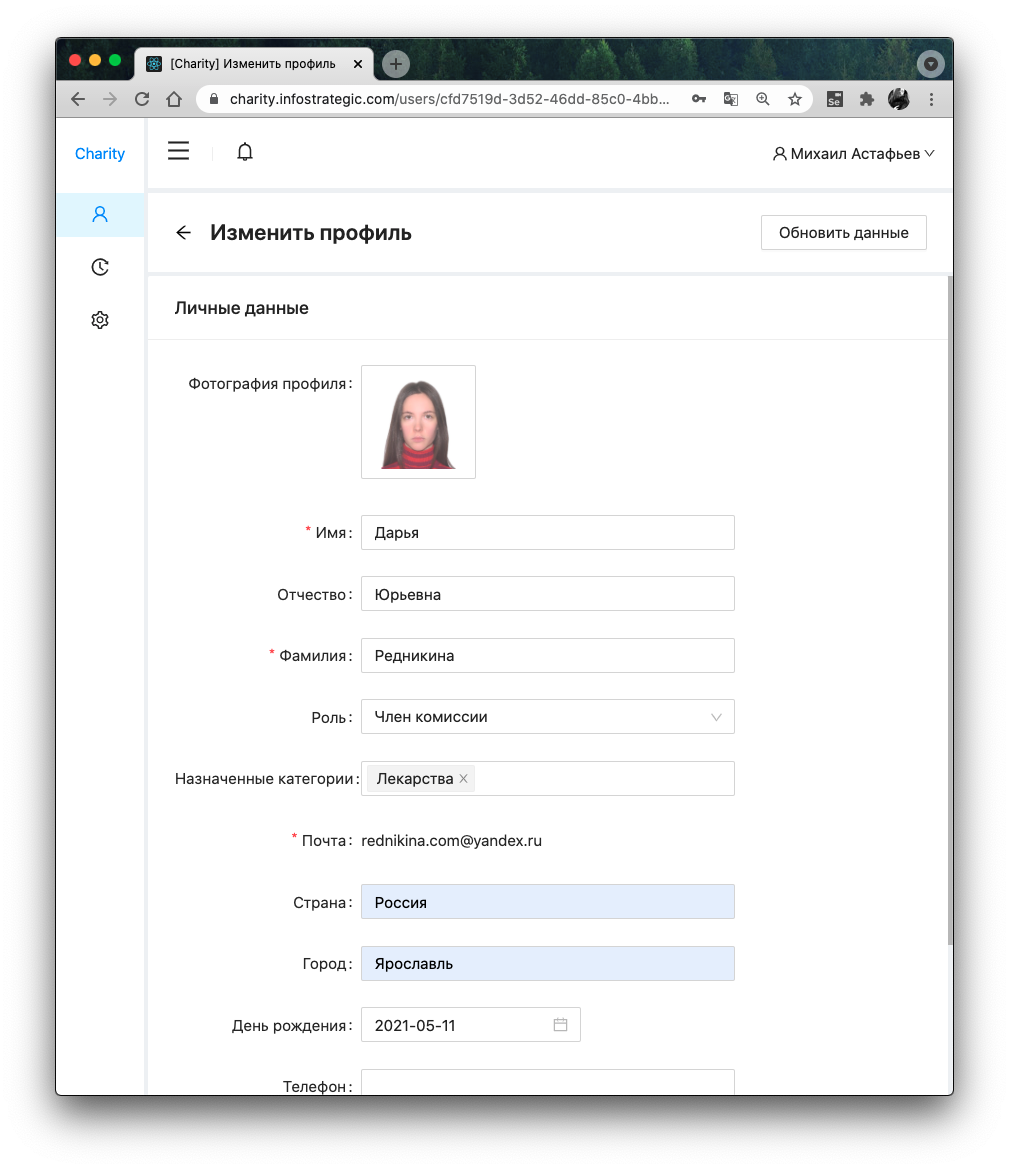
\includegraphics[width=\linewidth]{img/ro/user_upd.png}
		\end{subfigure}
		\begin{subfigure}[b]{0.475\linewidth}
			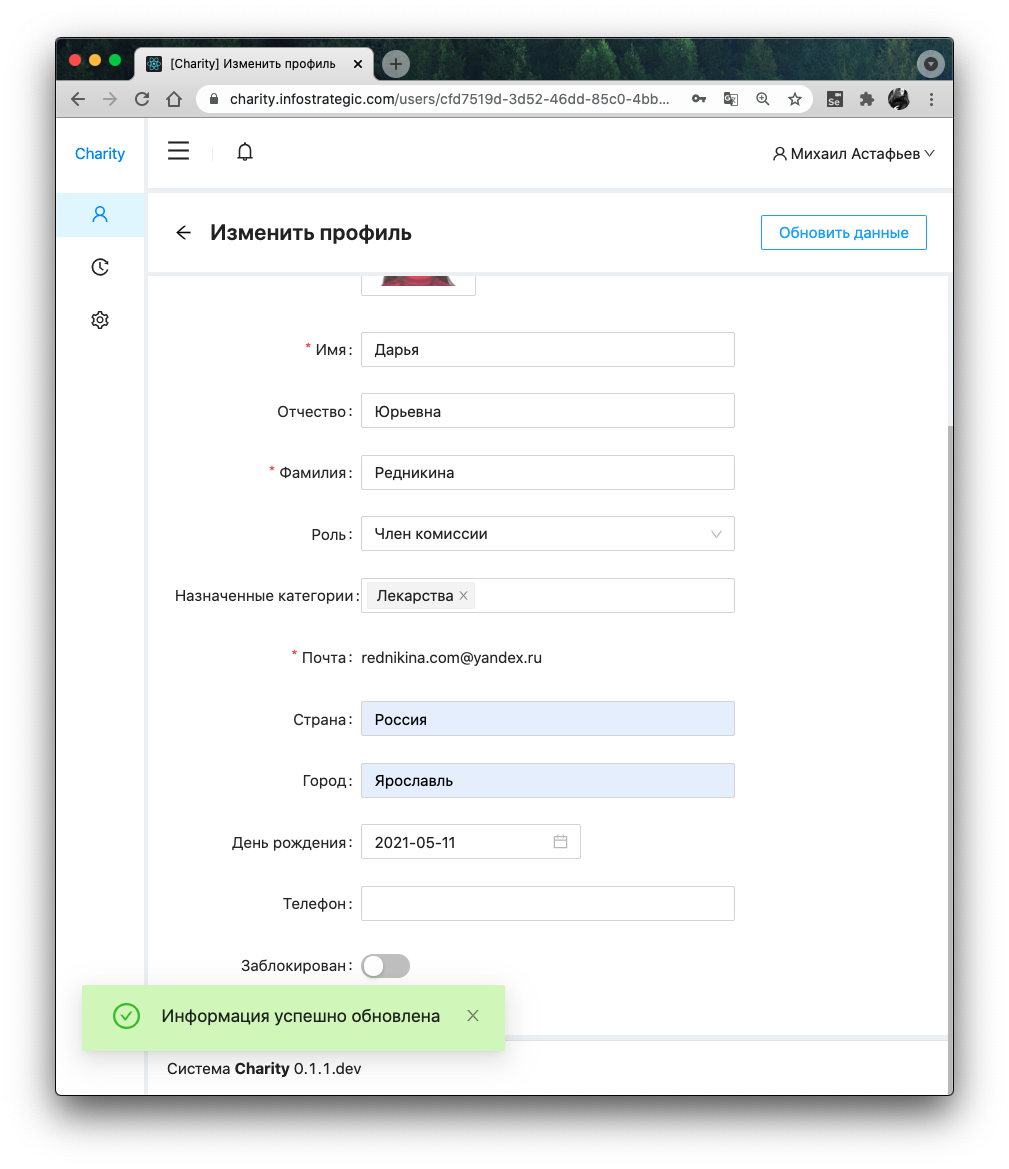
\includegraphics[width=\linewidth]{img/ro/user_upd_success.png}
		\end{subfigure}
		\caption{Скриншоты страницы редактирования пользователя}
		\label{pic: user}
	\end{figure}
	
	Также администратор через боковую панель или по относительному пути \texttt{/logs} может перейти в список логов (см. скриншот \ref{pic: logs}). Можно также раскрыть каждую ячейку в таблице для получения более полной информации о залогированном событии.
	
	\begin{figure}[H]
		\centering
		\begin{subfigure}[b]{0.475\linewidth}
			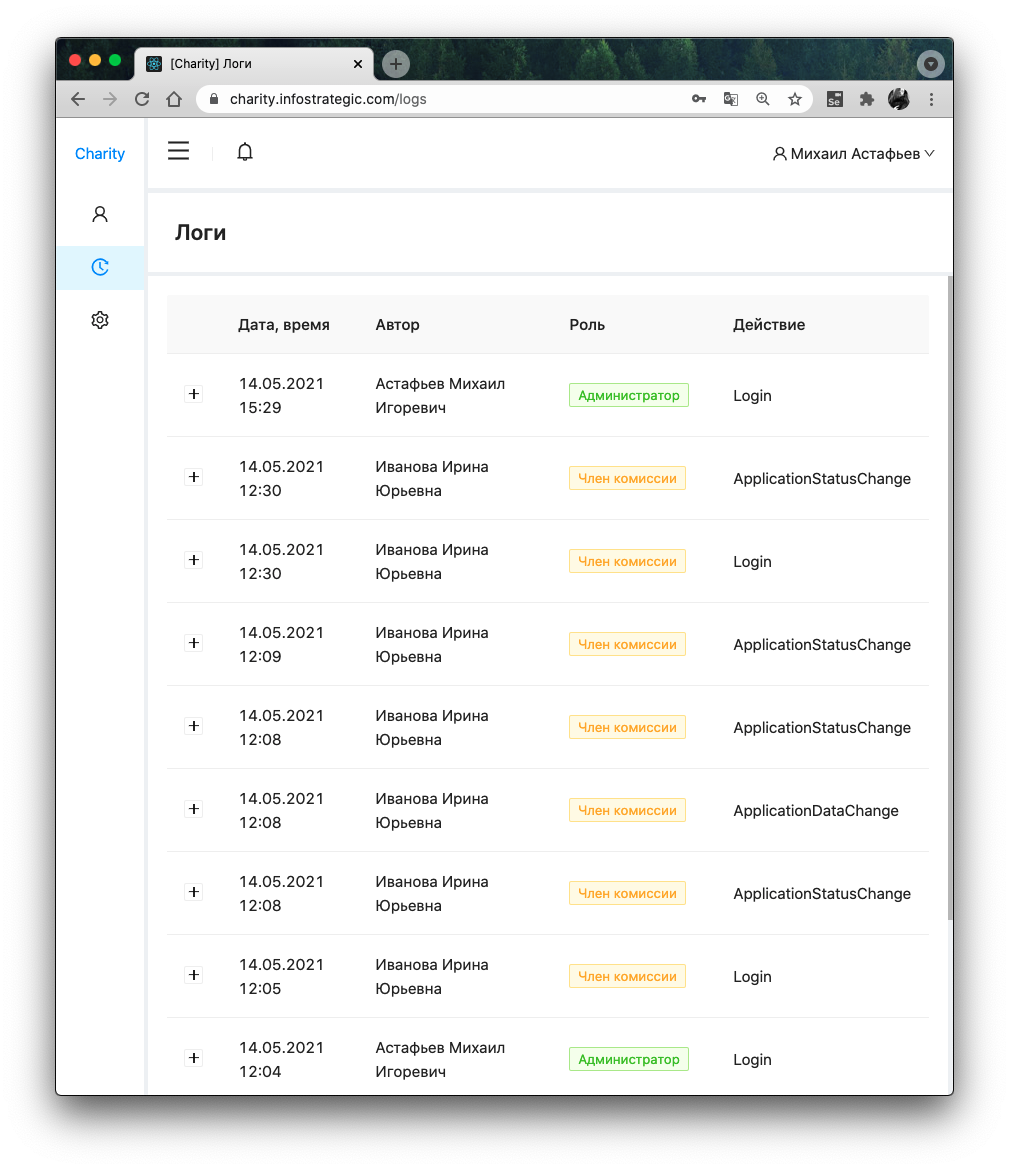
\includegraphics[width=\linewidth]{img/ro/logs.png}
		\end{subfigure}
		\begin{subfigure}[b]{0.475\linewidth}
			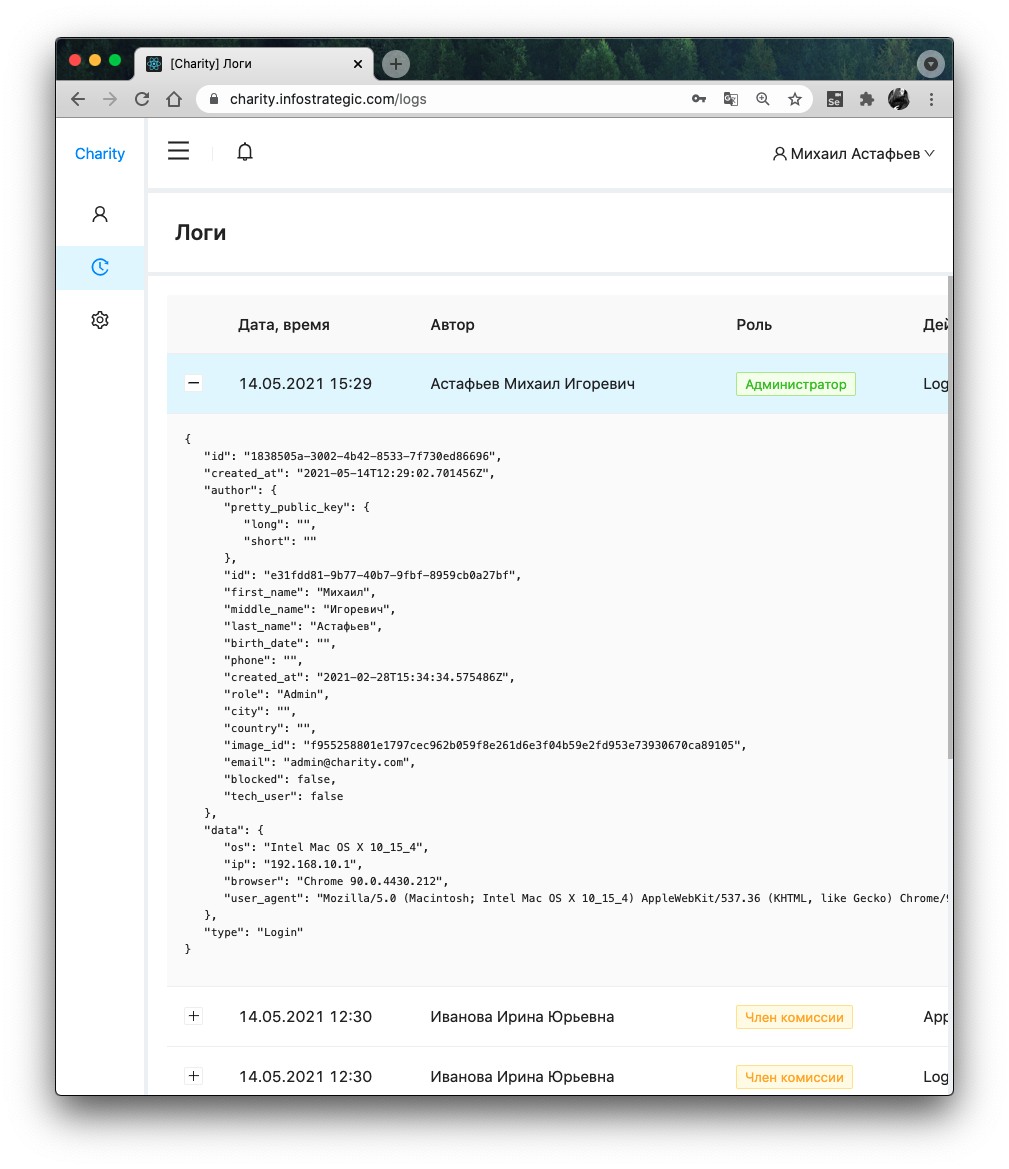
\includegraphics[width=\linewidth]{img/ro/logs_open.png}
		\end{subfigure}
		\caption{Скриншоты страницы логов}
		\label{pic: logs}
	\end{figure}
	
	\subsubsection{Функционал менеджера контента}
	
	Менеджер-контента может перейти на страницу с информацией о фонда через относительный url \texttt{/fund/description} или через соответствующее боковое навигационное меню <<Описание>>. На странице с информацией о фонде можно как просмотреть уже заполненные данные (см. скриншот \ref{pic: fund_description}), так и отредактировать информацию, нажав на кнопку <<Сохранить>> в правом верхнем углу.
	
	\begin{figure}[H]
		\centering
		\begin{subfigure}[b]{0.475\linewidth}
			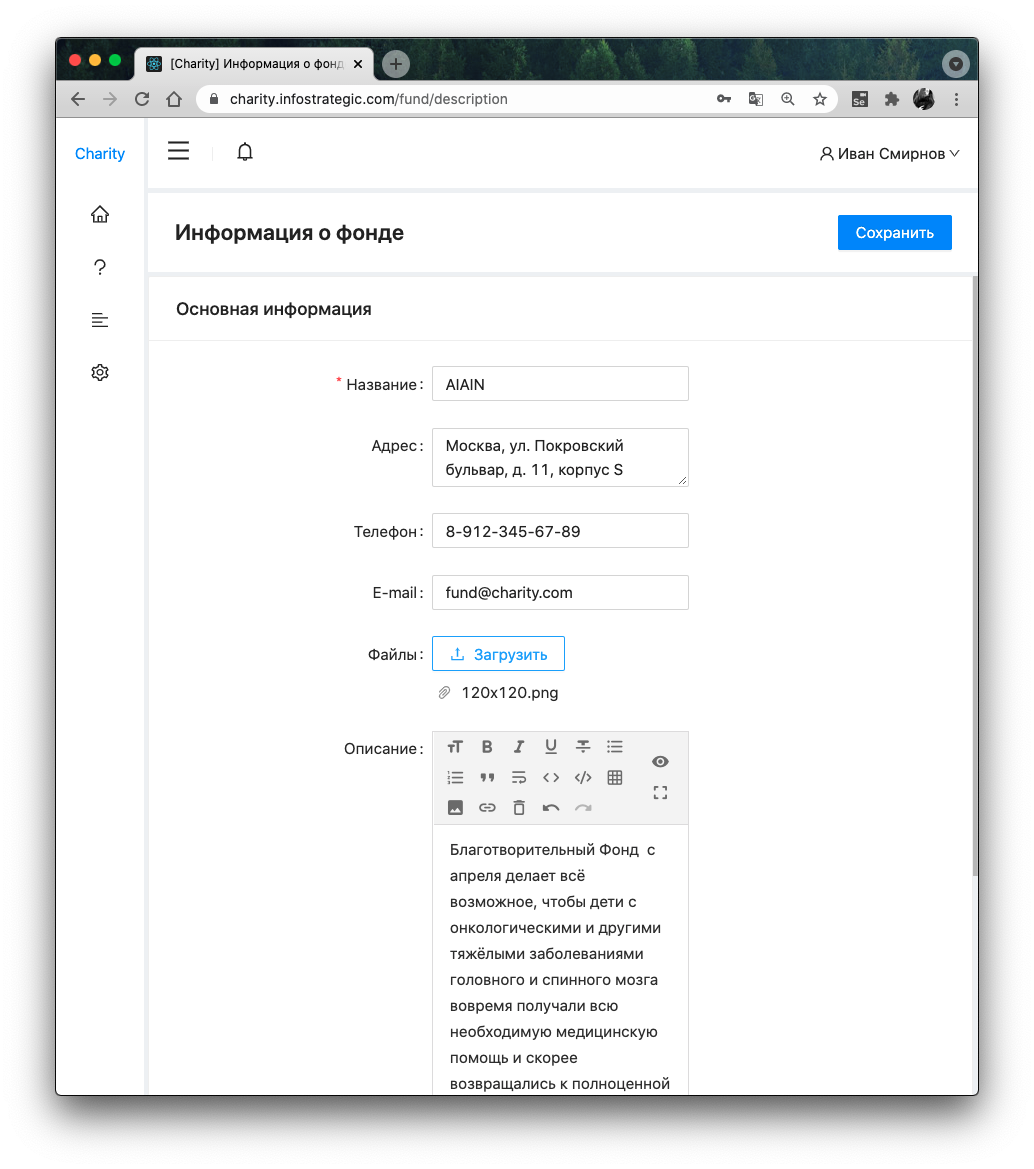
\includegraphics[width=\linewidth]{img/ro/fund_description.png}
		\end{subfigure}
		\caption{Скриншот описания фонда}
		\label{pic: fund_description}
	\end{figure}
	
	Также контент-менеджер может перейти на страницу со списком новостей фонда через боковую панель или через относительный url \texttt{/news}. По кнопке в правом верхнем углу менеджер может перейти на экран публикации новости (или через относительный путь \texttt{/news/create}), после, заполнив необходимые поля (см. скриншот \ref{pic: news}) по кнопке в правом верхнем углу <<Опубликовать>> новость будет размещена в списке новостей. Также в списке новостей в ряду с информацией о каждой новости есть кнопки для удаления и редактирования.
	
	\begin{figure}[H]
		\centering
		\begin{subfigure}[b]{0.475\linewidth}
			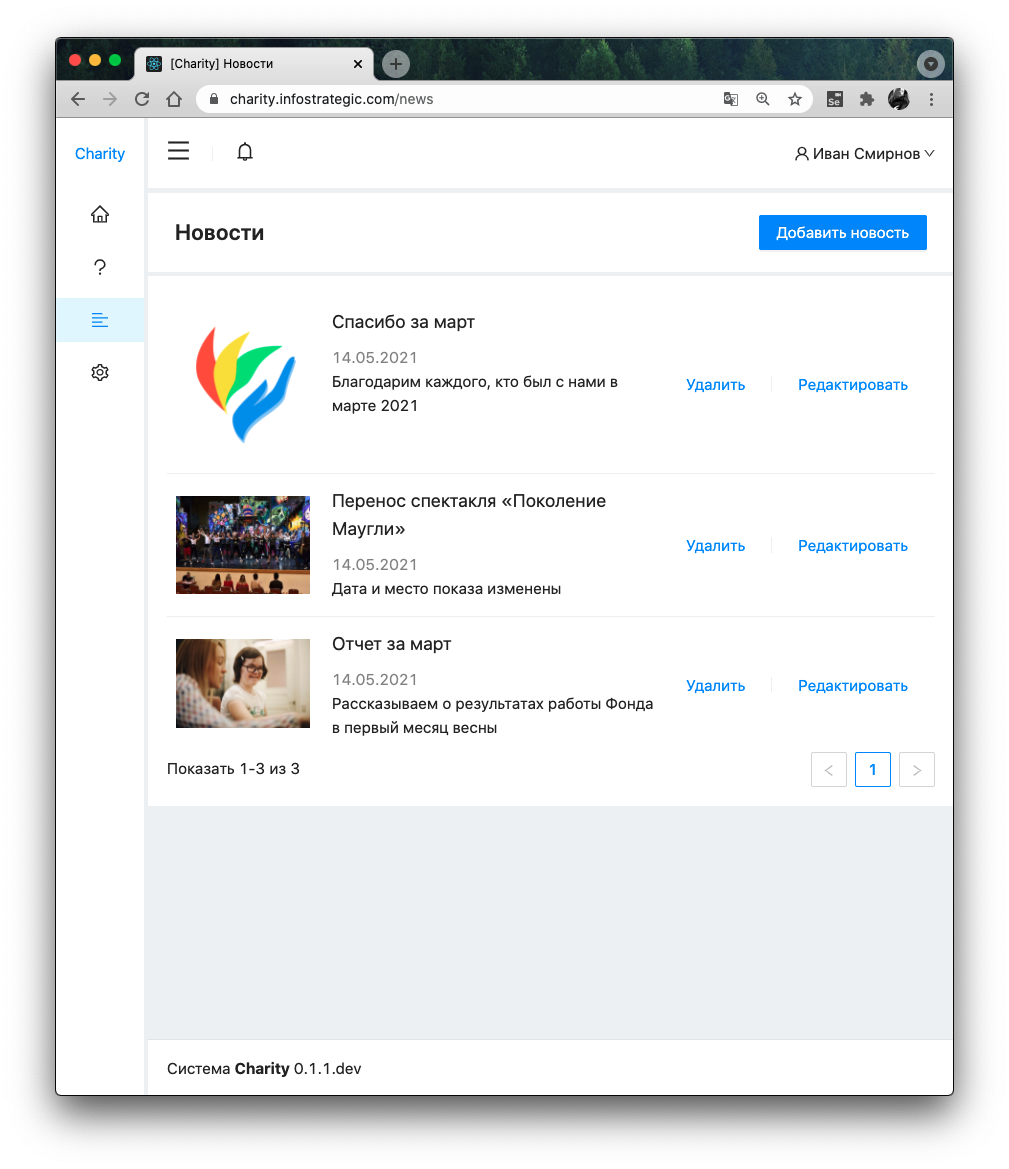
\includegraphics[width=\linewidth]{img/ro/news.png}
		\end{subfigure}
		\begin{subfigure}[b]{0.475\linewidth}
			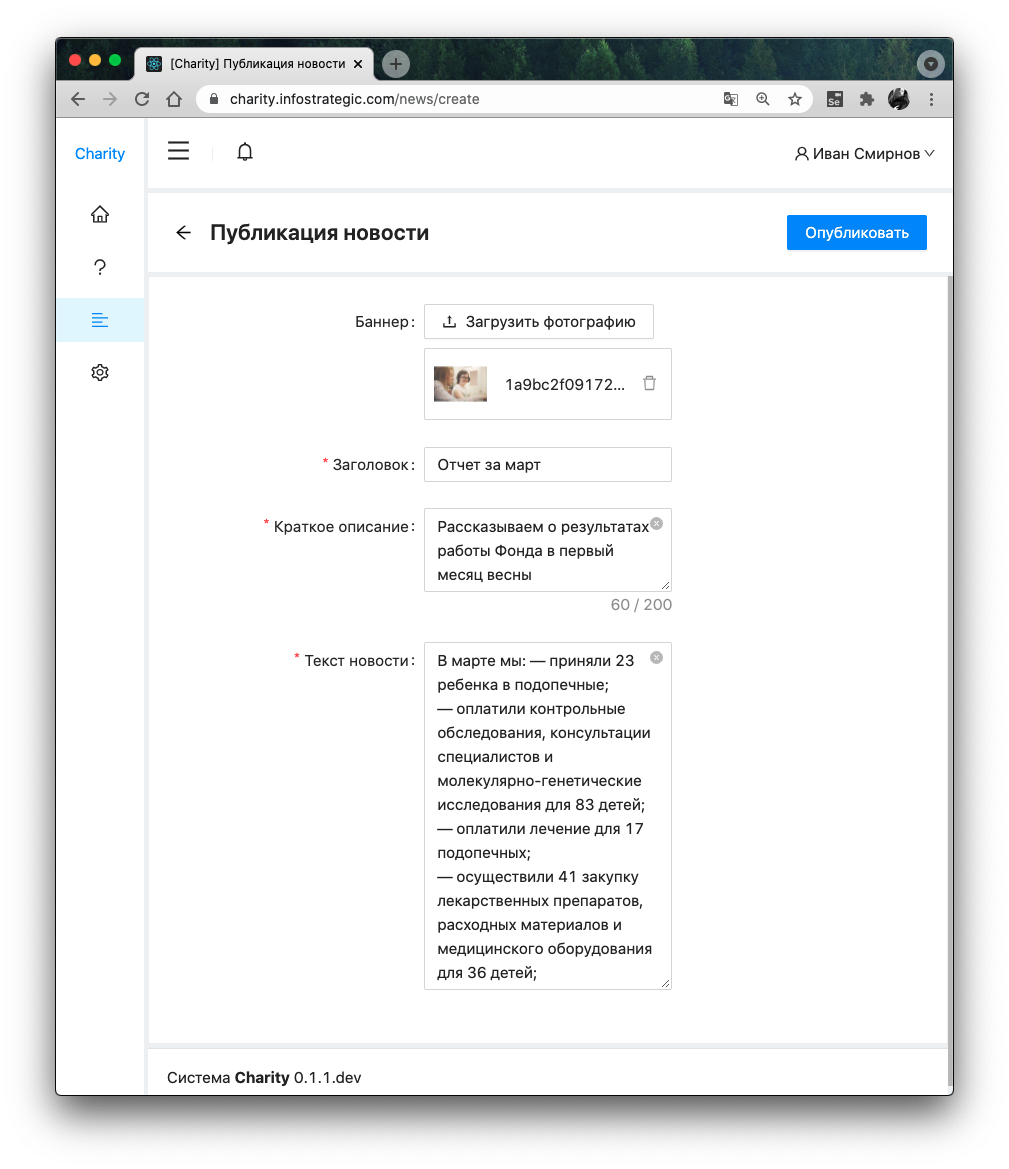
\includegraphics[width=\linewidth]{img/ro/news_publish.png}
		\end{subfigure}
		\caption{Скриншоты публикации и списка новостей}
		\label{pic: news}
	\end{figure}
	
	Контент-менеджер может перейти на страницу со списком новостей фонда через боковую панель или через относительный url \texttt{/faq}. В редакторе в формате markdown~\cite{md} пользователь может просмотреть или отредактировать текст, сохранив изменения по кнопке <<Сохранить>>, расположенной в верхнем правом углу (см. скриншоты \ref{pic: faq}).
	
	\begin{figure}[H]
		\centering
		\begin{subfigure}[b]{0.475\linewidth}
			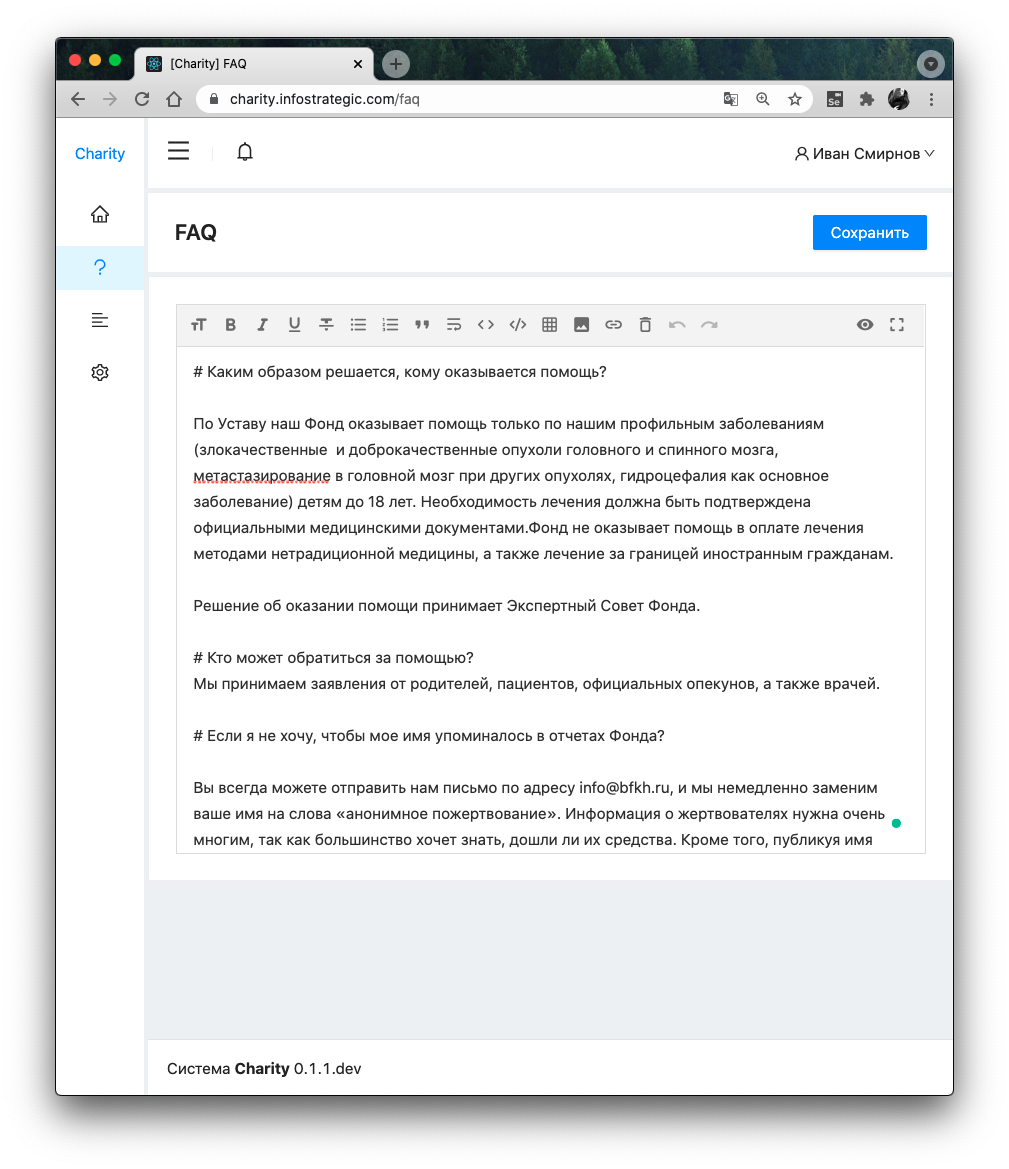
\includegraphics[width=\linewidth]{img/ro/faq.png}
		\end{subfigure}
		\begin{subfigure}[b]{0.475\linewidth}
			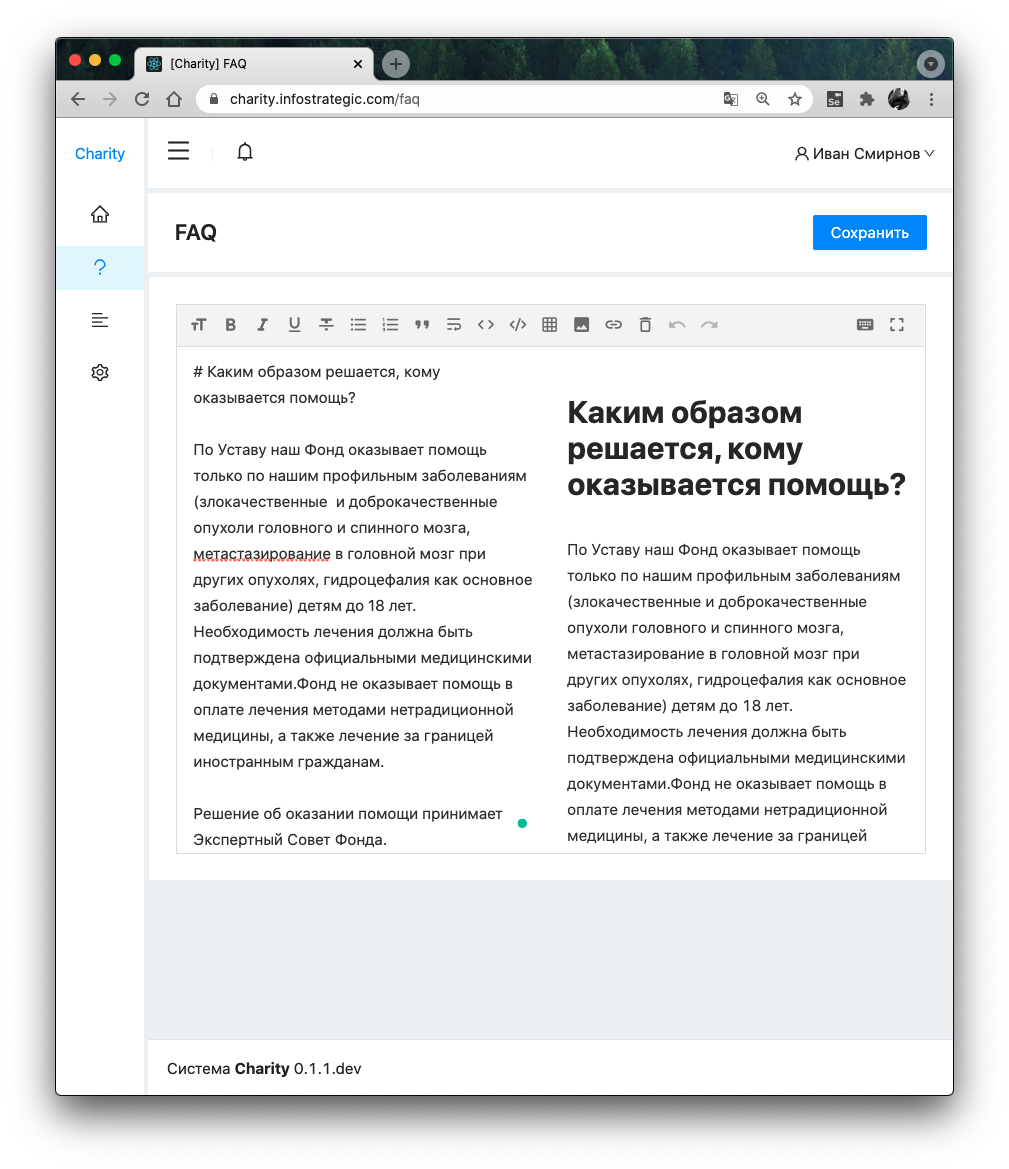
\includegraphics[width=\linewidth]{img/ro/faq_1.png}
		\end{subfigure}
		\caption{Скриншоты редактировании часто задаваемых вопросов}
		\label{pic: faq}
	\end{figure}
	
	\subsubsection{Функционал менеджера} \label{sec: man}
	
	При авторизации в приложении пользователи с ролью <<Менеджер>> попадают на страницу со списком заявок с относительным адресом \texttt{/applications}. У менеджеров есть возможность пофильтровать заявки по статусам и по признаку назначена ли эта заявка на менеджера (см. скриншоты \ref{pic: applications_m}). 
	
	\begin{figure}[H]
		\centering
		\begin{subfigure}[b]{0.475\linewidth}
			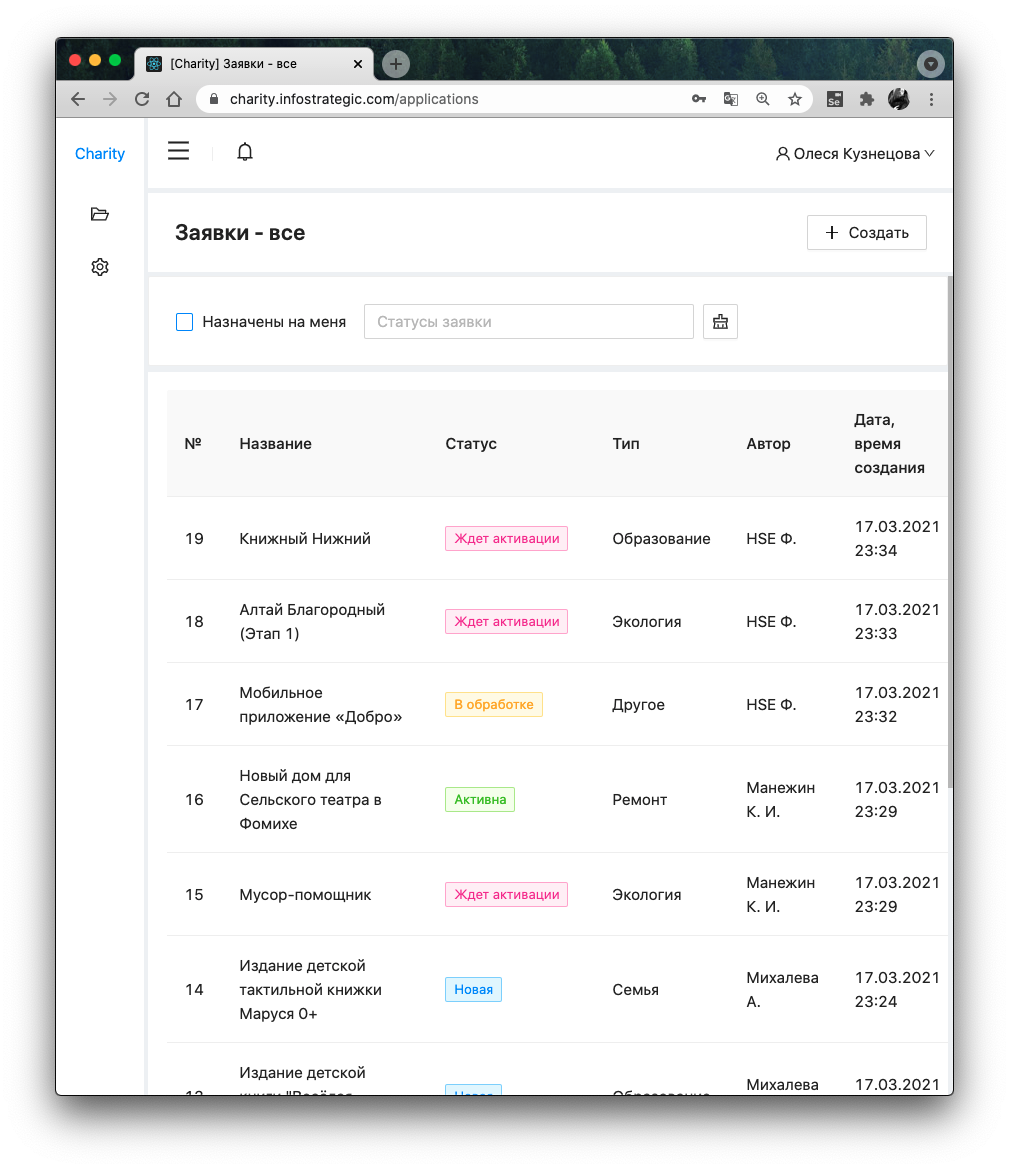
\includegraphics[width=\linewidth]{img/ro/applications_manager.png}
		\end{subfigure}
		\begin{subfigure}[b]{0.475\linewidth}
			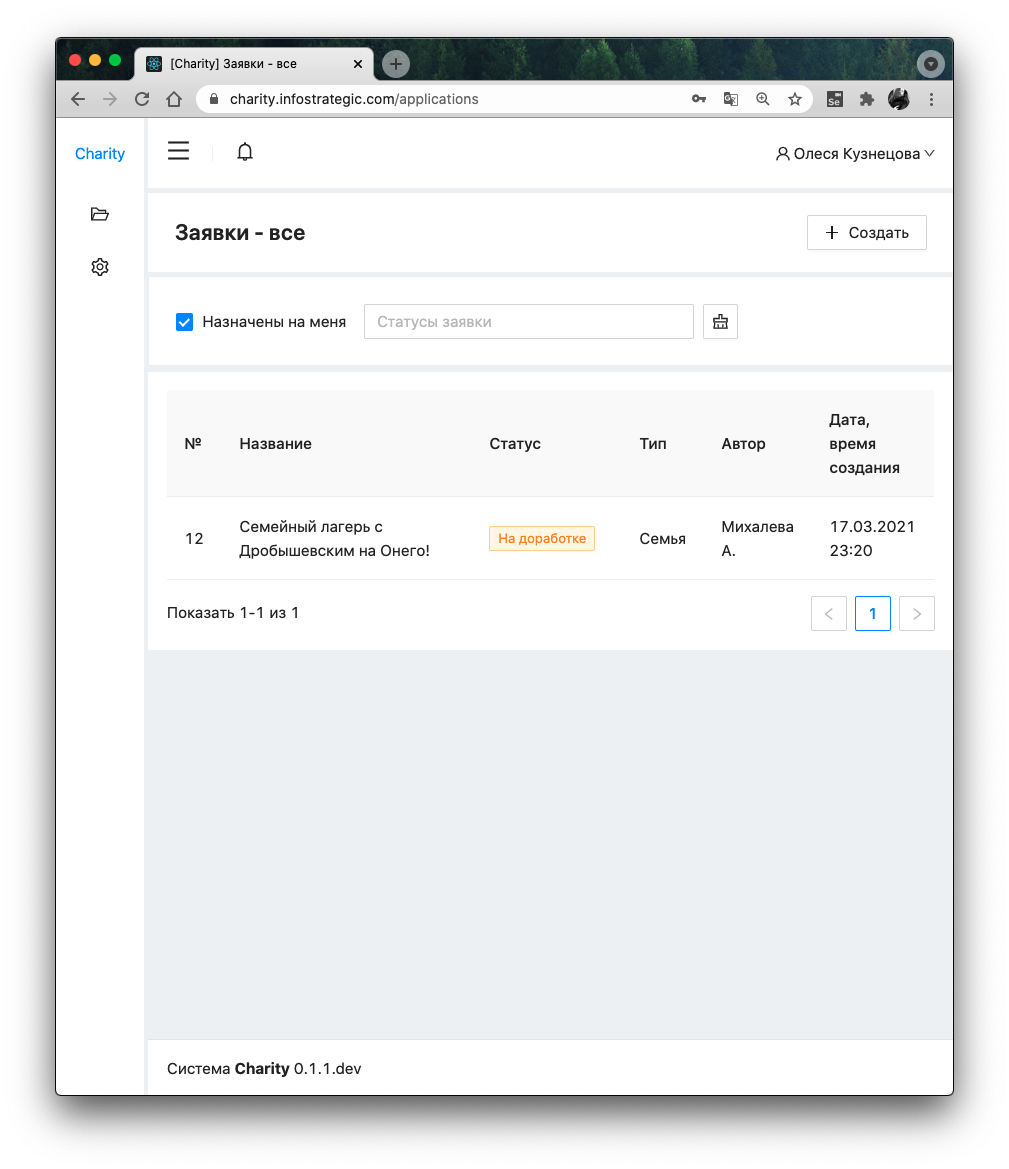
\includegraphics[width=\linewidth]{img/ro/applications_m_filter.png}
		\end{subfigure}
		\caption{Скриншоты страницы заявок, менеджер}
		\label{pic: applications_m}
	\end{figure}
	
	По нажатию на одну из заявок в списке менеджер попадает на страницу заявки (см. скриншот \ref{pic: application_tabs}). По кнопке в правом верхнем углу <<Действия с заявкой>> менеджер может инициировать открытие бокового меню, в котором есть возможность выбрать один из статусов для перевода заявки. Также менеджер может добавить комментарий к изменению статуса заявки, который потом будет отображаться в общем списке комментариев к заявке (см. скриншот \ref{pic: application_tabs}).
	
	
	\begin{figure}[H]
		\centering
		\begin{subfigure}[b]{0.475\linewidth}
			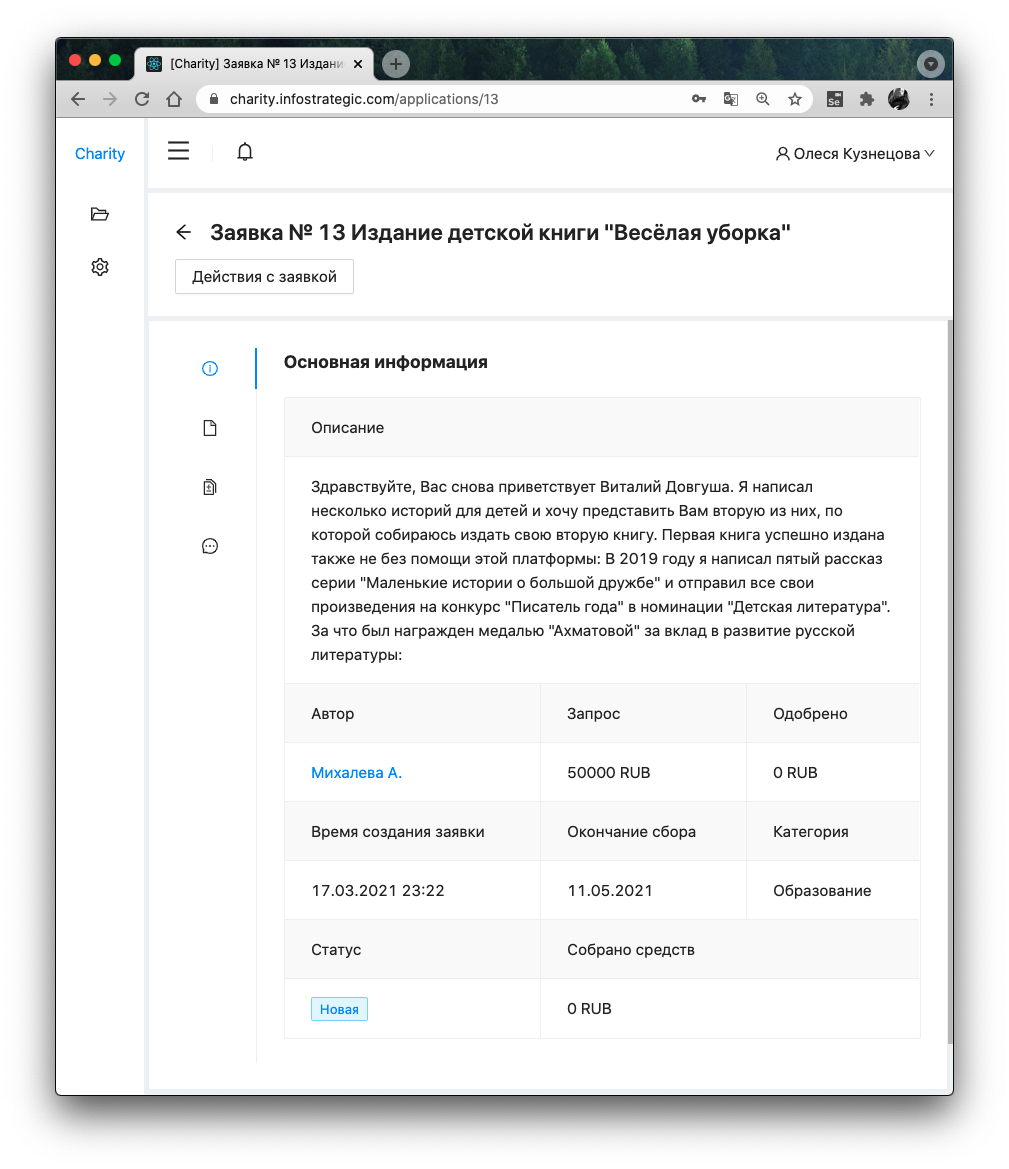
\includegraphics[width=\linewidth]{img/ro/application.png}
		\end{subfigure}
		\begin{subfigure}[b]{0.475\linewidth}
			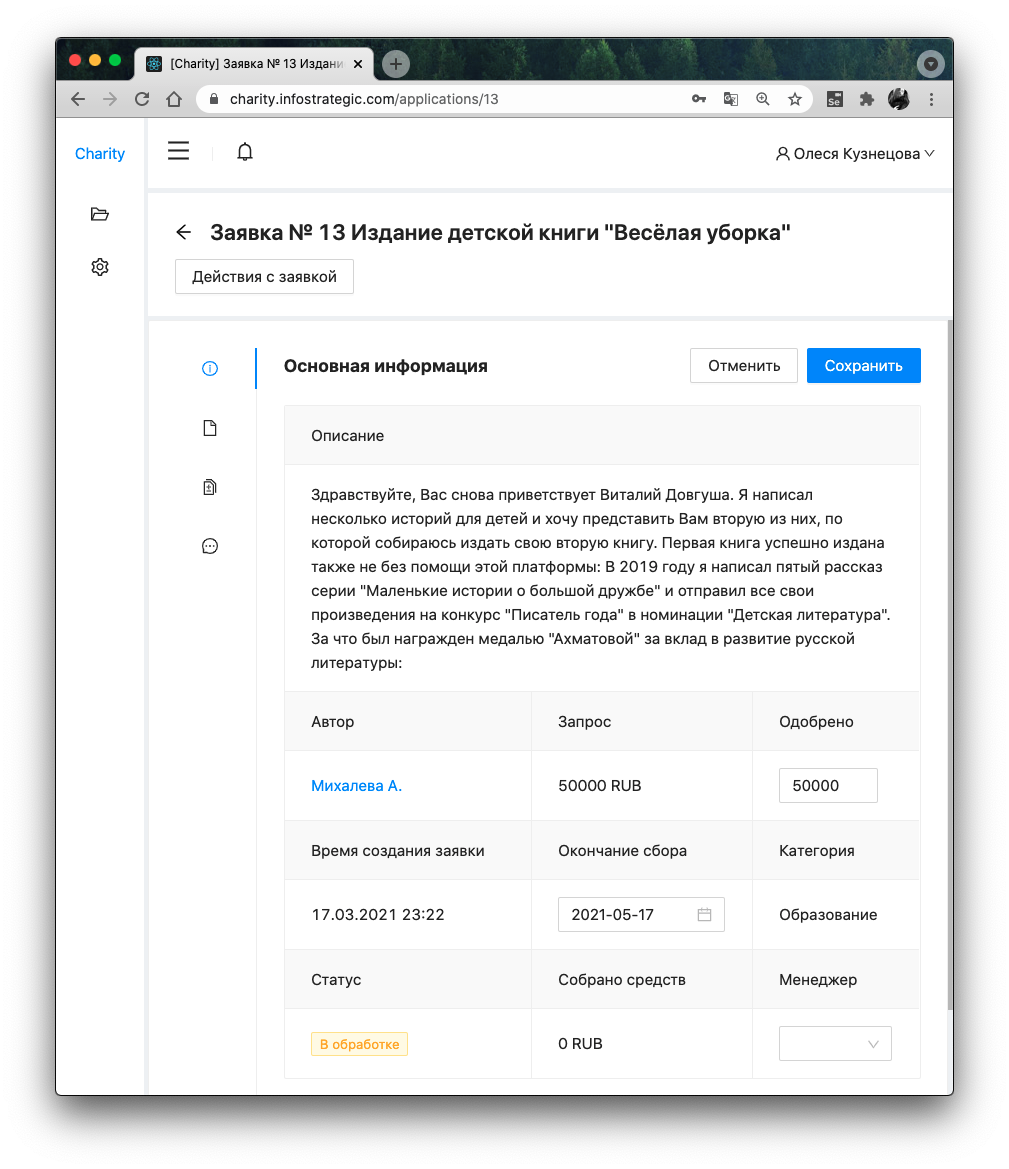
\includegraphics[width=\linewidth]{img/ro/application_edit.png}
		\end{subfigure}
		\begin{subfigure}[b]{0.475\linewidth}
			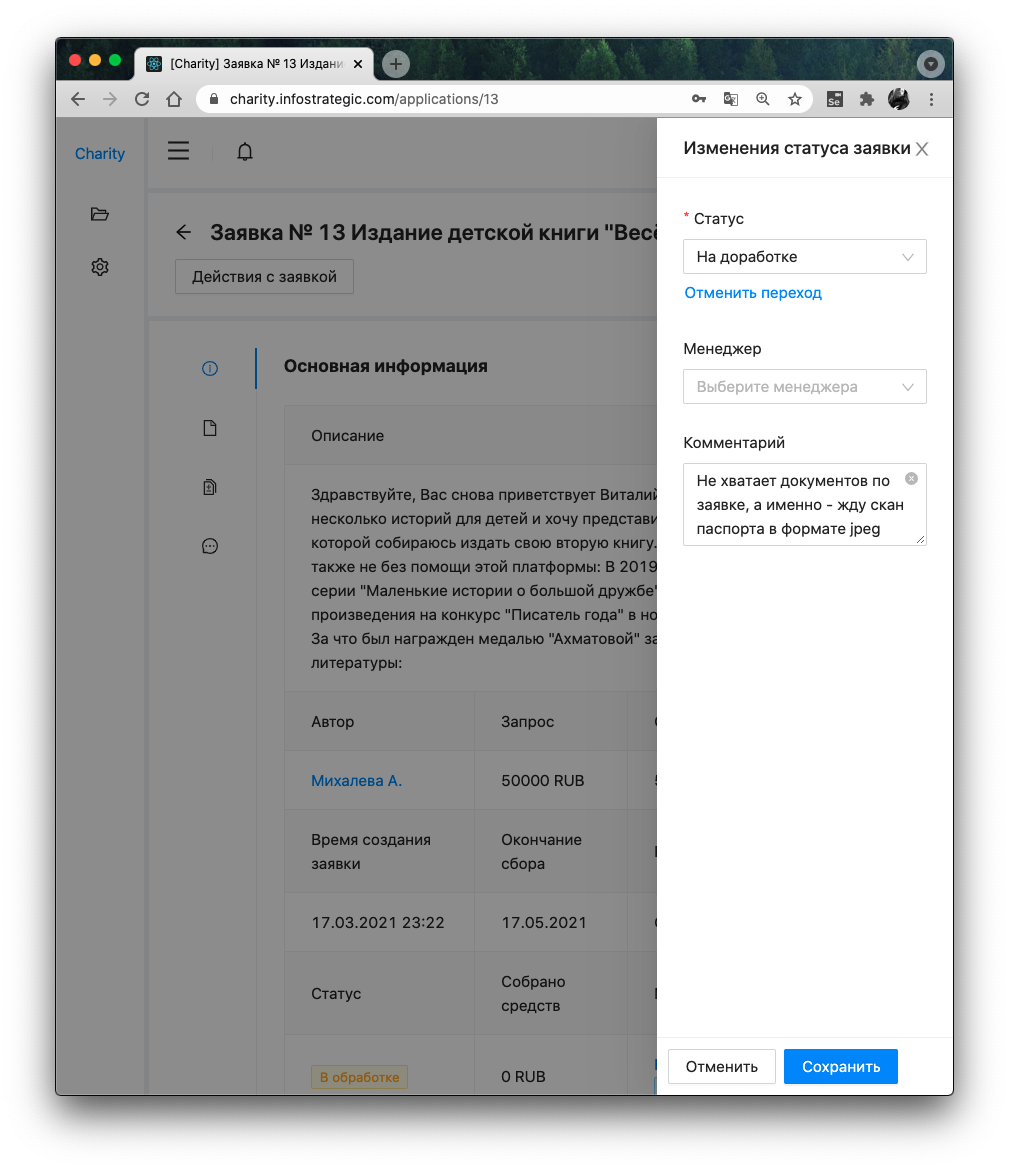
\includegraphics[width=\linewidth]{img/ro/application_drawer.png}
		\end{subfigure}
		\begin{subfigure}[b]{0.475\linewidth}
			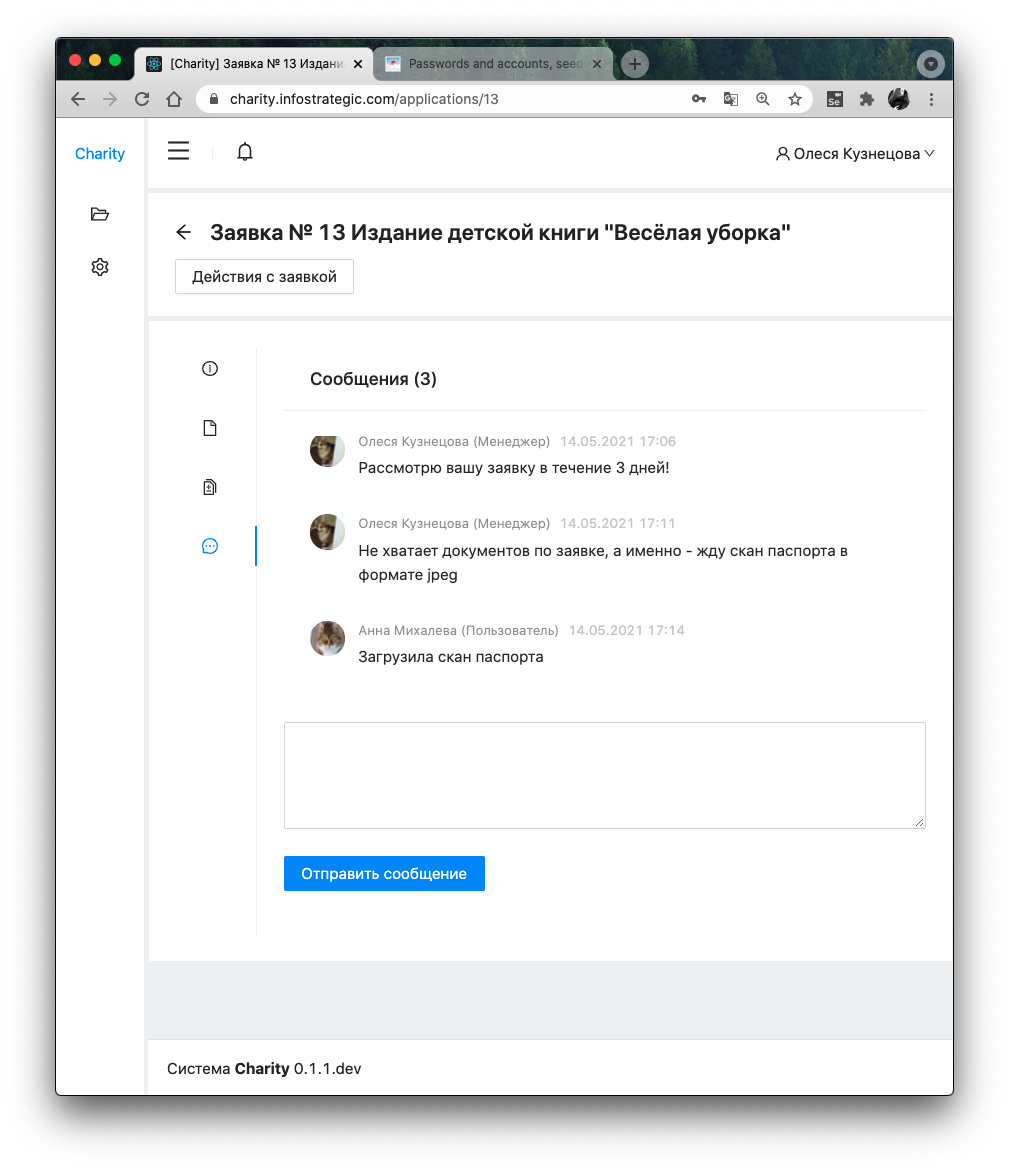
\includegraphics[width=\linewidth]{img/ro/application_comments.png}
		\end{subfigure}
		\caption{Скриншоты страницы заявки, менеджер}
		\label{pic: application_tabs}
	\end{figure}
	
	В табах, расположенных слева от описания заявки можно увидеть историю смены статусов заявки, а также комментарии. Результаты голосования можно увидеть в правой панели карточки, когда заявка находится в статусе <<Ждет подтверждения>> (от члена комиссии) (см. скриншот \ref{pic: application_tabs_1}).
		
	\begin{figure}[H]
	\centering
		\begin{subfigure}[b]{0.475\linewidth}
			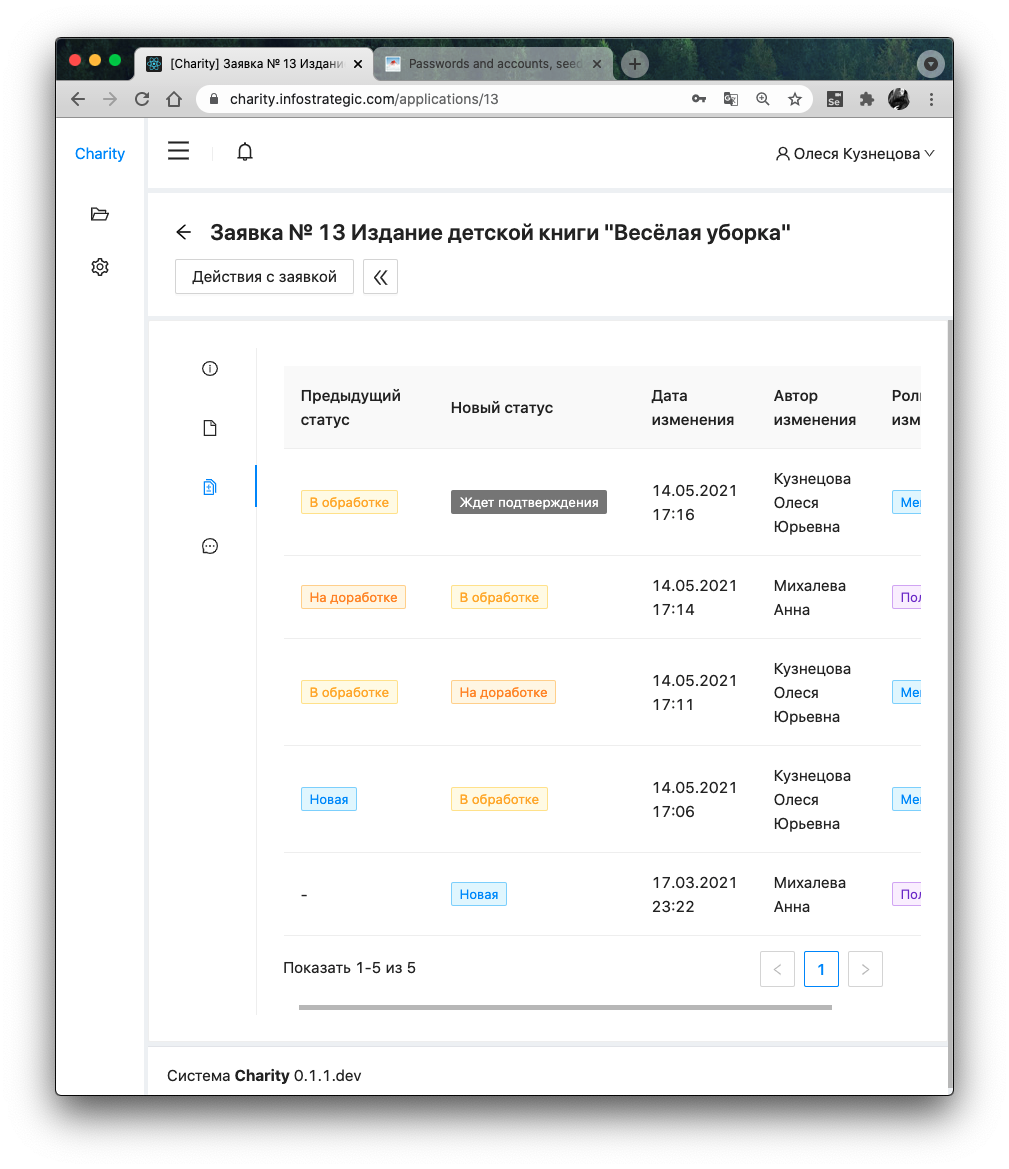
\includegraphics[width=\linewidth]{img/ro/application_history.png}
		\end{subfigure}
		\begin{subfigure}[b]{0.475\linewidth}
			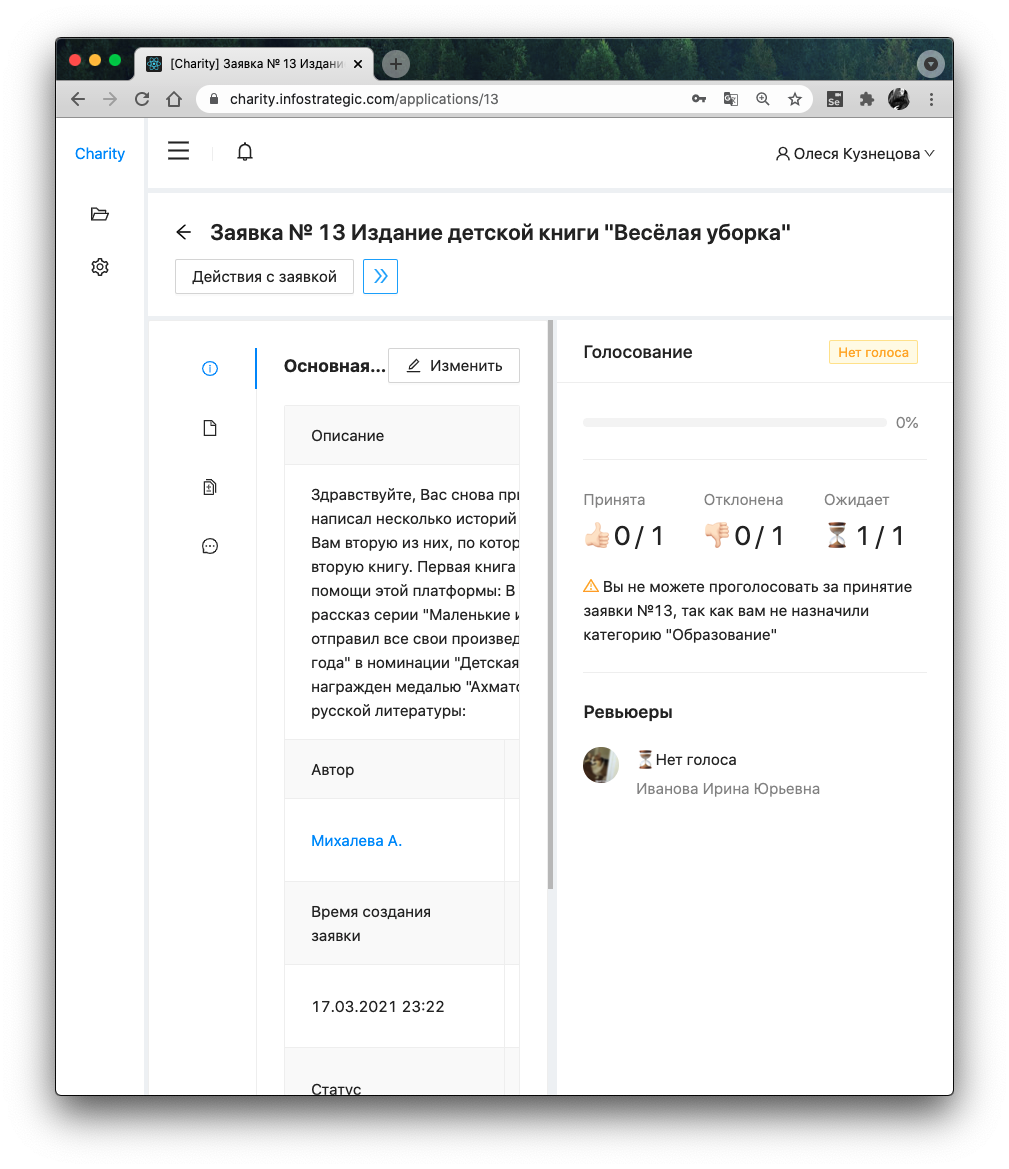
\includegraphics[width=\linewidth]{img/ro/application_m_vote.png}
		\end{subfigure}
		\caption{Скриншоты голосования и истории статусов заявки, менеджер}
		\label{pic: application_tabs_1}
	\end{figure}
	

    \subsubsection{Функционал члена комисии}
    
    При авторизации в системе пользователь с ролью <<Член комисии>> попадает на страницу авторизации с относительным url \texttt{/applications} со списком заявок на сбор средств, поступивших в систему (см. скриншоты \ref{pic: app_super}). Есть возможность отсортировать, а также отфильтровать заявки по статусу, по признаку назначена ли на данного члена комиссии заявка и требует ли она от него подтверждения.
    
    \begin{figure}[H]
	    \centering
		\begin{subfigure}[b]{0.475\linewidth}
			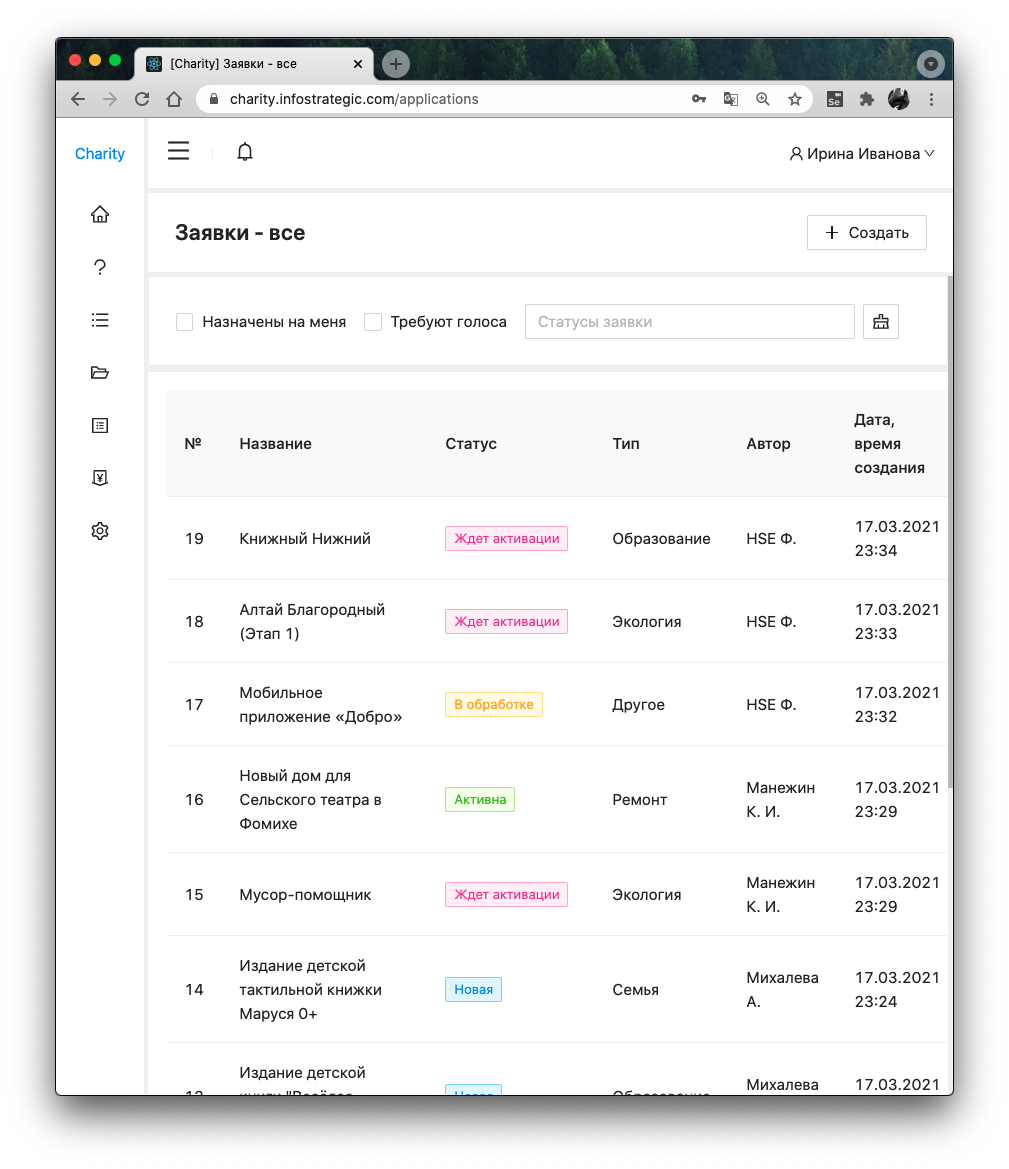
\includegraphics[width=\linewidth]{img/ro/app_super.png}
		\end{subfigure}
		\begin{subfigure}[b]{0.475\linewidth}
			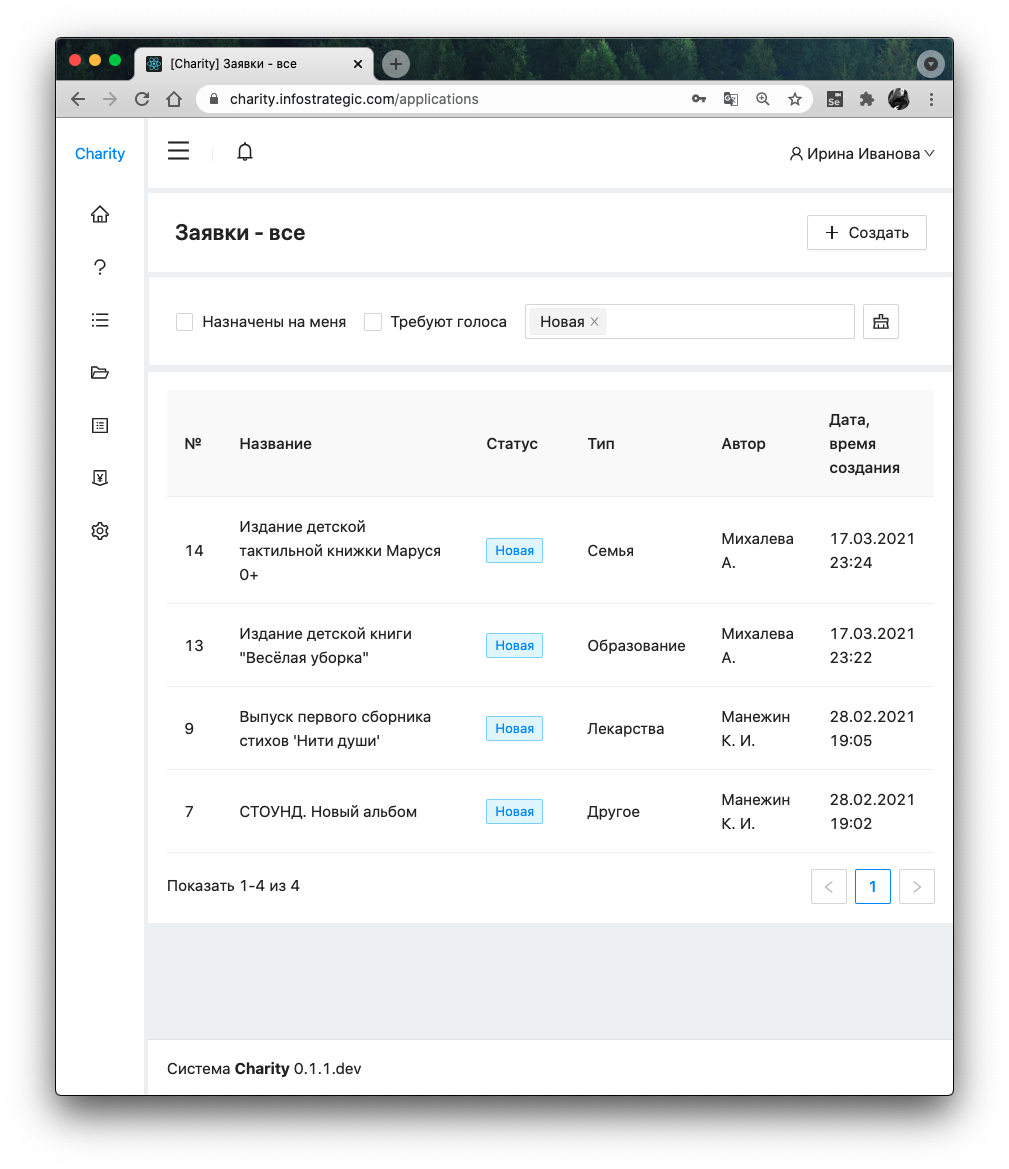
\includegraphics[width=\linewidth]{img/ro/app_super_filter.png}
		\end{subfigure}
		\caption{Скриншоты списка заявок, член комисии}
		\label{pic: app_super}
	\end{figure}
	
	При просмотре карточки заявки для члена комиссии доступна функциональность, аналогичная функционалу менеджера, описанного в разделе \ref{sec: man}. Остановимся на функциональности, не упомянутой в предыдущем разделе. У члена комиссии, назначенная категория которого (данную информацию о назначенных категориях можно посмотреть в настройках профиля, см. раздел \ref{sec: settings}) совпадает с категорией заявки, есть возможность проголосовать за активацию заявки. Процесс голосования изображен на скриншотах \ref{pic: vote}.
	
	
	\begin{figure}[H]
	    \centering
		\begin{subfigure}[b]{0.475\linewidth}
			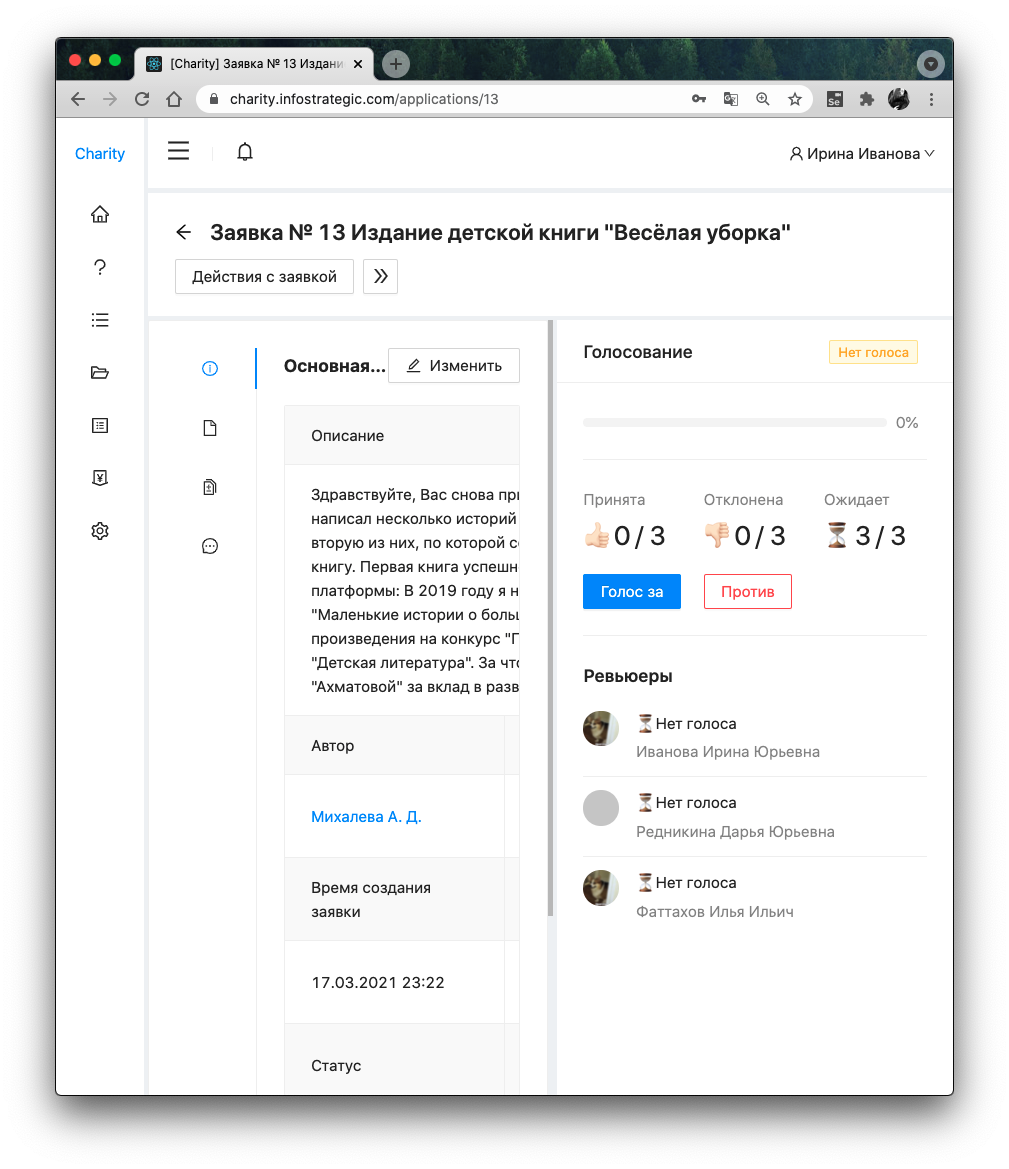
\includegraphics[width=\linewidth]{img/ro/not_voted.png}
		\end{subfigure}
		\begin{subfigure}[b]{0.475\linewidth}
			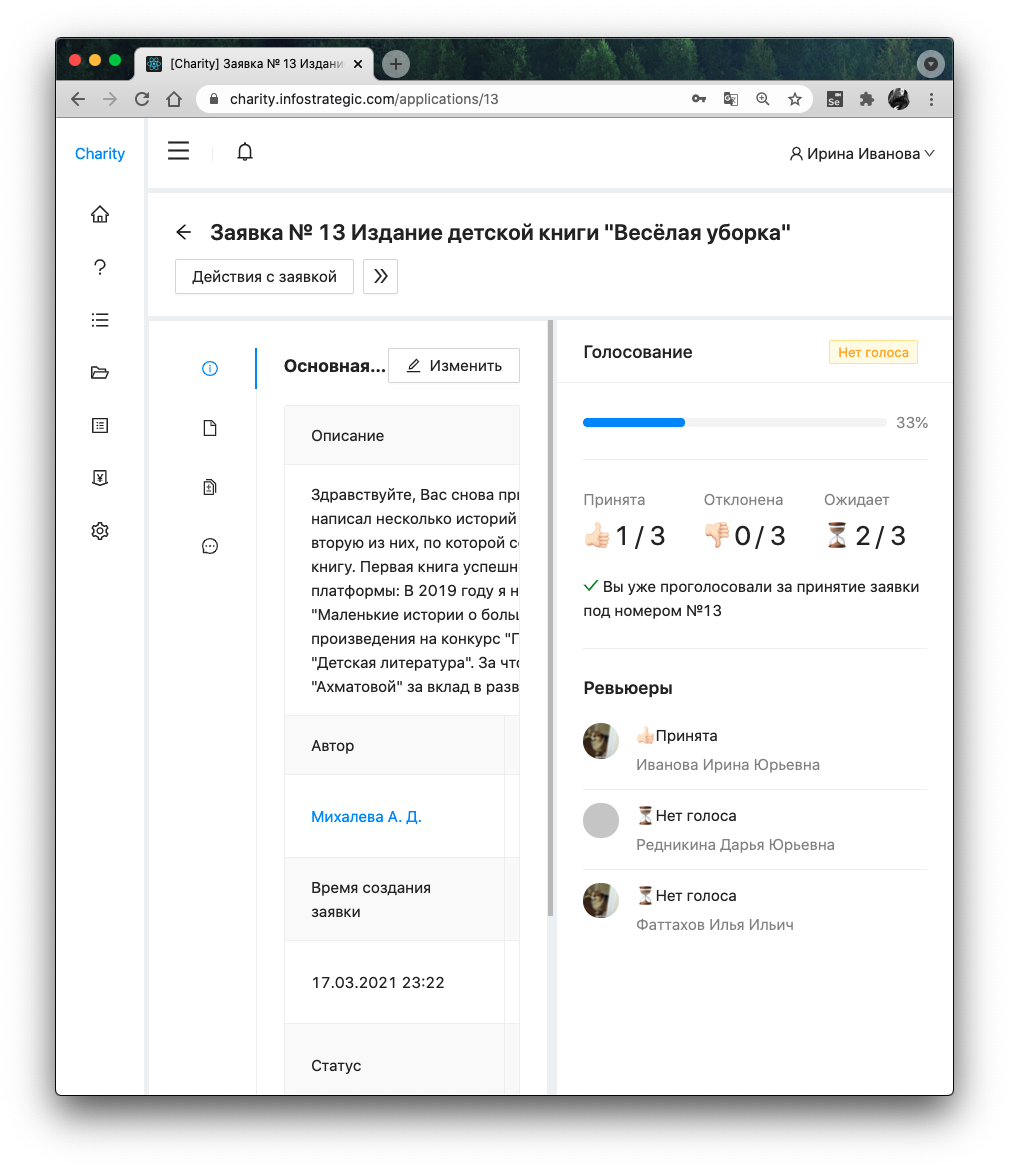
\includegraphics[width=\linewidth]{img/ro/vote_for.png}
		\end{subfigure}
		\begin{subfigure}[b]{0.475\linewidth}
			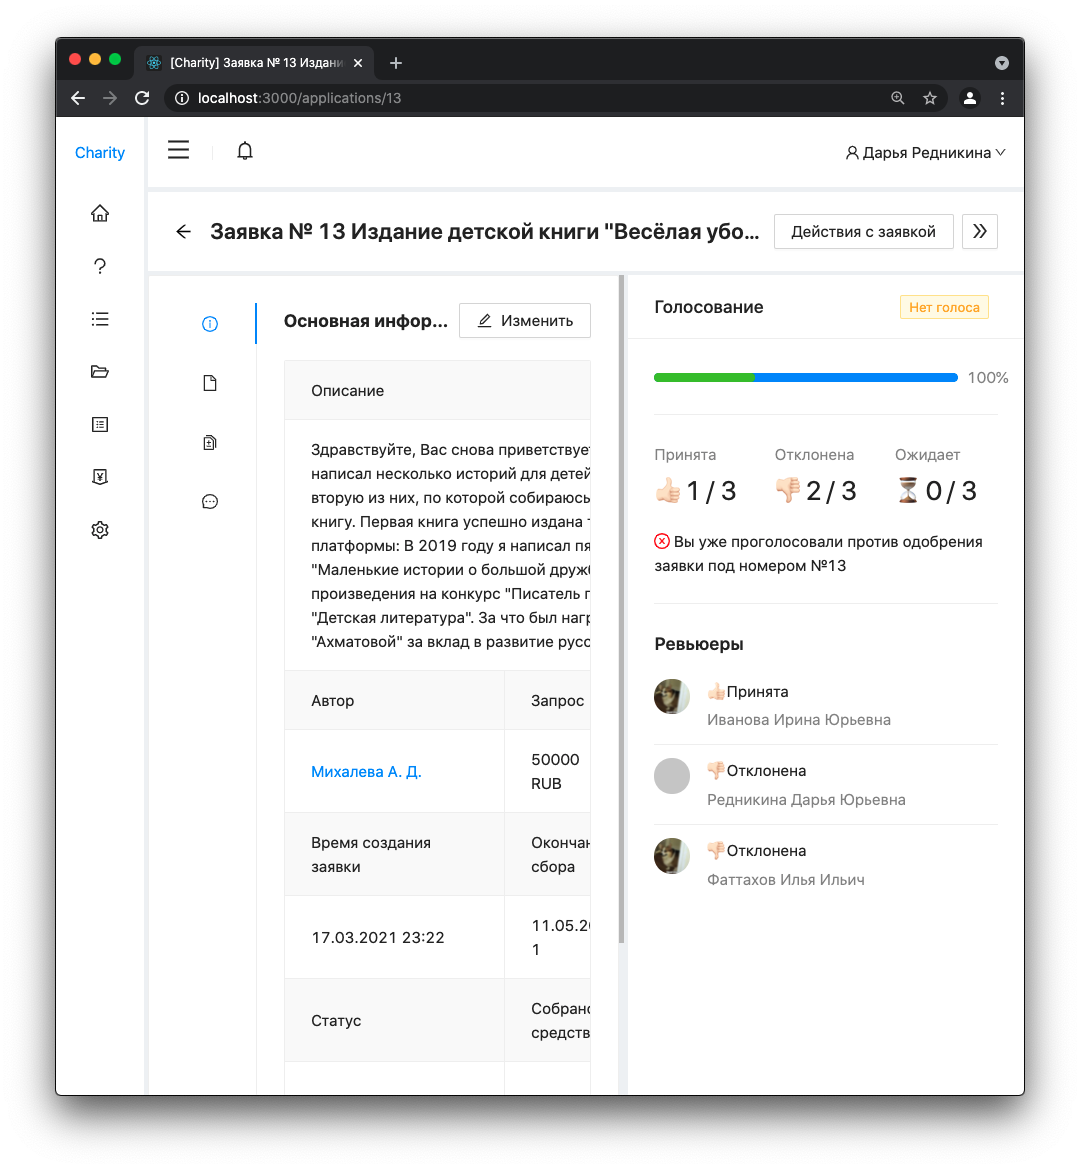
\includegraphics[width=\linewidth]{img/ro/vote_against.png}
		\end{subfigure}
		\begin{subfigure}[b]{0.475\linewidth}
			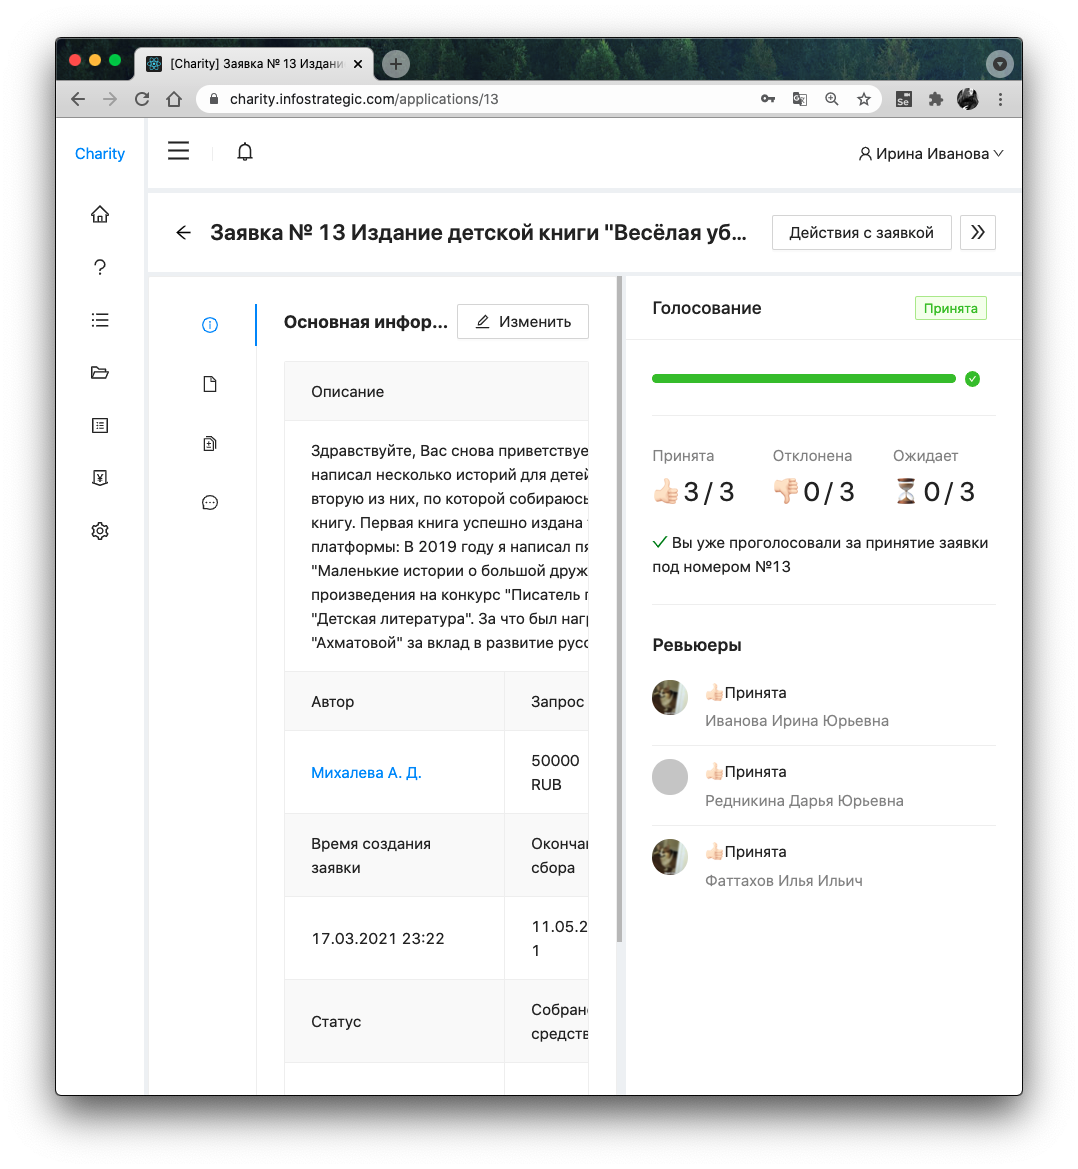
\includegraphics[width=\linewidth]{img/ro/vote_accepted.png}
		\end{subfigure}
		\caption{Скриншоты голосования за активацию заявки, член комисии}
		\label{pic: vote}
	\end{figure}
	
	После того, как голосование по заявке в статусе <<Ждет подтверждения>> завершено, ей можно поменять статус с помощью правой панели на <<Ждет активации>> (от пользователя). Таким образом, доведя ее до состояния активации (см. скриншоты \ref{pic: active}).
	
	\begin{figure}[H]
	    \centering
		\begin{subfigure}[b]{0.475\linewidth}
			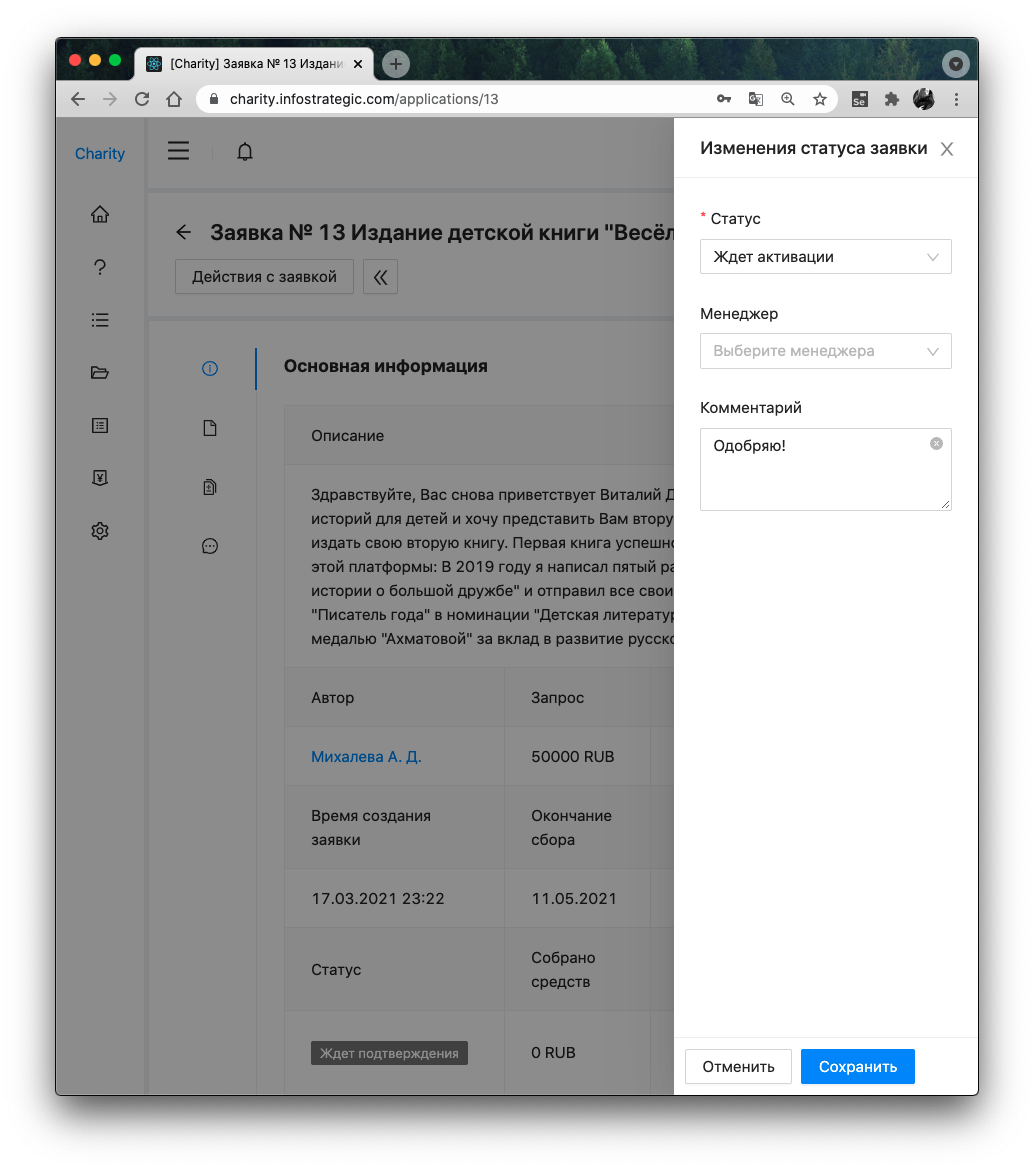
\includegraphics[width=\linewidth]{img/ro/activate.png}
		\end{subfigure}
		\begin{subfigure}[b]{0.475\linewidth}
			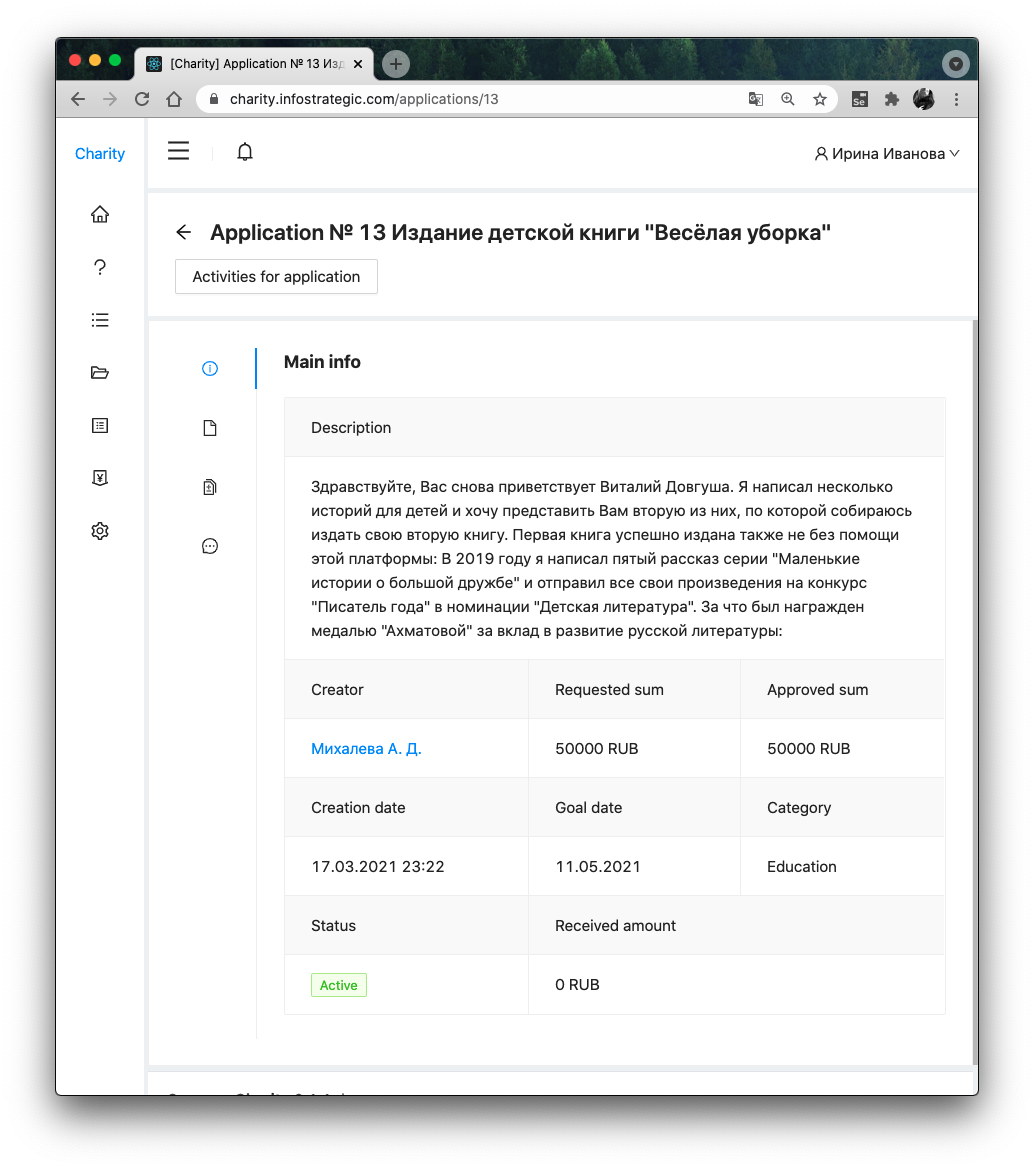
\includegraphics[width=\linewidth]{img/ro/active_page.png}
		\end{subfigure}
		\caption{Активирование заявки}
		\label{pic: active}
	\end{figure}
	
	Также член комисии имеет доступ к просмотру часто задаваемых вопросов к фонду по url \texttt{/faq} (или через меню в левой панели), см. скриншот \ref{pic: faq_super}. 
	
	\begin{figure}[H]
	    \centering
		\begin{subfigure}[b]{0.475\linewidth}
			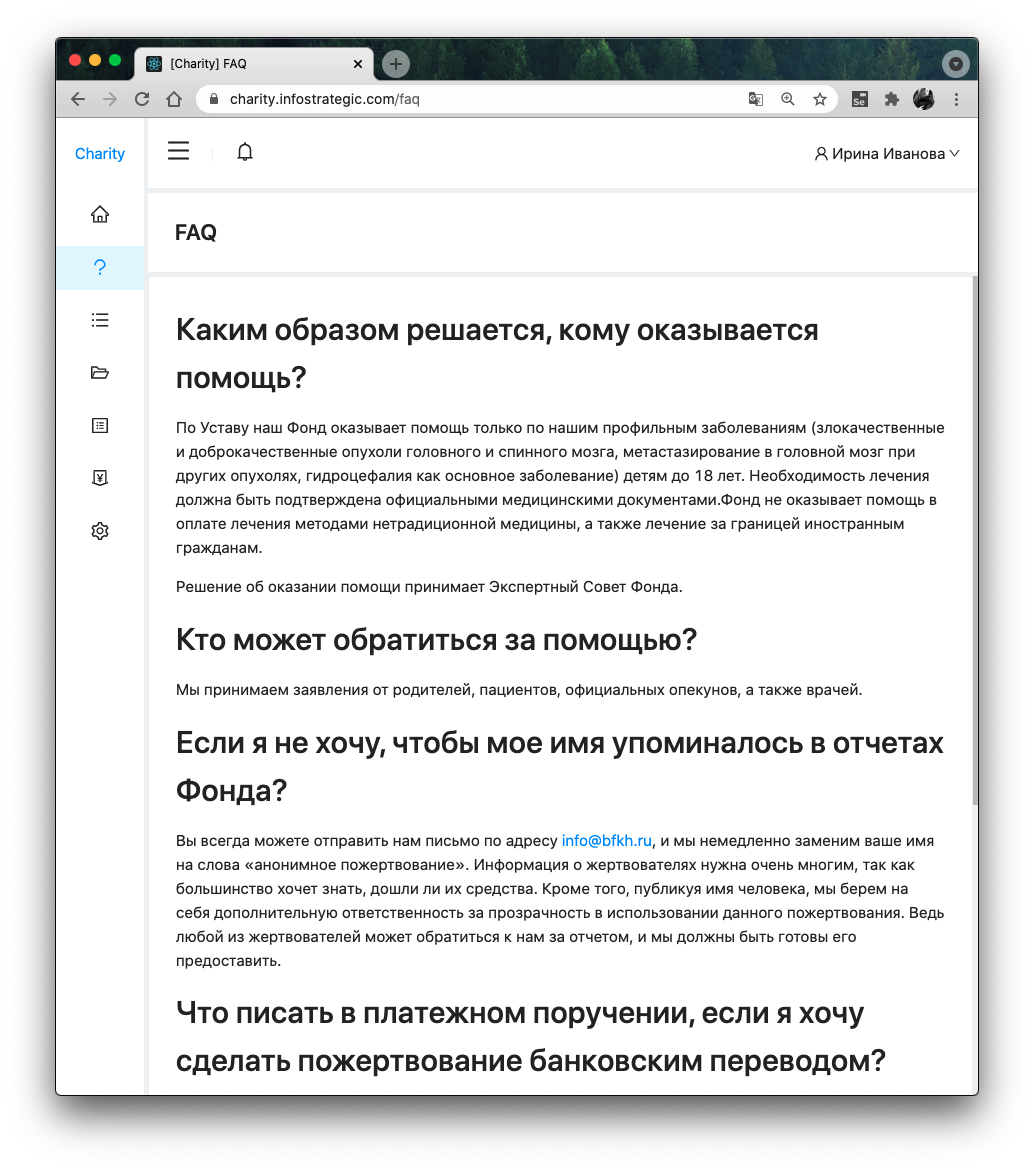
\includegraphics[width=\linewidth]{img/ro/faq_super.png}
		\end{subfigure}
		\caption{Просмотр FAQ}
		\label{pic: faq_super}
	\end{figure}
	
	Также у члена комисии есть доступ к странице со списком категорий по адресу \texttt{/categories} или по клику в левом навигационном меню, с возможностью просмотра списка и его редактирования (см. скриншоты \ref{pic: categories}). По кнопке <<Подтвердить изменения>> сохраняются внесенные изменения в указанные категории. 
	
	\begin{figure}[H]
	    \centering
		\begin{subfigure}[b]{0.475\linewidth}
			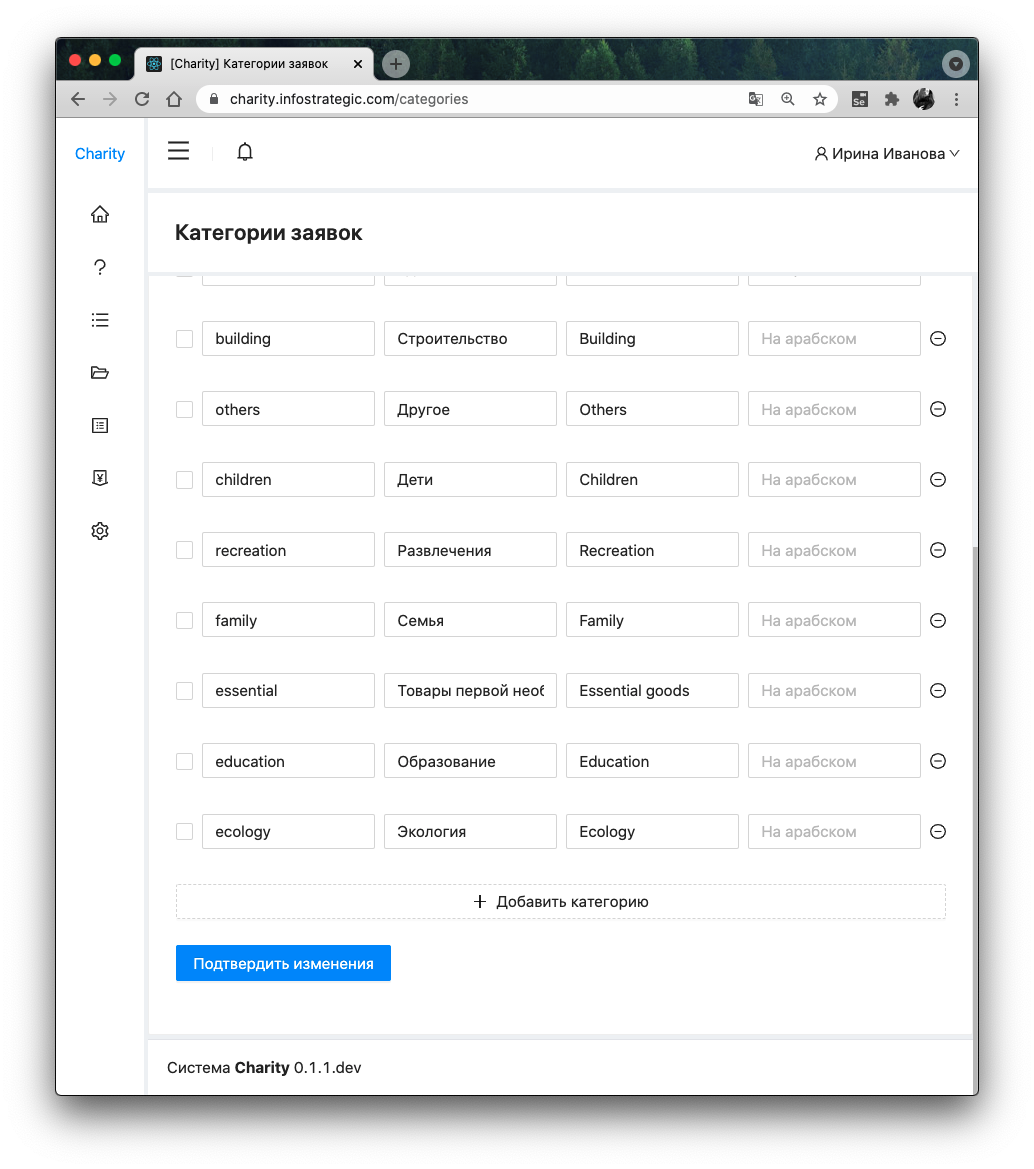
\includegraphics[width=\linewidth]{img/ro/categories.png}
		\end{subfigure}
		\caption{Скриншот просмотра и редактирования категорий}
		\label{pic: categories}
	\end{figure}
	
	У члена комисии есть доступ к странице со списком менеджеров фонда по адресу \texttt{/managers} или по клику в левом навигационном меню, с возможностью просмотра списка и его фильтрации (см. скриншоты \ref{pic: managers}). Перейдя на страницу сотрудника можно увидеть над какими заявками он сейчас работает и информацию о нем.
	
	\begin{figure}[H]
	    \centering
		\begin{subfigure}[b]{0.475\linewidth}
			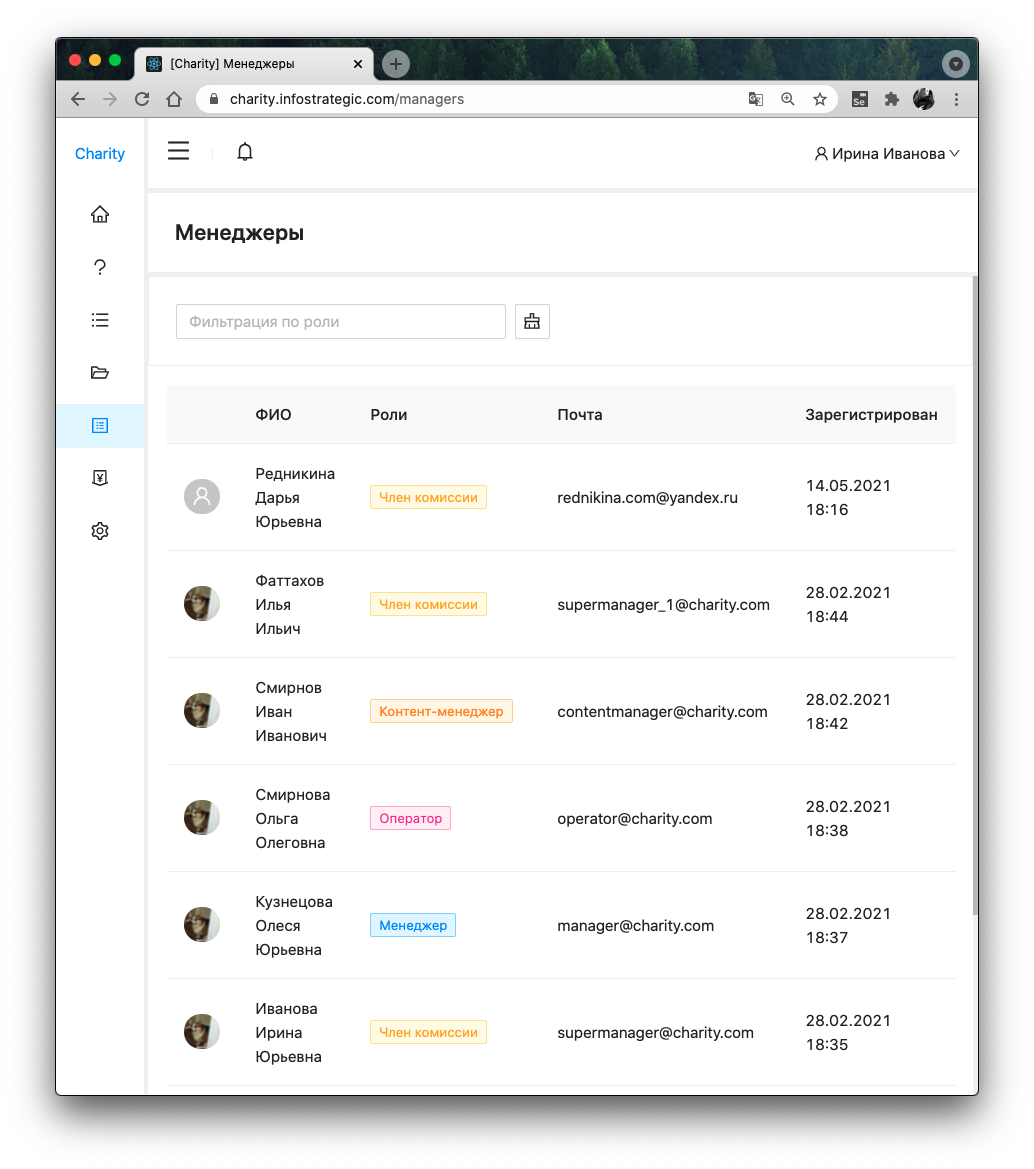
\includegraphics[width=\linewidth]{img/ro/managers.png}
		\end{subfigure}
		\begin{subfigure}[b]{0.475\linewidth}
			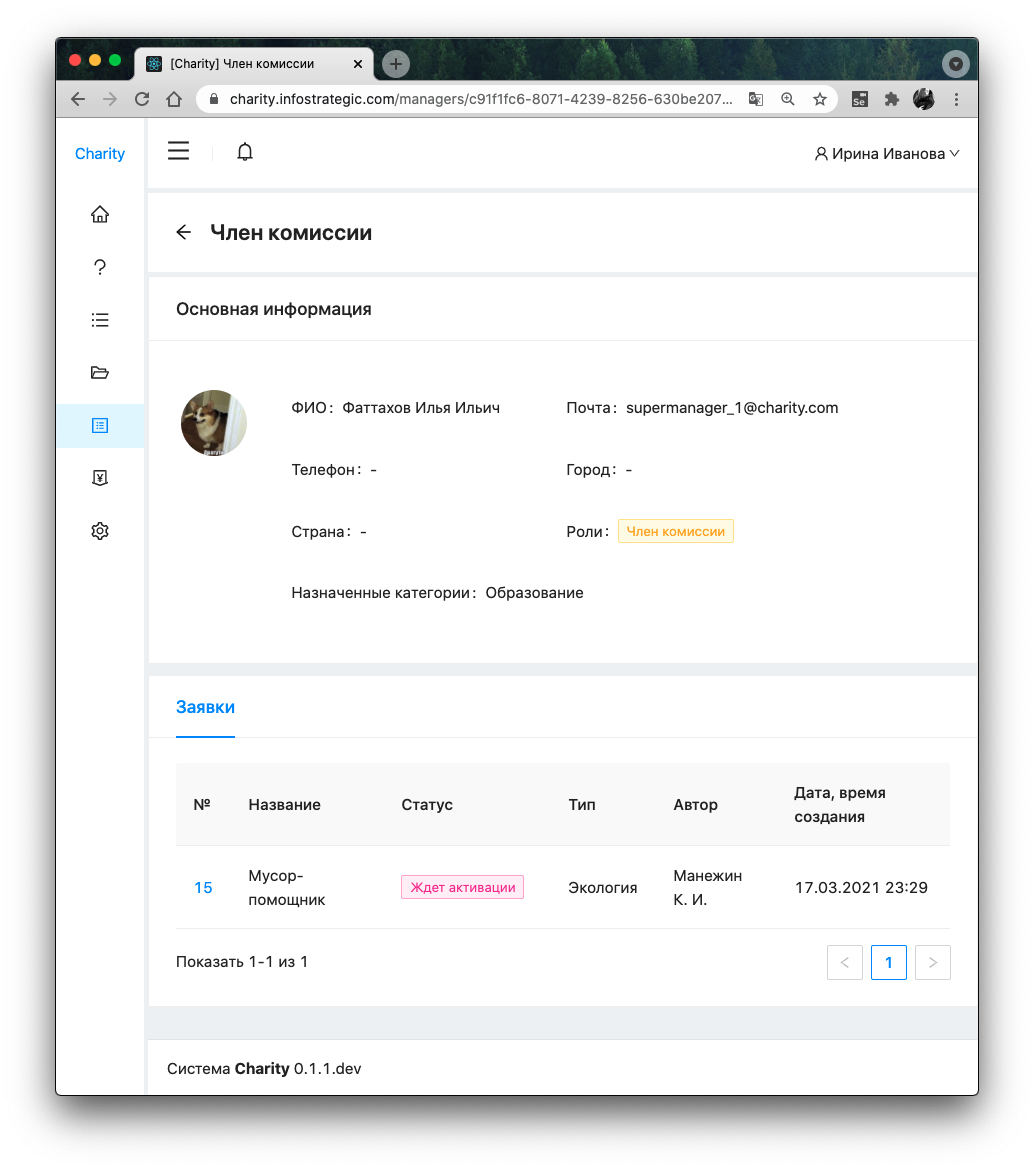
\includegraphics[width=\linewidth]{img/ro/manager_page.png}
		\end{subfigure}
		\caption{Скриншоты списка менеджеров фонда и просмотра информации о них}
		\label{pic: managers}
	\end{figure}
	
   У члена комисии есть доступ к странице со списком пожертвований фонда по адресу \texttt{/transactions} или по клику в левом навигационном меню, с возможностью просмотра списка транзакций (см. скриншоты \ref{pic: transactions}). 
    
    \begin{figure}[H]
	    \centering
		\begin{subfigure}[b]{0.475\linewidth}
			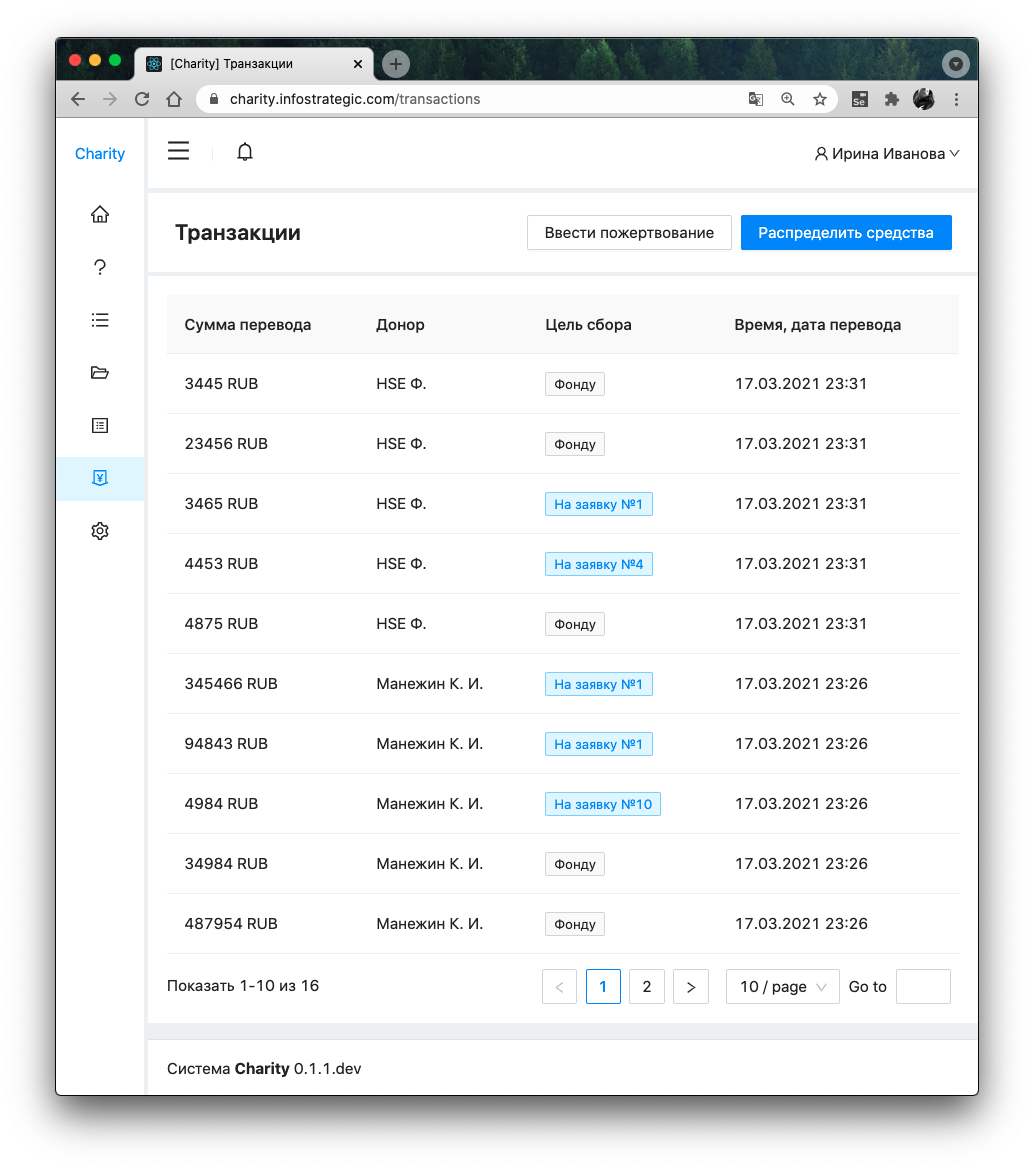
\includegraphics[width=\linewidth]{img/ro/transactions.png}
		\end{subfigure}
		\begin{subfigure}[b]{0.475\linewidth}
			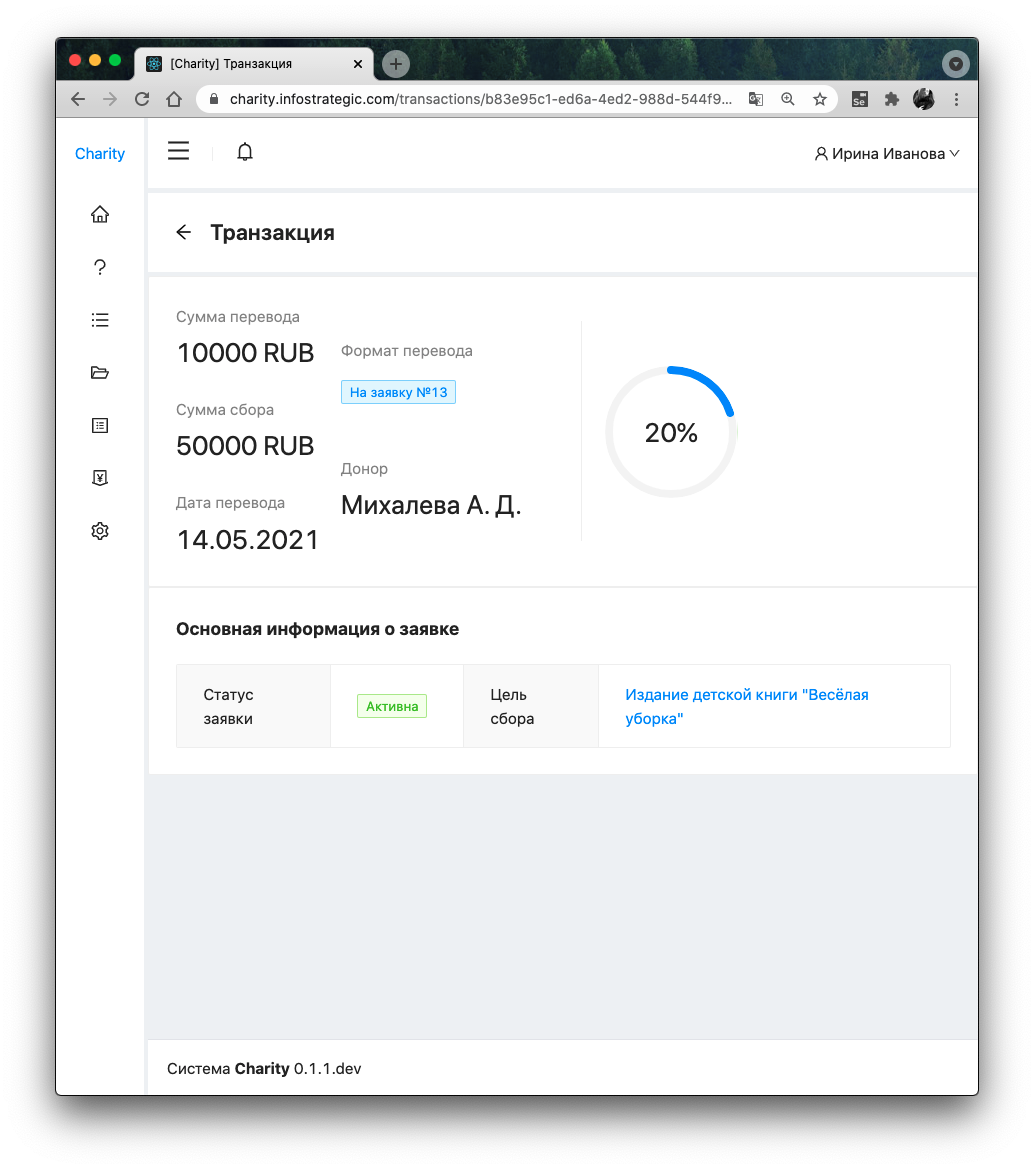
\includegraphics[width=\linewidth]{img/ro/donation.png}
		\end{subfigure}
		\caption{Скриншоты списка транзакции и просмотра информации об одной из них}
		\label{pic: transactions}
	\end{figure}
	
	По кнопке <<Ввести пожертвование>> можно зарегистрировать пожертвование, поступившее в Фонд напрямую от донора, не через систему. Введя базовые данные в форму пожертвование регистрируется от имени самого фонда (см. скриншоты \ref{pic: manual_donation}). 
	
	\begin{figure}[H]
	    \centering
		\begin{subfigure}[b]{0.475\linewidth}
			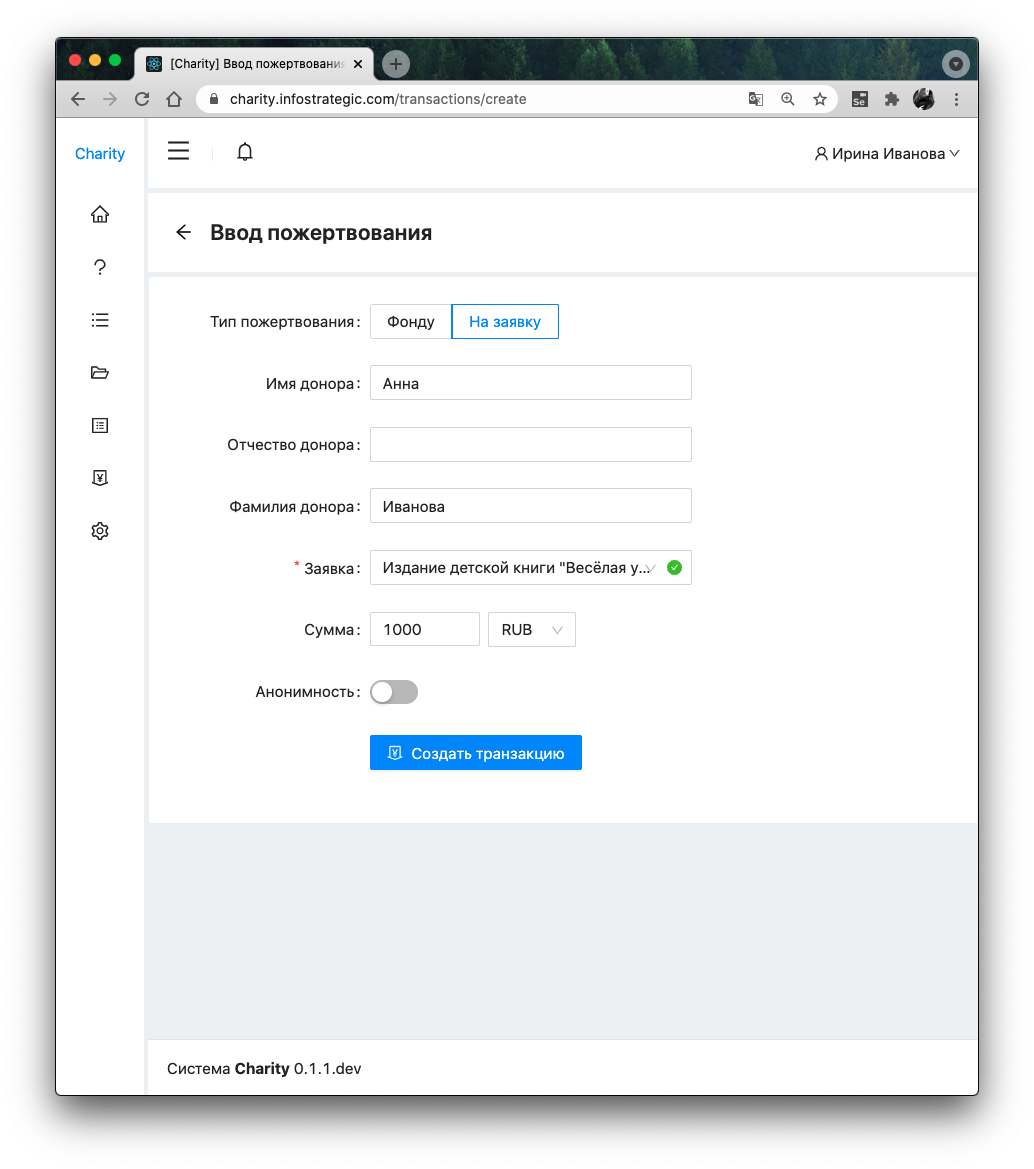
\includegraphics[width=\linewidth]{img/ro/donation_manual.png}
		\end{subfigure}
		\begin{subfigure}[b]{0.475\linewidth}
			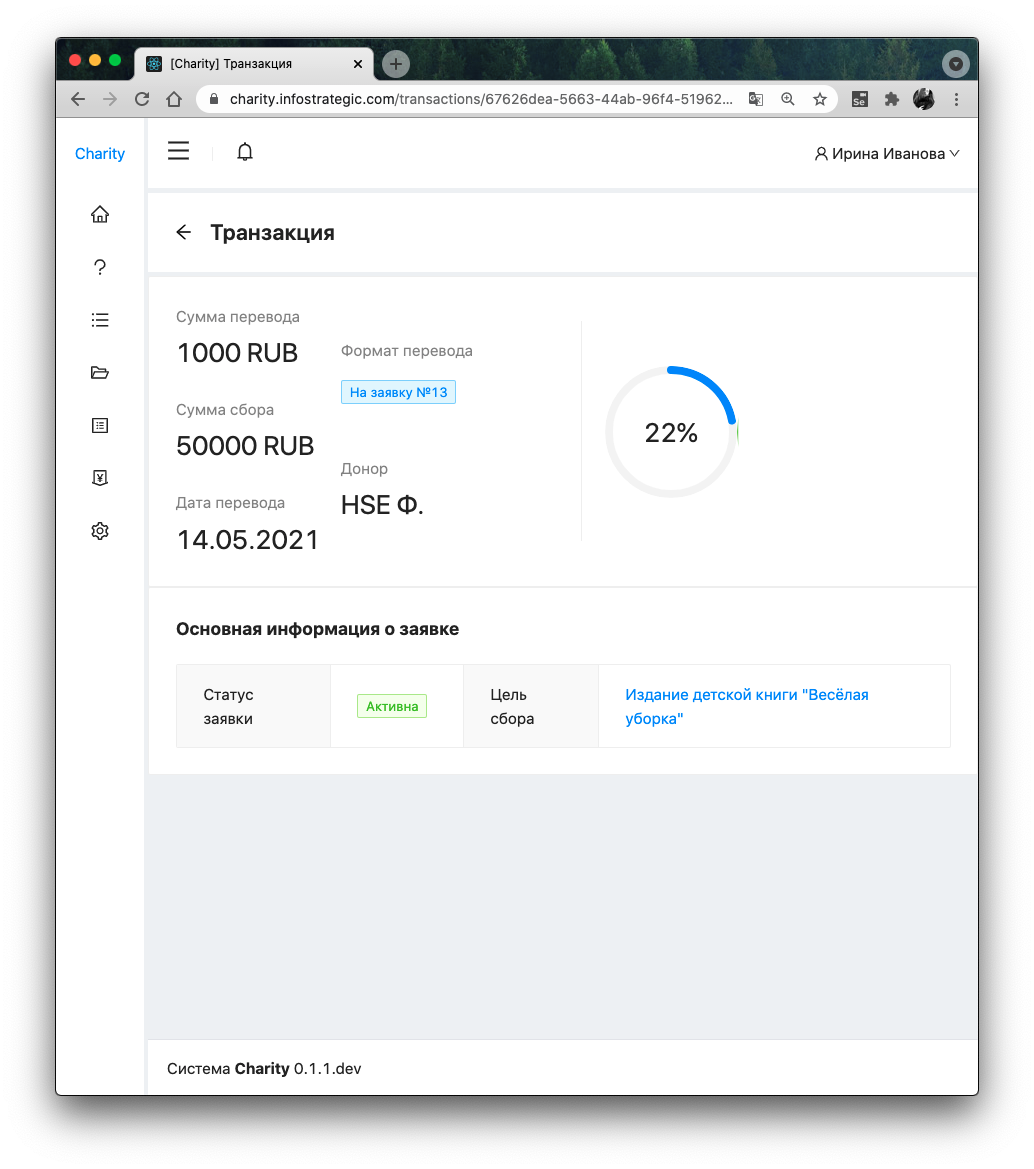
\includegraphics[width=\linewidth]{img/ro/donation_from_fund.png}
		\end{subfigure}
		\caption{Скриншоты регистрации ручной заявки}
		\label{pic: manual_donation}
	\end{figure}
	
	По кнопке <<Распределить средства>> можно распределить средства с баланса фонда напрямую заявке. Введя данные заявки и сумму можно совершить пожертвование от имени фонда (см. скриншоты \ref{pic: distribute}). 
	
		\begin{figure}[H]
	    \centering
		\begin{subfigure}[b]{0.475\linewidth}
			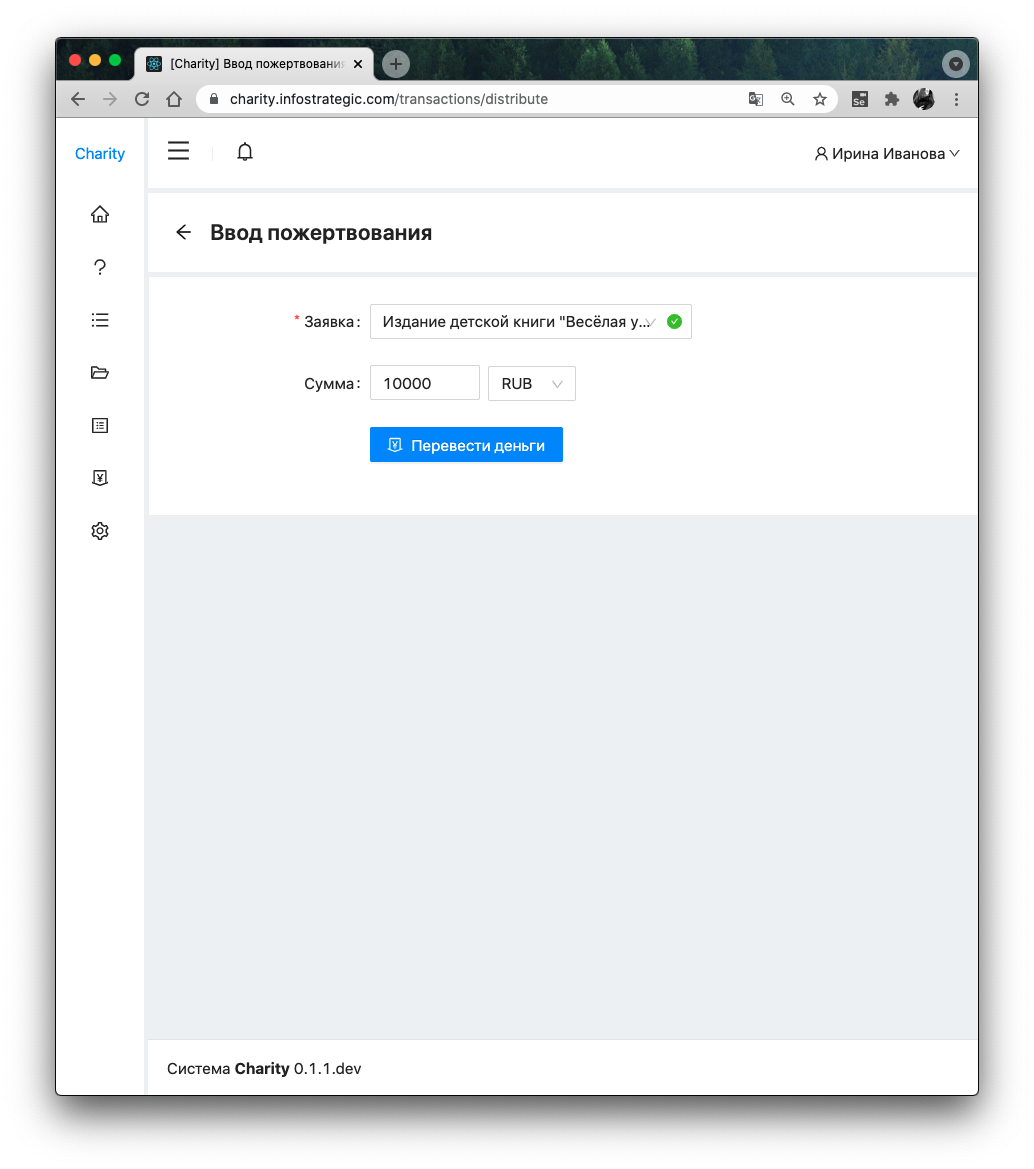
\includegraphics[width=\linewidth]{img/ro/donation_distribute_form.png}
		\end{subfigure}
		\begin{subfigure}[b]{0.475\linewidth}
			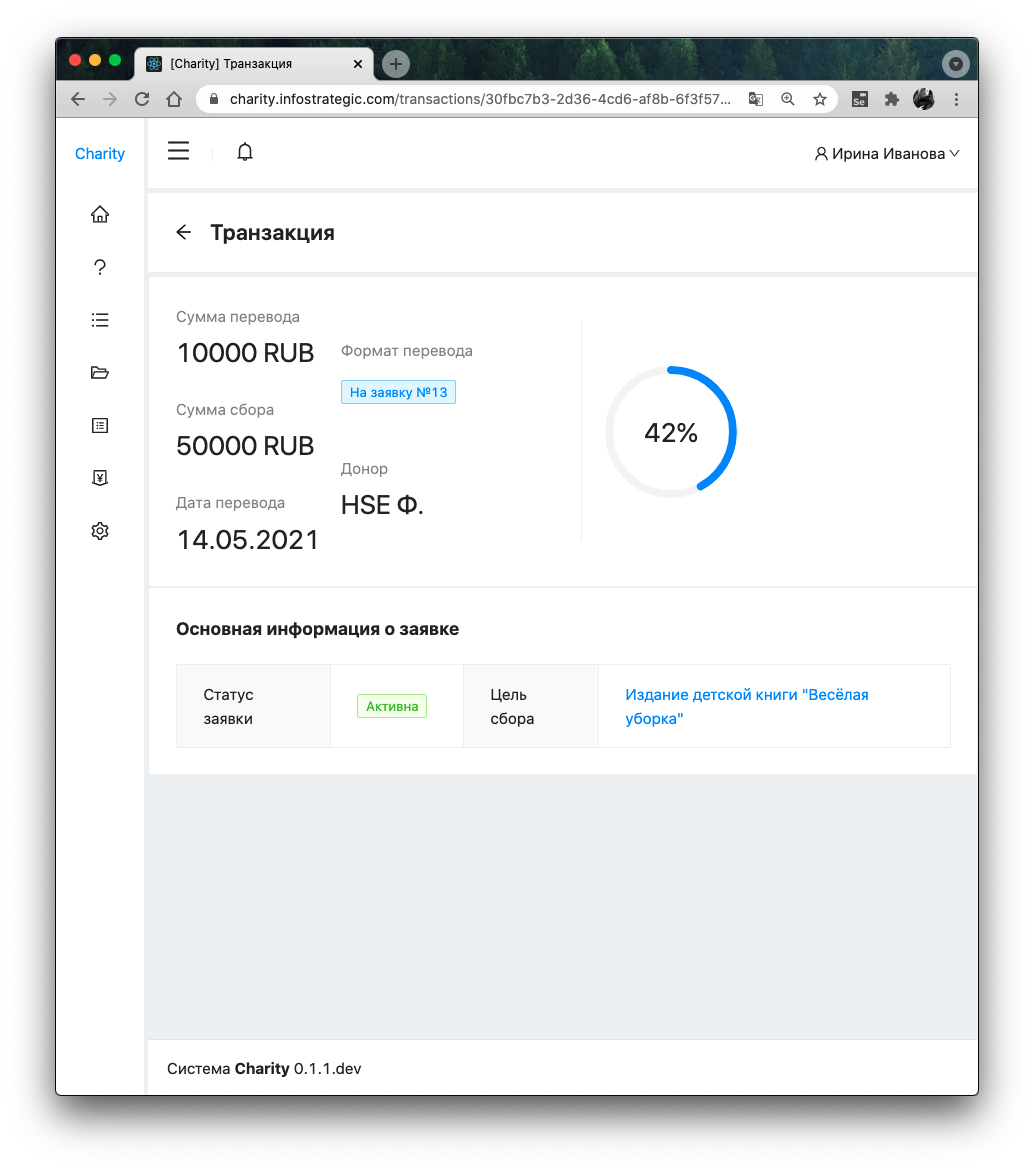
\includegraphics[width=\linewidth]{img/ro/donation_distribute.png}
		\end{subfigure}
		\caption{Скриншоты распределения средств}
		\label{pic: distribute}
	\end{figure}
     
	\subsubsection{Функционал оператора}
	
	При авторизации в приложении пользователи с ролью <<Оператор>> попадают на страницу со списком диалогов с относительным адресом \texttt{/chats}. У операторов есть возможность перейти в чат с пользователем и ответить на его/ее сообщения (см. скриншоты \ref{pic: chats}). 
	
	\begin{figure}[H]
	    \centering
		\begin{subfigure}[b]{0.475\linewidth}
			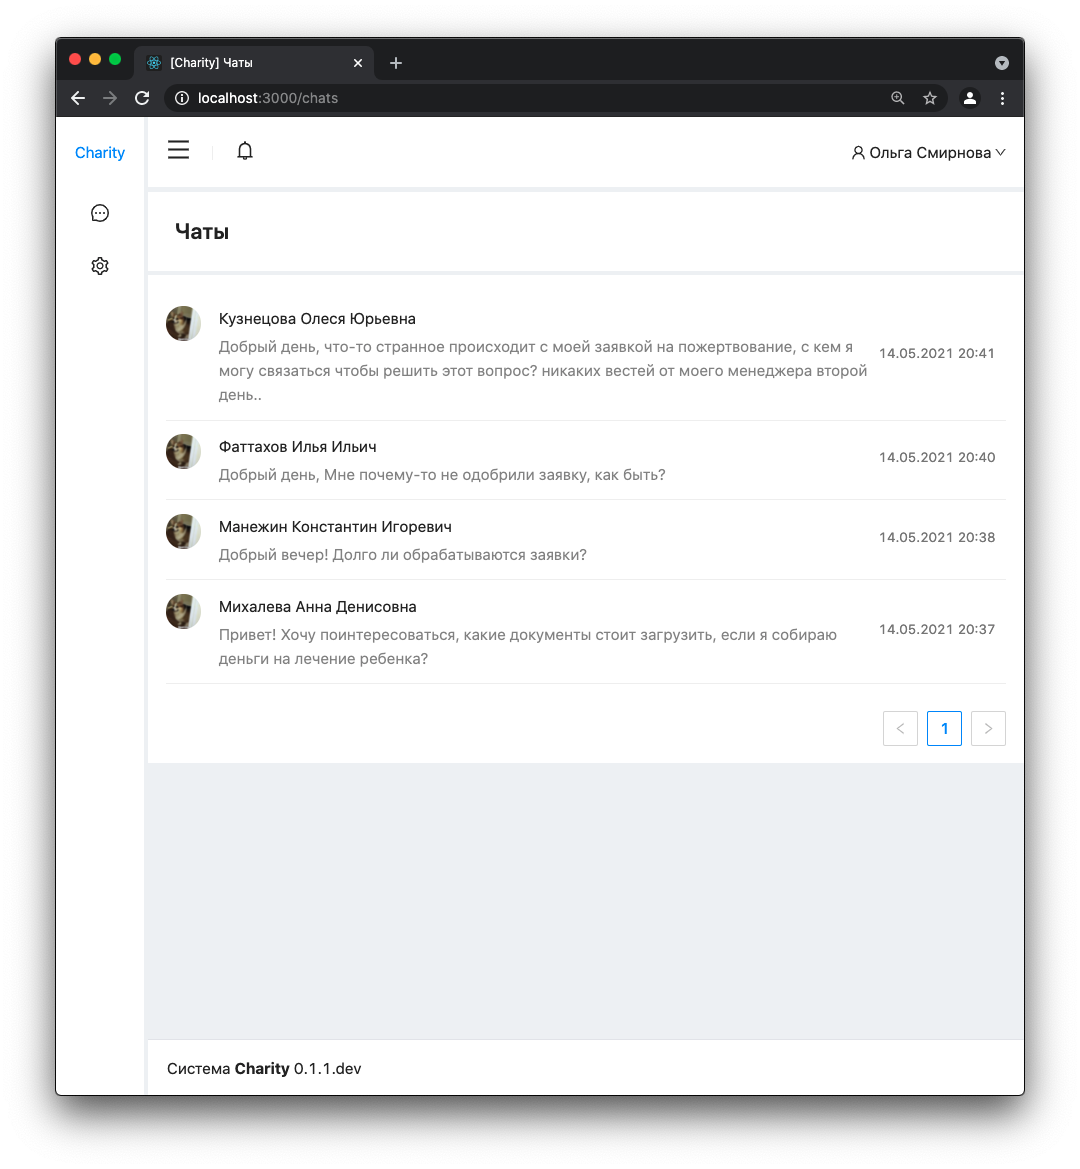
\includegraphics[width=\linewidth]{img/ro/chats.png}
		\end{subfigure}
		\begin{subfigure}[b]{0.475\linewidth}
			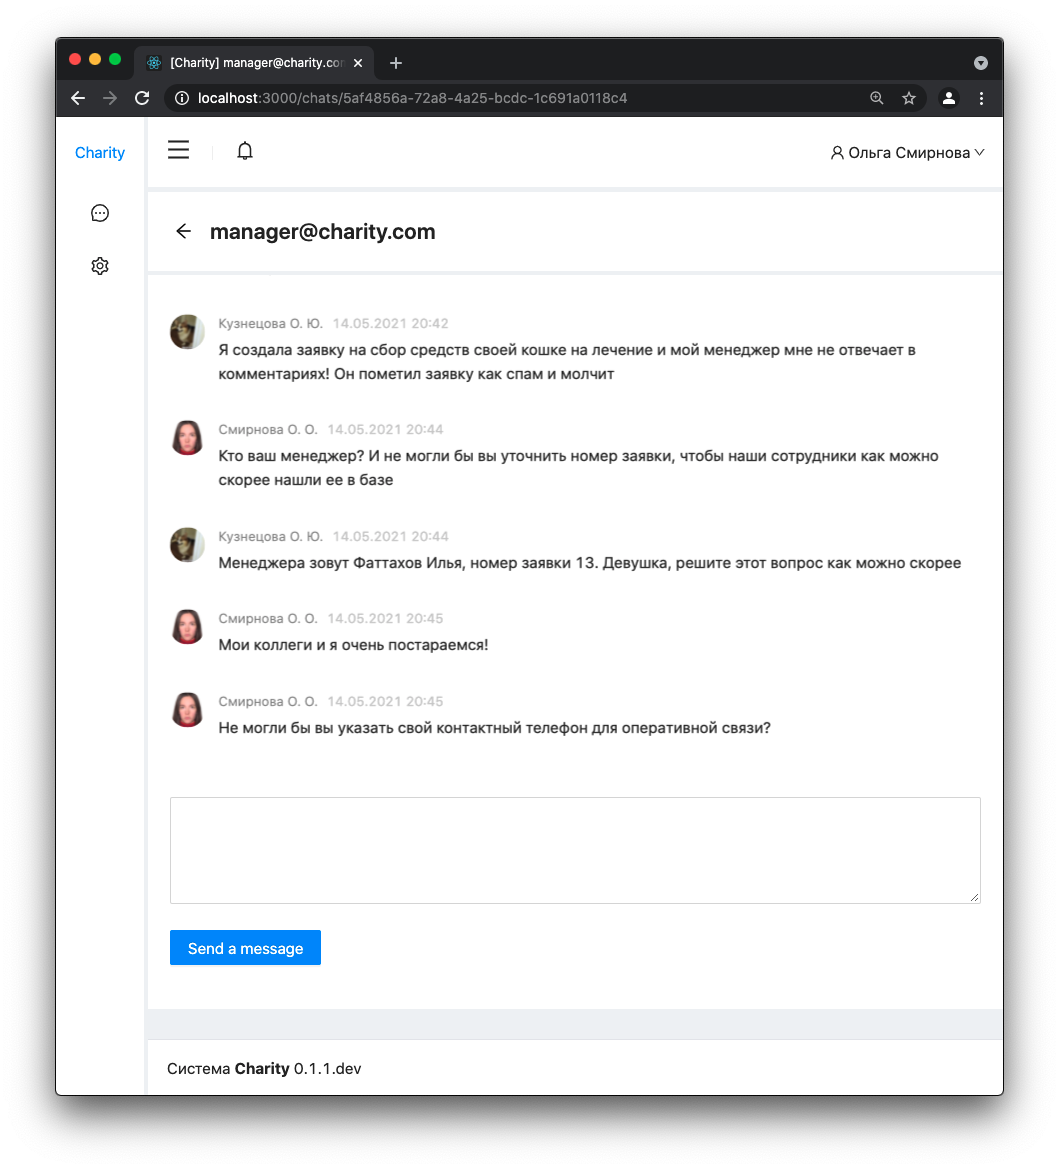
\includegraphics[width=\linewidth]{img/ro/one_chat.png}
		\end{subfigure}
		\caption{Скриншоты чатов с пользователями}
		\label{pic: chats}
	\end{figure}
	
	\subsubsection{Выход из приложения}
	
	Для пользователей с любой ролью выход из приложения доступен через хэдер и выпадающее меню в правом верхнем углу (см. скриншот \ref{pic: logout} и выделенную красным область).
	
	
	\begin{figure}[H]
	    \centering
		\begin{subfigure}[b]{0.475\linewidth}
			\includegraphics[width=\linewidth]{img/ro/logout.png}
		\end{subfigure}
		\caption{Скриншот выхода из приложения}
		\label{pic: logout}
	\end{figure}
	
	\section{Сообщения оператору}
	
	При незаполнении форм в системе с обязательными полями, система выводит предупреждающее сообщение под каждым из незаполненных полей (см. скриншоты \ref{pic: form_obl}).
	
	\begin{figure}[h!]
		\centering
		\begin{subfigure}[b]{0.35\linewidth}
			\includegraphics[width=\linewidth]{img/ro/login_error_password.png}
			\caption{\label{pic: invalid_login} Незаполненный пароль в форме авторизации}
		\end{subfigure}
		\begin{subfigure}[b]{0.35\linewidth}
			\includegraphics[width=\linewidth]{img/ro/create_application_form.png}
			\caption{\label{pic: success} Незаполенные обязетальные поля в форме создания заявки}
		\end{subfigure}
		\caption{\label{pic: form_obl} Сообщения оператору, подписи в форме}
	\end{figure}
	
	При успехе, ошибке совершенной операции (например, при попытке авторизоваться - см. скриншот \ref{pic: invalid}) система отображает уведомление в левом нижнем углу с текстом описания совершенной операции/выявленной проблемы. При получении уведомления с красным фоном стоит повторить попытку. Примеры других уведомлений можно увидеть на скриншотах \ref{pic: wr}.
	
	\begin{figure}[h!]
		\centering
		\begin{subfigure}[b]{0.3\linewidth}
			\includegraphics[width=\linewidth]{img/ro/login_error.png}
			\caption{\label{pic: invalid} Неверный логин и пароль}
		\end{subfigure}
		\begin{subfigure}[b]{0.3\linewidth}
			\includegraphics[width=\linewidth]{img/ro/reg_success.png}
			\caption{\label{pic: success} Уведомление об успехе совершенной операции}
		\end{subfigure}
		\begin{subfigure}[b]{0.315\linewidth}
			\includegraphics[width=\linewidth]{img/ro/info.png}
			\caption{\label{pic: wrong_code} Уведомление об отмене операции}
		\end{subfigure}
		\caption{\label{pic: wr} Сообщения оператору, уведомления}
	\end{figure}
	
	Так как в системе используются пуш-уведомления для оповещения о совершенных операциях, то соответствующие нотификации появляются в верхнем правом углу. Пуш-уведомления приходят при смене статуса заявки, которую обрабатывает менеджер, а также оператору при получении новых сообщений (см. скриншот \ref{pic: firebase}).
	
	\begin{figure}[H]
		\centering
		\begin{subfigure}[b]{0.45\linewidth}
			\includegraphics[width=\linewidth]{img/ro/push.png}
			\caption{\label{pic: firebase_push} Уведомление о смене статуса заявки}
		\end{subfigure}
		\caption{\label{pic: firebase} Сообщения оператору, пуш-уведомления}
	\end{figure}
	
	\newpage
	%\section{Источники, использованные при разработке}
	%\renewcommand{\refname}{Список источников}
	% \addcontentsline{toc}{subsection}{\refname}
	\patchcmd{\thebibliography}{\section*{\refname}}{}{}{}
	\anonsection{Список источников}
	\begin{thebibliography}{3}
		\bibitem{gost}Единая система программной документации – М.: ИПК, Издательство стандартов, 2000, 125 стр.
		\bibitem{lms} 
		LMS [Электронный ресурс] URL: 
		\url{https://lms.hse.ru} (Дата обращения: 18.04.2021, режим доступа: свободный)
		\bibitem{json} JSON [Электронный ресурс] URL: \url{https://www.json.org} (Дата обращения: 18.04.2021, режим доступа: свободный)
		\bibitem{md} Markdown Guide URL: \url{https://www.markdownguide.org} (Дата обращения: 16.04.2021).
		\bibitem{api} Swagger Charity API, v0.2 [Электронный ресурс] (Дата обращения: 18.04.2021, режим доступа: свободный) URL:\url{https://app.swaggerhub.com/apis/charity-crm/Charity/0.2}
		\bibitem{chrome} 
		Google Chrome [Электронный ресурс] URL: 
		\url{https://www.google.com/chrome} (Дата обращения: 18.04.2021, режим доступа: свободный)
	\end{thebibliography}
	
	\newpage
	\addition{Используемые понятия и определения}{additionterms}
	\begin{description}
		\item[\textbf{Web scraping}] -- это сбор данных с различных интернет-ресурсов. Общий принцип его работы можно объяснить следующим образом: некий автоматизированный код выполняет GET-запросы на целевой сайт и получая ответ, парсит HTML-документ, ищет данные и преобразует их в заданный формат. \label{terms:webscraping}
		\item[\textbf{Проект}] -- сущность для объединения и предоставления доступа к запускам/краулерам/периодическим задачам. \label{terms:project}
		
		\item[\textbf{Веб краулер}] --  программа, являющаяся составной частью поисковой системы и предназначенная для перебора страниц Интернета с целью занесения информации о них в базу данных поисковика. Неотъемлемая часть проекта. Именно с помощью пауков пользователь может “краулить” сайты для сбора необходимой информации. \label{terms:spider}
		\item[\textbf{Запуск}] -- единоразовый запуск краулера с настройками и аргументами, указанными для этого запуска. \label{terms:job}
		\item[\textbf{Периодический запуск}] -- запуск с множеством настроек, повторяющийся в определенные периоды времени (запуски по cron-expression).
		\label{terms:pjob}
	\end{description}
	
	\newpage
	\addition{Роли сотрудников фонда}{stuff}
	\begin{description}
		\item[\textbf{Администратор}] -- это сотрудник фонда, который имеет доступ к функционалу по управлению пользователями системы.
		\item[\textbf{Член комиссии}] -- у каждого фонда есть комиссия, которая принимает итоговое решение об активации заявок от нуждающихся. В обязанности членов комиссии также входит обработка заявок, просмотр пожертвований поступающих от доноров, создание категорий для заявок и так далее.
		\item[\textbf{Контент-менеджер}] -- отвечает за управление контентом фонда, а именно: часто задаваемыми вопросами, основной информацией фонда и новостями фонда;
		\item[\textbf{Менеджер}] -- большая часть сотрудников фонда состоит из менеджеров фонда. В их обязанности входит только обработка заявок, коммуникация с пользователями и сбор необходимых документов если требуется;
		\item[\textbf{Оператор}] -- оператор фонда отвечает на вопросы пользователей мобильного приложения;
\end{description}
	
	
	\newpage
	\addition{Статусы заявки}{statustable} 
	\begin{longtable}[]{|@{\textbf}r|p{3.5cm}|p{3.5cm}|p{7cm}|} 
\caption{Статусы заявки}

\hline
\textbf{№} & \textbf{Название статуса на английском} & \textbf{Название статуса на русском} & \textbf{Описание} \\ \hline
\endfirsthead

\multicolumn{4}{r}%
{{ \tablename\ \thetable{} -- продолжение}} \\ 
\hline 
\textbf{№} & \textbf{Название статуса на английском} & \textbf{Название статуса на русском} & \textbf{Описание} \\
\endhead

\multicolumn{4}{r}{{Продолжение на следующей странице}} \\ 
\endfoot

\hline 
\endlastfoot
\label{table: status}
    1 & New & Новая            &  Только что созданная заявка от пользователя \\ \hline
    2 & In progress & В обработке            &  Заявка находится в обработке у одного из менеджеров. Пока заявка в этом статусе, менеджер просматривает документы и удостоверивается в подлинности заявки. \\ \hline
    3 & Spam & Спам            & Заявка помечена как спам. \\ \hline
    4 & Needs Improvement & На доработке & Не указано достаточно данных для подтверждения заявки, менеджеру требуются дополнительные сведения, он может оставить комментарий - причину отказа. Есть возможность отредактировать.  \\ \hline
    5 & Archieved &  Архив & Заявка либо устарела, либо деньги были собраны. \\ \hline
    6 & Rejected &  Отказано & Отказано в рассмотрении заявки; \\ \hline
    7 & Active &  Активная & Заявка прошла все стадии подтверждения и открыта к сбору средств; \\ \hline
    8 & Supermanager Confirmation &  На подтверждении у комиссии & Прежде чем быть опубликованной, заявка должна быть одобрена членом комиссии; \\ \hline
    9 & User Confirmation &  На подтверждении у пользователя & Прежде чем быть опубликованной, финальная версия заявки должна быть одобрена пользователем; \\ \hline
    10 & Deleted & Удалена & Пользоатель имеет право удалить свою заявку, таким образом она больше не будет рассматриваться менеджерами и претендовать на публикацию; \\ \hline
    11 & OnRealization & В реализации & Фонд перечислил средства нуждающемуся, но деньги еще не пошли на благое дело (не были получены документы, подтверждающие реализацию средств); \\ \hline
\end{longtable}

	
	\newpage
	\addition{Диаграмма жизненного цикла заявки}{status} 
	
	\begin{figure}[H]
		\centering
		\includegraphics[width = 0.9\linewidth]{img/statusflow.pdf}
		\caption{Диаграмма статусов}
		\label{pic: status}
	\end{figure}
	
	                    \newpage
	\addition{Статусы заявки}{statustable} 
	\begin{longtable}[]{|@{\textbf}r|p{3.5cm}|p{3.5cm}|p{7cm}|} 
\caption{Статусы заявки}

\hline
\textbf{№} & \textbf{Название статуса на английском} & \textbf{Название статуса на русском} & \textbf{Описание} \\ \hline
\endfirsthead

\multicolumn{4}{r}%
{{ \tablename\ \thetable{} -- продолжение}} \\ 
\hline 
\textbf{№} & \textbf{Название статуса на английском} & \textbf{Название статуса на русском} & \textbf{Описание} \\
\endhead

\multicolumn{4}{r}{{Продолжение на следующей странице}} \\ 
\endfoot

\hline 
\endlastfoot
\label{table: status}
    1 & New & Новая            &  Только что созданная заявка от пользователя \\ \hline
    2 & In progress & В обработке            &  Заявка находится в обработке у одного из менеджеров. Пока заявка в этом статусе, менеджер просматривает документы и удостоверивается в подлинности заявки. \\ \hline
    3 & Spam & Спам            & Заявка помечена как спам. \\ \hline
    4 & Needs Improvement & На доработке & Не указано достаточно данных для подтверждения заявки, менеджеру требуются дополнительные сведения, он может оставить комментарий - причину отказа. Есть возможность отредактировать.  \\ \hline
    5 & Archieved &  Архив & Заявка либо устарела, либо деньги были собраны. \\ \hline
    6 & Rejected &  Отказано & Отказано в рассмотрении заявки; \\ \hline
    7 & Active &  Активная & Заявка прошла все стадии подтверждения и открыта к сбору средств; \\ \hline
    8 & Supermanager Confirmation &  На подтверждении у комиссии & Прежде чем быть опубликованной, заявка должна быть одобрена членом комиссии; \\ \hline
    9 & User Confirmation &  На подтверждении у пользователя & Прежде чем быть опубликованной, финальная версия заявки должна быть одобрена пользователем; \\ \hline
    10 & Deleted & Удалена & Пользоатель имеет право удалить свою заявку, таким образом она больше не будет рассматриваться менеджерами и претендовать на публикацию; \\ \hline
    11 & OnRealization & В реализации & Фонд перечислил средства нуждающемуся, но деньги еще не пошли на благое дело (не были получены документы, подтверждающие реализацию средств); \\ \hline
\end{longtable}
	
	\newpage
	\listRegistration
						
\end{document}